\documentclass[twoside]{book}

% Packages required by doxygen
\usepackage{calc}
\usepackage{doxygen}
\usepackage{graphicx}
\usepackage[utf8]{inputenc}
\usepackage{makeidx}
\usepackage{multicol}
\usepackage{multirow}
\usepackage{textcomp}
\usepackage[table]{xcolor}

% Font selection
\usepackage[T1]{fontenc}
\usepackage{mathptmx}
\usepackage[scaled=.90]{helvet}
\usepackage{courier}
\usepackage{amssymb}
\usepackage{sectsty}
\renewcommand{\familydefault}{\sfdefault}
\allsectionsfont{%
  \fontseries{bc}\selectfont%
  \color{darkgray}%
}
\renewcommand{\DoxyLabelFont}{%
  \fontseries{bc}\selectfont%
  \color{darkgray}%
}

% Page & text layout
\usepackage{geometry}
\geometry{%
  a4paper,%
  top=2.5cm,%
  bottom=2.5cm,%
  left=2.5cm,%
  right=2.5cm%
}
\tolerance=750
\hfuzz=15pt
\hbadness=750
\setlength{\emergencystretch}{15pt}
\setlength{\parindent}{0cm}
\setlength{\parskip}{0.2cm}
\makeatletter
\renewcommand{\paragraph}{%
  \@startsection{paragraph}{4}{0ex}{-1.0ex}{1.0ex}{%
    \normalfont\normalsize\bfseries\SS@parafont%
  }%
}
\renewcommand{\subparagraph}{%
  \@startsection{subparagraph}{5}{0ex}{-1.0ex}{1.0ex}{%
    \normalfont\normalsize\bfseries\SS@subparafont%
  }%
}
\makeatother

% Headers & footers
\usepackage{fancyhdr}
\pagestyle{fancyplain}
\fancyhead[LE]{\fancyplain{}{\bfseries\thepage}}
\fancyhead[CE]{\fancyplain{}{}}
\fancyhead[RE]{\fancyplain{}{\bfseries\leftmark}}
\fancyhead[LO]{\fancyplain{}{\bfseries\rightmark}}
\fancyhead[CO]{\fancyplain{}{}}
\fancyhead[RO]{\fancyplain{}{\bfseries\thepage}}
\fancyfoot[LE]{\fancyplain{}{}}
\fancyfoot[CE]{\fancyplain{}{}}
\fancyfoot[RE]{\fancyplain{}{\bfseries\scriptsize Generated on Thu Oct 12 2017 15\-:34\-:25 for U\-B\-X\-Sec by Doxygen }}
\fancyfoot[LO]{\fancyplain{}{\bfseries\scriptsize Generated on Thu Oct 12 2017 15\-:34\-:25 for U\-B\-X\-Sec by Doxygen }}
\fancyfoot[CO]{\fancyplain{}{}}
\fancyfoot[RO]{\fancyplain{}{}}
\renewcommand{\footrulewidth}{0.4pt}
\renewcommand{\chaptermark}[1]{%
  \markboth{#1}{}%
}
\renewcommand{\sectionmark}[1]{%
  \markright{\thesection\ #1}%
}

% Indices & bibliography
\usepackage{natbib}
\usepackage[titles]{tocloft}
\setcounter{tocdepth}{3}
\setcounter{secnumdepth}{5}
\makeindex

% Hyperlinks (required, but should be loaded last)
\usepackage{ifpdf}
\ifpdf
  \usepackage[pdftex,pagebackref=true]{hyperref}
\else
  \usepackage[ps2pdf,pagebackref=true]{hyperref}
\fi
\hypersetup{%
  colorlinks=true,%
  linkcolor=blue,%
  citecolor=blue,%
  unicode%
}

% Custom commands
\newcommand{\clearemptydoublepage}{%
  \newpage{\pagestyle{empty}\cleardoublepage}%
}


%===== C O N T E N T S =====

\begin{document}

% Titlepage & ToC
\hypersetup{pageanchor=false}
\pagenumbering{roman}
\begin{titlepage}
\vspace*{7cm}
\begin{center}%
{\Large U\-B\-X\-Sec }\\
\vspace*{1cm}
{\large Generated by Doxygen 1.8.6}\\
\vspace*{0.5cm}
{\small Thu Oct 12 2017 15:34:25}\\
\end{center}
\end{titlepage}
\clearemptydoublepage
\tableofcontents
\clearemptydoublepage
\pagenumbering{arabic}
\hypersetup{pageanchor=true}

%--- Begin generated contents ---
\chapter{U\-B\-X\-Sec}
\label{md__home_travis_build_marcodeltutto_UBXSec_README}
\hypertarget{md__home_travis_build_marcodeltutto_UBXSec_README}{}
\href{https://travis-ci.org/marcodeltutto/UBXSec}{\tt !\mbox{[}Build Status\mbox{]}(https\-://travis-\/ci.\-org/marcodeltutto/\-U\-B\-X\-Sec.\-svg?branch=master)}

Go to the develop branch for the latest code.

Wiki Page\-: \href{https://github.com/marcodeltutto/UBXSec/wiki}{\tt https\-://github.\-com/marcodeltutto/\-U\-B\-X\-Sec/wiki}

Doxygen Documentation\-: \href{https://marcodeltutto.github.io/UBXSec/documentation/html/index.html}{\tt https\-://marcodeltutto.\-github.\-io/\-U\-B\-X\-Sec/documentation/html/index.\-html}

\subsection*{How to install}

On uboonegpvm, from a fresh terminal session\-:

``` export U\-B\-C\-O\-D\-E\-\_\-\-R\-E\-L\-E\-A\-S\-E=v06\-\_\-26\-\_\-01\-\_\-07 export Q\-U\-A\-L1=e10 export Q\-U\-A\-L2=prof

source /grid/fermiapp/products/uboone/setup\-\_\-uboone.sh

setup git setup gitflow setup mrb export M\-R\-B\-\_\-\-P\-R\-O\-J\-E\-C\-T=larsoft

mkdir mylarsoft setup uboonecode \$\-U\-B\-C\-O\-D\-E\-\_\-\-R\-E\-L\-E\-A\-S\-E -\/q \$\{Q\-U\-A\-L1\}\-:\$\{Q\-U\-A\-L2\} cd mylarsoft mrb new\-Dev source local\-Products\-\_\-larsoft\-\_\-\$\{U\-B\-C\-O\-D\-E\-\_\-\-R\-E\-L\-E\-A\-S\-E\}\-\_\-\$\{Q\-U\-A\-L1\}\-\_\-\$\{Q\-U\-A\-L2\}/setup cd srcs mrb g -\/t \$\-U\-B\-C\-O\-D\-E\-\_\-\-R\-E\-L\-E\-A\-S\-E uboonecode cd uboonecode/uboone/ git clone \href{mailto:git@github.com}{\tt git@github.\-com}\-:marcodeltutto/\-U\-B\-X\-Sec.\-git \mbox{[}add \hyperlink{classUBXSec}{U\-B\-X\-Sec} to the C\-Make\-Lists.\-txt\mbox{]} cd \$\{M\-R\-B\-\_\-\-T\-O\-P\}/build\-\_\-slf6.x86\-\_\-64 mrbsetenv mrb i cd .. mrbslp ```

\subsection*{How to run}

To run over a B\-N\-B+\-Cosmic file\-: {\ttfamily lar -\/c run\-\_\-ubxsec\-\_\-mc.\-fcl -\/s art\-\_\-root\-\_\-file.\-root}

To run over a B\-N\-B\-O\-N data file\-: {\ttfamily lar -\/c run\-\_\-ubxsec\-\_\-data\-\_\-bnbon.\-fcl -\/s art\-\_\-root\-\_\-file.\-root}

To run over a E\-X\-T\-B\-N\-B data file\-: {\ttfamily lar -\/c run\-\_\-ubxsec\-\_\-data\-\_\-extbnb.\-fcl -\/s art\-\_\-root\-\_\-file.\-root} 
\chapter{U\-B\-X\-Sec/\-Modules}
\label{md__home_travis_build_marcodeltutto_UBXSec_Modules_README}
\hypertarget{md__home_travis_build_marcodeltutto_UBXSec_Modules_README}{}
\subsection*{Modules currently in use}


\begin{DoxyItemize}
\item \hyperlink{classACPTTagger}{A\-C\-P\-T\-Tagger}\-: Tags pandora\-Cosmic anode or cathode piercing tracks
\item \hyperlink{classStoppingMuonTagger}{Stopping\-Muon\-Tagger}\-: Tags pandora\-Cosmic stopping muons
\item \hyperlink{classCosmicTaggerAna}{Cosmic\-Tagger\-Ana}\-: Analyses cosmic tags
\item \hyperlink{classGeoCosmicTagger}{Geo\-Cosmic\-Tagger}\-: Tags pandora\-Nu T\-P\-C\-Objects that are through-\/going
\item \hyperlink{classNeutrinoFlashMatch}{Neutrino\-Flash\-Match}\-: Does the flash matching between the beam spill flash and all the T\-P\-C\-Objects
\item \hyperlink{classNeutrinoMCFlash}{Neutrino\-M\-C\-Flash}\-: Produce a M\-C flash caused by photons that come from the neutrino interaction
\item Reco\-True\-Matching\-: Performs P\-F\-Particle to M\-C\-Particle matching
\item \hyperlink{classTPCObjectMaker}{T\-P\-C\-Object\-Maker}\-: Creates T\-P\-C\-Objects from pandora\-Nu P\-F\-Particle hirerachy
\item \hyperlink{classUBXSec}{U\-B\-X\-Sec}\-: Final module that puts all together and does the event selection
\end{DoxyItemize}

\subsection*{Deprecated/\-Unfinished Modules}


\begin{DoxyItemize}
\item Cosmic\-Flash\-Tagger
\item \hyperlink{classCosmicTrackHitTagger}{Cosmic\-Track\-Hit\-Tagger}
\item \hyperlink{classDeDxAna}{De\-Dx\-Ana}
\item \hyperlink{classPhotonActivity}{Photon\-Activity}
\item \hyperlink{classStoppingMuonTagger}{Stopping\-Muon\-Tagger} 
\end{DoxyItemize}
\chapter{Module Index}
\section{Modules}
Here is a list of all modules\-:\begin{DoxyCompactList}
\item \contentsline{section}{U\-B\-X\-Sec}{\pageref{group__UBXSec}}{}
\end{DoxyCompactList}

\chapter{Hierarchical Index}
\section{Class Hierarchy}
This inheritance list is sorted roughly, but not completely, alphabetically\-:\begin{DoxyCompactList}
\item \contentsline{section}{ubxsec\-:\-:A\-C\-P\-T\-Algo}{\pageref{classubxsec_1_1ACPTAlgo}}{}
\item \contentsline{section}{Boundary\-Wire}{\pageref{structBoundaryWire}}{}
\item \contentsline{section}{Cosmic\-Tag\-By\-Hit\-Integral}{\pageref{classCosmicTagByHitIntegral}}{}
\item \contentsline{section}{Cosmic\-Tag\-Tool\-Interface}{\pageref{classCosmicTagToolInterface}}{}
\item \contentsline{section}{ubana\-:\-:Cosmic\-Tag\-Tool\-Interface}{\pageref{classubana_1_1CosmicTagToolInterface}}{}
\begin{DoxyCompactList}
\item \contentsline{section}{ubana\-:\-:Cosmic\-Tag\-By\-Hit\-Integral}{\pageref{classubana_1_1CosmicTagByHitIntegral}}{}
\end{DoxyCompactList}
\item E\-D\-Analyzer\begin{DoxyCompactList}
\item \contentsline{section}{Cosmic\-Tagger\-Ana}{\pageref{classCosmicTaggerAna}}{}
\item \contentsline{section}{De\-Dx\-Ana}{\pageref{classDeDxAna}}{}
\end{DoxyCompactList}
\item E\-D\-Producer\begin{DoxyCompactList}
\item \contentsline{section}{A\-C\-P\-T\-Tagger}{\pageref{classACPTTagger}}{}
\item \contentsline{section}{Cosmic\-Flash\-Match}{\pageref{classCosmicFlashMatch}}{}
\item \contentsline{section}{Cosmic\-Track\-Hit\-Tagger}{\pageref{classCosmicTrackHitTagger}}{}
\item \contentsline{section}{Geo\-Cosmic\-Tagger}{\pageref{classGeoCosmicTagger}}{}
\item \contentsline{section}{In\-Time\-Study}{\pageref{classInTimeStudy}}{}
\item \contentsline{section}{Neutrino\-Flash\-Match}{\pageref{classNeutrinoFlashMatch}}{}
\item \contentsline{section}{Neutrino\-M\-C\-Flash}{\pageref{classNeutrinoMCFlash}}{}
\item \contentsline{section}{Photon\-Activity}{\pageref{classPhotonActivity}}{}
\item \contentsline{section}{Reco\-True\-Matcher}{\pageref{classRecoTrueMatcher}}{}
\item \contentsline{section}{Stopping\-Muon\-Tagger}{\pageref{classStoppingMuonTagger}}{}
\item \contentsline{section}{ubana\-:\-:T\-P\-C\-Object\-Maker}{\pageref{classubana_1_1TPCObjectMaker}}{}
\item \contentsline{section}{U\-B\-X\-Sec}{\pageref{classUBXSec}}{}
\end{DoxyCompactList}
\item \contentsline{section}{ubana\-:\-:Fiducial\-Volume}{\pageref{classubana_1_1FiducialVolume}}{}
\item \contentsline{section}{Find\-Dead\-Regions}{\pageref{classFindDeadRegions}}{}
\item \contentsline{section}{ubana\-:\-:Flash\-Match}{\pageref{classubana_1_1FlashMatch}}{}
\item \contentsline{section}{ubxsec\-:\-:Hit3\-D\-\_\-t}{\pageref{structubxsec_1_1Hit3D__t}}{}
\item \contentsline{section}{ubana\-:\-:M\-C\-Ghost}{\pageref{classubana_1_1MCGhost}}{}
\item \contentsline{section}{Mc\-Pfp\-Match}{\pageref{classMcPfpMatch}}{}
\item \contentsline{section}{ubana\-:\-:Mc\-Pfp\-Match}{\pageref{classubana_1_1McPfpMatch}}{}
\item \contentsline{section}{ubana\-:\-:Muon\-Candidate\-Finder}{\pageref{classubana_1_1MuonCandidateFinder}}{}
\item \contentsline{section}{ubana\-:\-:Nu\-Mu\-C\-C\-Event\-Selection}{\pageref{classubana_1_1NuMuCCEventSelection}}{}
\item \contentsline{section}{ubana\-:\-:Selection\-Result}{\pageref{classubana_1_1SelectionResult}}{}
\item \contentsline{section}{ubana\-:\-:T\-P\-C\-Object}{\pageref{classubana_1_1TPCObject}}{}
\item \contentsline{section}{ubana\-:\-:T\-P\-C\-Object\-Filter}{\pageref{classubana_1_1TPCObjectFilter}}{}
\item \contentsline{section}{ubana\-:\-:two\-\_\-points}{\pageref{structubana_1_1two__points}}{}
\item \contentsline{section}{U\-B\-X\-Sec\-Event}{\pageref{classUBXSecEvent}}{}
\item \contentsline{section}{U\-B\-X\-Sec\-Helper}{\pageref{classUBXSecHelper}}{}
\item \contentsline{section}{ubxsec\-:\-:Vertex\-Check}{\pageref{classubxsec_1_1VertexCheck}}{}
\end{DoxyCompactList}

\chapter{Class Index}
\section{Class List}
Here are the classes, structs, unions and interfaces with brief descriptions\-:\begin{DoxyCompactList}
\item\contentsline{section}{\hyperlink{classubxsec_1_1ACPTAlgo}{ubxsec\-::\-A\-C\-P\-T\-Algo} }{\pageref{classubxsec_1_1ACPTAlgo}}{}
\item\contentsline{section}{\hyperlink{classACPTTagger}{A\-C\-P\-T\-Tagger} \\*Art producer module that tags particles piercing the anode or cathode }{\pageref{classACPTTagger}}{}
\item\contentsline{section}{\hyperlink{structBoundaryWire}{Boundary\-Wire} }{\pageref{structBoundaryWire}}{}
\item\contentsline{section}{\hyperlink{classCandidateConsistency}{Candidate\-Consistency} \\*Art producer module that tags T\-P\-C\-Objects if thet are not cosntistent with being neutrino candidate }{\pageref{classCandidateConsistency}}{}
\item\contentsline{section}{\hyperlink{classCosmicFlashMatch}{Cosmic\-Flash\-Match} }{\pageref{classCosmicFlashMatch}}{}
\item\contentsline{section}{\hyperlink{classCosmicTagByHitIntegral}{Cosmic\-Tag\-By\-Hit\-Integral} \\*Cosmic\-Tag }{\pageref{classCosmicTagByHitIntegral}}{}
\item\contentsline{section}{\hyperlink{classubana_1_1CosmicTagByHitIntegral}{ubana\-::\-Cosmic\-Tag\-By\-Hit\-Integral} }{\pageref{classubana_1_1CosmicTagByHitIntegral}}{}
\item\contentsline{section}{\hyperlink{classCosmicTaggerAna}{Cosmic\-Tagger\-Ana} \\*Art analyzer module that analyzes cosmic tags created for cosmic removal }{\pageref{classCosmicTaggerAna}}{}
\item\contentsline{section}{\hyperlink{classCosmicTagToolInterface}{Cosmic\-Tag\-Tool\-Interface} \\*Interface for art module }{\pageref{classCosmicTagToolInterface}}{}
\item\contentsline{section}{\hyperlink{classubana_1_1CosmicTagToolInterface}{ubana\-::\-Cosmic\-Tag\-Tool\-Interface} }{\pageref{classubana_1_1CosmicTagToolInterface}}{}
\item\contentsline{section}{\hyperlink{classCosmicTrackHitTagger}{Cosmic\-Track\-Hit\-Tagger} }{\pageref{classCosmicTrackHitTagger}}{}
\item\contentsline{section}{\hyperlink{classDeDxAna}{De\-Dx\-Ana} }{\pageref{classDeDxAna}}{}
\item\contentsline{section}{\hyperlink{classubana_1_1FiducialVolume}{ubana\-::\-Fiducial\-Volume} }{\pageref{classubana_1_1FiducialVolume}}{}
\item\contentsline{section}{\hyperlink{classFindDeadRegions}{Find\-Dead\-Regions} }{\pageref{classFindDeadRegions}}{}
\item\contentsline{section}{\hyperlink{classubana_1_1FlashMatch}{ubana\-::\-Flash\-Match} \\*Data product to store a flash matching results }{\pageref{classubana_1_1FlashMatch}}{}
\item\contentsline{section}{\hyperlink{classFlashMatchCalib}{Flash\-Match\-Calib} }{\pageref{classFlashMatchCalib}}{}
\item\contentsline{section}{\hyperlink{classGeoCosmicTagger}{Geo\-Cosmic\-Tagger} }{\pageref{classGeoCosmicTagger}}{}
\item\contentsline{section}{\hyperlink{structubxsec_1_1Hit3D__t}{ubxsec\-::\-Hit3\-D\-\_\-t} }{\pageref{structubxsec_1_1Hit3D__t}}{}
\item\contentsline{section}{\hyperlink{classInTimeStudy}{In\-Time\-Study} }{\pageref{classInTimeStudy}}{}
\item\contentsline{section}{\hyperlink{classubana_1_1MCGhost}{ubana\-::\-M\-C\-Ghost} \\*Data product to store a T\-P\-C Object }{\pageref{classubana_1_1MCGhost}}{}
\item\contentsline{section}{\hyperlink{classMcPfpMatch}{Mc\-Pfp\-Match} \\*Performs P\-F\-P to M\-C particles match }{\pageref{classMcPfpMatch}}{}
\item\contentsline{section}{\hyperlink{classubana_1_1McPfpMatch}{ubana\-::\-Mc\-Pfp\-Match} }{\pageref{classubana_1_1McPfpMatch}}{}
\item\contentsline{section}{\hyperlink{classubana_1_1MuonCandidateFinder}{ubana\-::\-Muon\-Candidate\-Finder} }{\pageref{classubana_1_1MuonCandidateFinder}}{}
\item\contentsline{section}{\hyperlink{classNeutrinoFlashMatch}{Neutrino\-Flash\-Match} \\*Art producer module that performs the T\-P\-Object-\/\-Flash matching for neutrinos }{\pageref{classNeutrinoFlashMatch}}{}
\item\contentsline{section}{\hyperlink{classNeutrinoMCFlash}{Neutrino\-M\-C\-Flash} \\*Art producer module that creates an M\-C flash, as it would be created by the nu interaction }{\pageref{classNeutrinoMCFlash}}{}
\item\contentsline{section}{\hyperlink{classubana_1_1NuMuCCEventSelection}{ubana\-::\-Nu\-Mu\-C\-C\-Event\-Selection} }{\pageref{classubana_1_1NuMuCCEventSelection}}{}
\item\contentsline{section}{\hyperlink{classPhotonActivity}{Photon\-Activity} }{\pageref{classPhotonActivity}}{}
\item\contentsline{section}{\hyperlink{classRecoTrueMatcher}{Reco\-True\-Matcher} \\*Art producer module that performs the P\-F\-Particle-\/\-M\-C\-Particle matching }{\pageref{classRecoTrueMatcher}}{}
\item\contentsline{section}{\hyperlink{classubana_1_1SelectionResult}{ubana\-::\-Selection\-Result} \\*Data product to store the event selection results }{\pageref{classubana_1_1SelectionResult}}{}
\item\contentsline{section}{\hyperlink{classSimpleAna}{Simple\-Ana} \\*Art producer module with simple example to retrieve results }{\pageref{classSimpleAna}}{}
\item\contentsline{section}{\hyperlink{structubana_1_1SimpleHit}{ubana\-::\-Simple\-Hit} \\*Struct to represent a recob Hit }{\pageref{structubana_1_1SimpleHit}}{}
\item\contentsline{section}{\hyperlink{classStoppingMuonTagger}{Stopping\-Muon\-Tagger} \\*Art producer module that tags stopping muons }{\pageref{classStoppingMuonTagger}}{}
\item\contentsline{section}{\hyperlink{classubana_1_1StoppingMuonTaggerHelper}{ubana\-::\-Stopping\-Muon\-Tagger\-Helper} }{\pageref{classubana_1_1StoppingMuonTaggerHelper}}{}
\item\contentsline{section}{\hyperlink{classubana_1_1TPCObject}{ubana\-::\-T\-P\-C\-Object} \\*Data product to store a T\-P\-C Object }{\pageref{classubana_1_1TPCObject}}{}
\item\contentsline{section}{\hyperlink{classubana_1_1TPCObjectFilter}{ubana\-::\-T\-P\-C\-Object\-Filter} }{\pageref{classubana_1_1TPCObjectFilter}}{}
\item\contentsline{section}{\hyperlink{classTPCObjectMaker}{T\-P\-C\-Object\-Maker} \\*Art producer module that creates T\-P\-C\-Objects }{\pageref{classTPCObjectMaker}}{}
\item\contentsline{section}{\hyperlink{classubana_1_1TPCObjectMaker}{ubana\-::\-T\-P\-C\-Object\-Maker} }{\pageref{classubana_1_1TPCObjectMaker}}{}
\item\contentsline{section}{\hyperlink{classubana_1_1TrackQuality}{ubana\-::\-Track\-Quality} }{\pageref{classubana_1_1TrackQuality}}{}
\item\contentsline{section}{\hyperlink{structubana_1_1two__points}{ubana\-::two\-\_\-points} }{\pageref{structubana_1_1two__points}}{}
\item\contentsline{section}{\hyperlink{classUBXSec}{U\-B\-X\-Sec} \\*Art producer module }{\pageref{classUBXSec}}{}
\item\contentsline{section}{\hyperlink{classUBXSecEvent}{U\-B\-X\-Sec\-Event} \\*Data product to store a \hyperlink{classUBXSec}{U\-B\-X\-Sec} Event }{\pageref{classUBXSecEvent}}{}
\item\contentsline{section}{\hyperlink{classUBXSecHelper}{U\-B\-X\-Sec\-Helper} \\*An helper class for \hyperlink{classUBXSec}{U\-B\-X\-Sec} }{\pageref{classUBXSecHelper}}{}
\item\contentsline{section}{\hyperlink{classubxsec_1_1VertexCheck}{ubxsec\-::\-Vertex\-Check} }{\pageref{classubxsec_1_1VertexCheck}}{}
\end{DoxyCompactList}

\chapter{File Index}
\section{File List}
Here is a list of all documented files with brief descriptions\-:\begin{DoxyCompactList}
\item\contentsline{section}{/home/travis/build/marcodeltutto/\-U\-B\-X\-Sec/\-Algorithms/\hyperlink{ACPTAlgo_8h}{A\-C\-P\-T\-Algo.\-h} \\*Class def header for a class A\-C\-P\-T\-Algo }{\pageref{ACPTAlgo_8h}}{}
\item\contentsline{section}{/home/travis/build/marcodeltutto/\-U\-B\-X\-Sec/\-Algorithms/{\bfseries Cosmic\-Tag\-By\-Hit\-Integral.\-h} }{\pageref{CosmicTagByHitIntegral_8h}}{}
\item\contentsline{section}{/home/travis/build/marcodeltutto/\-U\-B\-X\-Sec/\-Algorithms/{\bfseries Cosmic\-Tag\-Tool\-Interface.\-h} }{\pageref{CosmicTagToolInterface_8h}}{}
\item\contentsline{section}{/home/travis/build/marcodeltutto/\-U\-B\-X\-Sec/\-Algorithms/\hyperlink{FiducialVolume_8h}{Fiducial\-Volume.\-h} \\*Class def header for a class Fiducial\-Volume }{\pageref{FiducialVolume_8h}}{}
\item\contentsline{section}{/home/travis/build/marcodeltutto/\-U\-B\-X\-Sec/\-Algorithms/\hyperlink{FindDeadRegions_8h}{Find\-Dead\-Regions.\-h} \\*Class def header for a class \hyperlink{classFindDeadRegions}{Find\-Dead\-Regions} }{\pageref{FindDeadRegions_8h}}{}
\item\contentsline{section}{/home/travis/build/marcodeltutto/\-U\-B\-X\-Sec/\-Algorithms/{\bfseries Mc\-Pfp\-Match.\-h} }{\pageref{McPfpMatch_8h}}{}
\item\contentsline{section}{/home/travis/build/marcodeltutto/\-U\-B\-X\-Sec/\-Algorithms/\hyperlink{MuonCandidateFinder_8h}{Muon\-Candidate\-Finder.\-h} \\*Class def header for a class Muon\-Candidate\-Finder }{\pageref{MuonCandidateFinder_8h}}{}
\item\contentsline{section}{/home/travis/build/marcodeltutto/\-U\-B\-X\-Sec/\-Algorithms/\hyperlink{NuMuCCEventSelection_8h}{Nu\-Mu\-C\-C\-Event\-Selection.\-h} \\*Class def header for a class Nu\-Mu\-C\-C\-Event\-Selection }{\pageref{NuMuCCEventSelection_8h}}{}
\item\contentsline{section}{/home/travis/build/marcodeltutto/\-U\-B\-X\-Sec/\-Algorithms/\hyperlink{TPCObjectFilter_8h}{T\-P\-C\-Object\-Filter.\-h} \\*Class def header for a class T\-P\-C\-Object\-Filter }{\pageref{TPCObjectFilter_8h}}{}
\item\contentsline{section}{/home/travis/build/marcodeltutto/\-U\-B\-X\-Sec/\-Algorithms/{\bfseries U\-B\-X\-Sec\-Helper.\-h} }{\pageref{UBXSecHelper_8h}}{}
\item\contentsline{section}{/home/travis/build/marcodeltutto/\-U\-B\-X\-Sec/\-Algorithms/\hyperlink{VertexCheck_8h}{Vertex\-Check.\-h} \\*Class def header for a class Vertex\-Check }{\pageref{VertexCheck_8h}}{}
\item\contentsline{section}{/home/travis/build/marcodeltutto/\-U\-B\-X\-Sec/\-Data\-Types/{\bfseries classes.\-h} }{\pageref{classes_8h}}{}
\item\contentsline{section}{/home/travis/build/marcodeltutto/\-U\-B\-X\-Sec/\-Data\-Types/{\bfseries Flash\-Match.\-h} }{\pageref{FlashMatch_8h}}{}
\item\contentsline{section}{/home/travis/build/marcodeltutto/\-U\-B\-X\-Sec/\-Data\-Types/{\bfseries M\-C\-Ghost.\-h} }{\pageref{MCGhost_8h}}{}
\item\contentsline{section}{/home/travis/build/marcodeltutto/\-U\-B\-X\-Sec/\-Data\-Types/{\bfseries Selection\-Result.\-h} }{\pageref{SelectionResult_8h}}{}
\item\contentsline{section}{/home/travis/build/marcodeltutto/\-U\-B\-X\-Sec/\-Data\-Types/{\bfseries T\-P\-C\-Object.\-h} }{\pageref{TPCObject_8h}}{}
\item\contentsline{section}{/home/travis/build/marcodeltutto/\-U\-B\-X\-Sec/\-Data\-Types/{\bfseries U\-B\-X\-Sec\-Event.\-h} }{\pageref{UBXSecEvent_8h}}{}
\item\contentsline{section}{/home/travis/build/marcodeltutto/\-U\-B\-X\-Sec/\-Data\-Types/{\bfseries U\-B\-X\-Sec\-F\-M\-W\-K\-Interface.\-h} }{\pageref{UBXSecFMWKInterface_8h}}{}
\item\contentsline{section}{/home/travis/build/marcodeltutto/\-U\-B\-X\-Sec/\-Modules/\hyperlink{TPCObjectMaker__module_8cc}{T\-P\-C\-Object\-Maker\-\_\-module.\-cc} \\*L\-Ar\-Soft plugin to generate T\-P\-C Objects }{\pageref{TPCObjectMaker__module_8cc}}{}
\end{DoxyCompactList}

\chapter{Module Documentation}
\hypertarget{group__UBXSec}{\section{\-U\-B\-X\-Sec}
\label{group__UBXSec}\index{\-U\-B\-X\-Sec@{\-U\-B\-X\-Sec}}
}
\subsection*{\-Classes}
\begin{DoxyCompactItemize}
\item 
class \hyperlink{classubana_1_1TPCObjectMaker}{ubana\-::\-T\-P\-C\-Object\-Maker}
\item 
class \hyperlink{classUBXSec}{\-U\-B\-X\-Sec}
\begin{DoxyCompactList}\small\item\em \-Art analyzer module. \end{DoxyCompactList}\item 
class \hyperlink{classubana_1_1FlashMatch}{ubana\-::\-Flash\-Match}
\begin{DoxyCompactList}\small\item\em \-Data product to store a flash matching results. \end{DoxyCompactList}\item 
class \hyperlink{classubana_1_1MCGhost}{ubana\-::\-M\-C\-Ghost}
\begin{DoxyCompactList}\small\item\em \-Data product to store a \-T\-P\-C \-Object. \end{DoxyCompactList}\item 
class \hyperlink{classubana_1_1TPCObject}{ubana\-::\-T\-P\-C\-Object}
\begin{DoxyCompactList}\small\item\em \-Data product to store a \-T\-P\-C \-Object. \end{DoxyCompactList}\item 
class \hyperlink{classCosmicTagByHitIntegral}{\-Cosmic\-Tag\-By\-Hit\-Integral}
\begin{DoxyCompactList}\small\item\em \-Cosmic\-Tag. \end{DoxyCompactList}\item 
class \hyperlink{classCosmicTagToolInterface}{\-Cosmic\-Tag\-Tool\-Interface}
\begin{DoxyCompactList}\small\item\em \-Interface for art module. \end{DoxyCompactList}\item 
class \hyperlink{classMcPfpMatch}{\-Mc\-Pfp\-Match}
\begin{DoxyCompactList}\small\item\em \-Performs \-P\-F\-P to \-M\-C particles match. \end{DoxyCompactList}\item 
class \hyperlink{classUBXSecHelper}{\-U\-B\-X\-Sec\-Helper}
\begin{DoxyCompactList}\small\item\em \-An helper class for \hyperlink{classUBXSec}{\-U\-B\-X\-Sec}. \end{DoxyCompactList}\end{DoxyCompactItemize}
\subsection*{\-Files}
\begin{DoxyCompactItemize}
\item 
file \hyperlink{TPCObjectMaker__module_8cc}{\-T\-P\-C\-Object\-Maker\-\_\-module.\-cc}
\begin{DoxyCompactList}\small\item\em \-L\-Ar\-Soft plugin to generate \-T\-P\-C \-Objects. \end{DoxyCompactList}\item 
file \hyperlink{ACPTAlgo_8h}{\-A\-C\-P\-T\-Algo.\-h}
\begin{DoxyCompactList}\small\item\em \-Class def header for a class \-A\-C\-P\-T\-Algo. \end{DoxyCompactList}\item 
file \hyperlink{TPCObjectFilter_8h}{\-T\-P\-C\-Object\-Filter.\-h}
\begin{DoxyCompactList}\small\item\em \-Class def header for a class \-T\-P\-C\-Object\-Filter. \end{DoxyCompactList}\item 
file \hyperlink{VertexCheck_8h}{\-Vertex\-Check.\-h}
\begin{DoxyCompactList}\small\item\em \-Class def header for a class \-Vertex\-Check. \end{DoxyCompactList}\end{DoxyCompactItemize}
\subsection*{\-Functions}
\begin{DoxyCompactItemize}
\item 
\hypertarget{group__UBXSec_gae030804e6aa4085bef6be52e9618fee9}{{\bfseries ubana\-::\-T\-P\-C\-Object\-Maker\-::\-T\-P\-C\-Object\-Maker} (fhicl\-::\-Parameter\-Set const \&p)}\label{group__UBXSec_gae030804e6aa4085bef6be52e9618fee9}

\item 
\hypertarget{group__UBXSec_ga07c03a811bbaccdbeb20b2b7714034c9}{void {\bfseries ubana\-::\-T\-P\-C\-Object\-Maker\-::produce} (art\-::\-Event \&e) override}\label{group__UBXSec_ga07c03a811bbaccdbeb20b2b7714034c9}

\item 
art\-::\-Ptr$<$ recob\-::\-P\-F\-Particle $>$ \hyperlink{group__UBXSec_ga6a47470b5f5690a3626e14bc9f6f360c}{ubana\-::\-T\-P\-C\-Object\-Maker\-::\-Get\-Nu\-P\-F\-P} (lar\-\_\-pandora\-::\-P\-F\-Particle\-Vector pfp\-\_\-v)
\begin{DoxyCompactList}\small\item\em \-Returns the nu \-P\-F\-P from a \-T\-P\-C object. \end{DoxyCompactList}\item 
void \hyperlink{group__UBXSec_gad1aa79fd927be4bebd74bd6537144542}{ubana\-::\-T\-P\-C\-Object\-Maker\-::\-Get\-T\-P\-C\-Objects} (lar\-\_\-pandora\-::\-P\-F\-Particle\-Vector pf\-Particle\-List, lar\-\_\-pandora\-::\-P\-F\-Particles\-To\-Tracks pf\-Particle\-To\-Track\-Map, lar\-\_\-pandora\-::\-P\-F\-Particles\-To\-Showers pf\-Particle\-To\-Shower\-Map, std\-::vector$<$ lar\-\_\-pandora\-::\-P\-F\-Particle\-Vector $>$ \&pfp\-\_\-v\-\_\-v, std\-::vector$<$ lar\-\_\-pandora\-::\-Track\-Vector $>$ \&track\-\_\-v\-\_\-v, std\-::vector$<$ lar\-\_\-pandora\-::\-Shower\-Vector $>$ \&shower\-\_\-v\-\_\-v, std\-::vector$<$ int $>$ \&p\-\_\-v, std\-::vector$<$ int $>$ \&t\-\_\-v, std\-::vector$<$ int $>$ \&s\-\_\-v)
\begin{DoxyCompactList}\small\item\em \-Constructs \-T\-P\-C objects using \-Pandora \-P\-F\-P slices. \end{DoxyCompactList}\item 
void \hyperlink{group__UBXSec_ga9572bb5f180624d28ed9055591d633eb}{ubana\-::\-T\-P\-C\-Object\-Maker\-::\-Collect\-P\-F\-P} (lar\-\_\-pandora\-::\-P\-F\-Particle\-Vector pf\-Particle\-List, art\-::\-Ptr$<$ recob\-::\-P\-F\-Particle $>$ particle, lar\-\_\-pandora\-::\-P\-F\-Particle\-Vector \&pfp\-\_\-v)
\begin{DoxyCompactList}\small\item\em \-Gets all the \-P\-F\-Ps for a single \-Pandora slice, given the neutrino \-P\-F\-P as input. \end{DoxyCompactList}\item 
void \hyperlink{group__UBXSec_ga4742f34e12ae8d756648f606123fe810}{ubana\-::\-T\-P\-C\-Object\-Maker\-::\-Collect\-Tracks\-And\-Showers} (lar\-\_\-pandora\-::\-P\-F\-Particles\-To\-Tracks pf\-Particle\-To\-Track\-Map, lar\-\_\-pandora\-::\-P\-F\-Particles\-To\-Showers pf\-Particle\-To\-Shower\-Map, lar\-\_\-pandora\-::\-P\-F\-Particle\-Vector pfp\-\_\-v, lar\-\_\-pandora\-::\-Track\-Vector \&track\-\_\-v, lar\-\_\-pandora\-::\-Shower\-Vector \&shower\-\_\-v)
\begin{DoxyCompactList}\small\item\em \-Gets all the tracks and \-P\-F\-P for a single \-Pandora slice. \end{DoxyCompactList}\item 
void \hyperlink{group__UBXSec_ga73815b97ad47030b3b73bc623d583fef}{ubana\-::\-T\-P\-C\-Object\-Maker\-::\-Get\-Multiplicity} (lar\-\_\-pandora\-::\-P\-F\-Particle\-Vector pf\-Particle\-List, art\-::\-Ptr$<$ recob\-::\-P\-F\-Particle $>$ particle, int \&p, int \&t, int \&s)
\begin{DoxyCompactList}\small\item\em \-Gets the pfp, track and shower multiplicity for a neutrino \-P\-F\-P. \end{DoxyCompactList}\end{DoxyCompactItemize}
\subsection*{\-Variables}
\begin{DoxyCompactItemize}
\item 
\hypertarget{group__UBXSec_ga8c1cb2271faf4557586c53e3f096f35a}{const simb\-::\-Origin\-\_\-t {\bfseries \-N\-E\-U\-T\-R\-I\-N\-O\-\_\-\-O\-R\-I\-G\-I\-N} = simb\-::k\-Beam\-Neutrino}\label{group__UBXSec_ga8c1cb2271faf4557586c53e3f096f35a}

\item 
\hypertarget{group__UBXSec_gad9e94c0c3656e123f9ff20869847b357}{const simb\-::\-Origin\-\_\-t {\bfseries \-C\-O\-S\-M\-I\-C\-\_\-\-O\-R\-I\-G\-I\-N} = simb\-::k\-Cosmic\-Ray}\label{group__UBXSec_gad9e94c0c3656e123f9ff20869847b357}

\end{DoxyCompactItemize}


\subsection{\-Function \-Documentation}
\hypertarget{group__UBXSec_ga9572bb5f180624d28ed9055591d633eb}{\index{\-U\-B\-X\-Sec@{\-U\-B\-X\-Sec}!\-Collect\-P\-F\-P@{\-Collect\-P\-F\-P}}
\index{\-Collect\-P\-F\-P@{\-Collect\-P\-F\-P}!UBXSec@{\-U\-B\-X\-Sec}}
\subsubsection[{\-Collect\-P\-F\-P}]{\setlength{\rightskip}{0pt plus 5cm}void {\bf ubana\-::\-T\-P\-C\-Object\-Maker\-::\-Collect\-P\-F\-P} (
\begin{DoxyParamCaption}
\item[{lar\-\_\-pandora\-::\-P\-F\-Particle\-Vector}]{pf\-Particle\-List, }
\item[{art\-::\-Ptr$<$ recob\-::\-P\-F\-Particle $>$}]{particle, }
\item[{lar\-\_\-pandora\-::\-P\-F\-Particle\-Vector \&}]{pfp\-\_\-v}
\end{DoxyParamCaption}
)}}\label{group__UBXSec_ga9572bb5f180624d28ed9055591d633eb}


\-Gets all the \-P\-F\-Ps for a single \-Pandora slice, given the neutrino \-P\-F\-P as input. 


\begin{DoxyParams}{\-Parameters}
{\em pf\-Particle\-List} & the list of \-P\-F\-P \\
\hline
{\em particle} & the neutrino \-P\-F\-P, input \\
\hline
{\em pfp\-\_\-v} & output, a vector of \-P\-F\-P (the \-T\-P\-C object) \\
\hline
\end{DoxyParams}
\hypertarget{group__UBXSec_ga4742f34e12ae8d756648f606123fe810}{\index{\-U\-B\-X\-Sec@{\-U\-B\-X\-Sec}!\-Collect\-Tracks\-And\-Showers@{\-Collect\-Tracks\-And\-Showers}}
\index{\-Collect\-Tracks\-And\-Showers@{\-Collect\-Tracks\-And\-Showers}!UBXSec@{\-U\-B\-X\-Sec}}
\subsubsection[{\-Collect\-Tracks\-And\-Showers}]{\setlength{\rightskip}{0pt plus 5cm}void {\bf ubana\-::\-T\-P\-C\-Object\-Maker\-::\-Collect\-Tracks\-And\-Showers} (
\begin{DoxyParamCaption}
\item[{lar\-\_\-pandora\-::\-P\-F\-Particles\-To\-Tracks}]{pf\-Particle\-To\-Track\-Map, }
\item[{lar\-\_\-pandora\-::\-P\-F\-Particles\-To\-Showers}]{pf\-Particle\-To\-Shower\-Map, }
\item[{lar\-\_\-pandora\-::\-P\-F\-Particle\-Vector}]{pfp\-\_\-v, }
\item[{lar\-\_\-pandora\-::\-Track\-Vector \&}]{track\-\_\-v, }
\item[{lar\-\_\-pandora\-::\-Shower\-Vector \&}]{shower\-\_\-v}
\end{DoxyParamCaption}
)}}\label{group__UBXSec_ga4742f34e12ae8d756648f606123fe810}


\-Gets all the tracks and \-P\-F\-P for a single \-Pandora slice. 


\begin{DoxyParams}{\-Parameters}
{\em pf\-Particle\-To\-Track\-Map} & map from \-P\-F\-P to tracks \\
\hline
{\em pf\-Particle\-To\-Shower\-Map} & map from \-P\-F\-P to showers \\
\hline
{\em pfp\-\_\-v} & input, a vector of \-P\-F\-P (the \-T\-P\-C object) \\
\hline
{\em track\-\_\-v} & output, a vector of tracks (the \-T\-P\-C object) \\
\hline
{\em shower\-\_\-v} & output, a vector of showers (the \-T\-P\-C object) \\
\hline
\end{DoxyParams}
\hypertarget{group__UBXSec_ga73815b97ad47030b3b73bc623d583fef}{\index{\-U\-B\-X\-Sec@{\-U\-B\-X\-Sec}!\-Get\-Multiplicity@{\-Get\-Multiplicity}}
\index{\-Get\-Multiplicity@{\-Get\-Multiplicity}!UBXSec@{\-U\-B\-X\-Sec}}
\subsubsection[{\-Get\-Multiplicity}]{\setlength{\rightskip}{0pt plus 5cm}void {\bf ubana\-::\-T\-P\-C\-Object\-Maker\-::\-Get\-Multiplicity} (
\begin{DoxyParamCaption}
\item[{lar\-\_\-pandora\-::\-P\-F\-Particle\-Vector}]{pf\-Particle\-List, }
\item[{art\-::\-Ptr$<$ recob\-::\-P\-F\-Particle $>$}]{particle, }
\item[{int \&}]{p, }
\item[{int \&}]{t, }
\item[{int \&}]{s}
\end{DoxyParamCaption}
)}}\label{group__UBXSec_ga73815b97ad47030b3b73bc623d583fef}


\-Gets the pfp, track and shower multiplicity for a neutrino \-P\-F\-P. 


\begin{DoxyParams}{\-Parameters}
{\em pf\-Particle\-List} & the list of \-P\-F\-P \\
\hline
{\em particle} & the input neutrino \-P\-F\-P \\
\hline
{\em p} & output, multiplicity in number of \-P\-F\-Ps \\
\hline
{\em t} & output, multiplicity in number of tracks \\
\hline
{\em s} & output, multiplicity in number of showers \\
\hline
\end{DoxyParams}
\hypertarget{group__UBXSec_ga6a47470b5f5690a3626e14bc9f6f360c}{\index{\-U\-B\-X\-Sec@{\-U\-B\-X\-Sec}!\-Get\-Nu\-P\-F\-P@{\-Get\-Nu\-P\-F\-P}}
\index{\-Get\-Nu\-P\-F\-P@{\-Get\-Nu\-P\-F\-P}!UBXSec@{\-U\-B\-X\-Sec}}
\subsubsection[{\-Get\-Nu\-P\-F\-P}]{\setlength{\rightskip}{0pt plus 5cm}art\-::\-Ptr$<$ recob\-::\-P\-F\-Particle $>$ {\bf ubana\-::\-T\-P\-C\-Object\-Maker\-::\-Get\-Nu\-P\-F\-P} (
\begin{DoxyParamCaption}
\item[{lar\-\_\-pandora\-::\-P\-F\-Particle\-Vector}]{pfp\-\_\-v}
\end{DoxyParamCaption}
)}}\label{group__UBXSec_ga6a47470b5f5690a3626e14bc9f6f360c}


\-Returns the nu \-P\-F\-P from a \-T\-P\-C object. 


\begin{DoxyParams}{\-Parameters}
{\em pfp\-\_\-v} & the \-T\-P\-C object (vector of \-P\-F\-P) \\
\hline
\end{DoxyParams}
\hypertarget{group__UBXSec_gad1aa79fd927be4bebd74bd6537144542}{\index{\-U\-B\-X\-Sec@{\-U\-B\-X\-Sec}!\-Get\-T\-P\-C\-Objects@{\-Get\-T\-P\-C\-Objects}}
\index{\-Get\-T\-P\-C\-Objects@{\-Get\-T\-P\-C\-Objects}!UBXSec@{\-U\-B\-X\-Sec}}
\subsubsection[{\-Get\-T\-P\-C\-Objects}]{\setlength{\rightskip}{0pt plus 5cm}void {\bf ubana\-::\-T\-P\-C\-Object\-Maker\-::\-Get\-T\-P\-C\-Objects} (
\begin{DoxyParamCaption}
\item[{lar\-\_\-pandora\-::\-P\-F\-Particle\-Vector}]{pf\-Particle\-List, }
\item[{lar\-\_\-pandora\-::\-P\-F\-Particles\-To\-Tracks}]{pf\-Particle\-To\-Track\-Map, }
\item[{lar\-\_\-pandora\-::\-P\-F\-Particles\-To\-Showers}]{pf\-Particle\-To\-Shower\-Map, }
\item[{std\-::vector$<$ lar\-\_\-pandora\-::\-P\-F\-Particle\-Vector $>$ \&}]{pfp\-\_\-v\-\_\-v, }
\item[{std\-::vector$<$ lar\-\_\-pandora\-::\-Track\-Vector $>$ \&}]{track\-\_\-v\-\_\-v, }
\item[{std\-::vector$<$ lar\-\_\-pandora\-::\-Shower\-Vector $>$ \&}]{shower\-\_\-v\-\_\-v, }
\item[{std\-::vector$<$ int $>$ \&}]{p\-\_\-v, }
\item[{std\-::vector$<$ int $>$ \&}]{t\-\_\-v, }
\item[{std\-::vector$<$ int $>$ \&}]{s\-\_\-v}
\end{DoxyParamCaption}
)}}\label{group__UBXSec_gad1aa79fd927be4bebd74bd6537144542}


\-Constructs \-T\-P\-C objects using \-Pandora \-P\-F\-P slices. 


\begin{DoxyParams}{\-Parameters}
{\em pf\-Particle\-List} & the list of \-P\-F\-P \\
\hline
{\em pf\-Particle\-To\-Track\-Map} & map from \-P\-F\-P to tracks \\
\hline
{\em pf\-Particle\-To\-Shower\-Map} & map from \-P\-F\-P to showers \\
\hline
{\em \-\_\-pfp\-\_\-producer} & the \-P\-F\-P producer module \\
\hline
{\em pfp\-\_\-v\-\_\-v} & output, a vector of vector of \-P\-F\-P (a vector of \-T\-P\-C objects) \\
\hline
{\em track\-\_\-v\-\_\-v} & output, a vector of vector of tracks (a vector of \-T\-P\-C objects) \\
\hline
{\em shower\-\_\-v\-\_\-v} & output, a vector of vector of showers (a vector of \-T\-P\-C objects) \\
\hline
{\em p\-\_\-v} & output, multiplicity in number of \-P\-F\-Ps \\
\hline
{\em t\-\_\-v} & output, multiplicity in number of tracks \\
\hline
{\em s\-\_\-v} & output, multiplicity in number of showers \\
\hline
\end{DoxyParams}

\hypertarget{group__ubana}{\section{Ubana}
\label{group__ubana}\index{Ubana@{Ubana}}
}
\subsection*{Files}
\begin{DoxyCompactItemize}
\item 
file \hyperlink{MuonCandidateFinder_8h}{Muon\-Candidate\-Finder.\-h}
\begin{DoxyCompactList}\small\item\em Class def header for a class Muon\-Candidate\-Finder. \end{DoxyCompactList}\end{DoxyCompactItemize}


\subsection{Detailed Description}

\chapter{Class Documentation}
\hypertarget{classubxsec_1_1ACPTAlgo}{\section{ubxsec\-:\-:A\-C\-P\-T\-Algo Class Reference}
\label{classubxsec_1_1ACPTAlgo}\index{ubxsec\-::\-A\-C\-P\-T\-Algo@{ubxsec\-::\-A\-C\-P\-T\-Algo}}
}


{\ttfamily \#include $<$A\-C\-P\-T\-Algo.\-h$>$}

\subsection*{Public Member Functions}
\begin{DoxyCompactItemize}
\item 
\hypertarget{classubxsec_1_1ACPTAlgo_a68ed88283cbecf205983099237b770db}{\hyperlink{classubxsec_1_1ACPTAlgo_a68ed88283cbecf205983099237b770db}{A\-C\-P\-T\-Algo} ()}\label{classubxsec_1_1ACPTAlgo_a68ed88283cbecf205983099237b770db}

\begin{DoxyCompactList}\small\item\em Default constructor. \end{DoxyCompactList}\item 
\hypertarget{classubxsec_1_1ACPTAlgo_a561896f06ad50c98adc2db24bdb86b88}{\hyperlink{classubxsec_1_1ACPTAlgo_a561896f06ad50c98adc2db24bdb86b88}{A\-C\-P\-T\-Algo} (lar\-\_\-pandora\-::\-Track\-Vector, recob\-::\-Vertex)}\label{classubxsec_1_1ACPTAlgo_a561896f06ad50c98adc2db24bdb86b88}

\begin{DoxyCompactList}\small\item\em Construct setting T\-P\-C object and Vertex. \end{DoxyCompactList}\item 
\hypertarget{classubxsec_1_1ACPTAlgo_a5d275bcfb0b9d3935136d1387e548774}{\hyperlink{classubxsec_1_1ACPTAlgo_a5d275bcfb0b9d3935136d1387e548774}{$\sim$\-A\-C\-P\-T\-Algo} ()}\label{classubxsec_1_1ACPTAlgo_a5d275bcfb0b9d3935136d1387e548774}

\begin{DoxyCompactList}\small\item\em Default destructor. \end{DoxyCompactList}\item 
\hypertarget{classubxsec_1_1ACPTAlgo_a769831f453da3866e53fd99d7b092e7a}{void \hyperlink{classubxsec_1_1ACPTAlgo_a769831f453da3866e53fd99d7b092e7a}{Configure} (fhicl\-::\-Parameter\-Set const \&p)}\label{classubxsec_1_1ACPTAlgo_a769831f453da3866e53fd99d7b092e7a}

\begin{DoxyCompactList}\small\item\em Configure function parameters. \end{DoxyCompactList}\item 
\hypertarget{classubxsec_1_1ACPTAlgo_a4069f6b2f59846bf708455900a5476b6}{void \hyperlink{classubxsec_1_1ACPTAlgo_a4069f6b2f59846bf708455900a5476b6}{Print\-Config} ()}\label{classubxsec_1_1ACPTAlgo_a4069f6b2f59846bf708455900a5476b6}

\begin{DoxyCompactList}\small\item\em Printd the current configuration. \end{DoxyCompactList}\item 
\hypertarget{classubxsec_1_1ACPTAlgo_ae92b36aadcc1dadfb7e1ca5c72c29fb3}{void \hyperlink{classubxsec_1_1ACPTAlgo_ae92b36aadcc1dadfb7e1ca5c72c29fb3}{Set\-T\-P\-C\-Obj} (lar\-\_\-pandora\-::\-Track\-Vector)}\label{classubxsec_1_1ACPTAlgo_ae92b36aadcc1dadfb7e1ca5c72c29fb3}

\begin{DoxyCompactList}\small\item\em Sets the T\-P\-C object. \end{DoxyCompactList}\item 
\hypertarget{classubxsec_1_1ACPTAlgo_ad1a4982ef30c3b8395eb346ae155c50e}{void \hyperlink{classubxsec_1_1ACPTAlgo_ad1a4982ef30c3b8395eb346ae155c50e}{Set\-Vtx} (recob\-::\-Vertex)}\label{classubxsec_1_1ACPTAlgo_ad1a4982ef30c3b8395eb346ae155c50e}

\begin{DoxyCompactList}\small\item\em Sets the T\-P\-C object. \end{DoxyCompactList}\item 
\hypertarget{classubxsec_1_1ACPTAlgo_a749010492996f04d6c67a614647f7fe8}{void \hyperlink{classubxsec_1_1ACPTAlgo_a749010492996f04d6c67a614647f7fe8}{Clear} ()}\label{classubxsec_1_1ACPTAlgo_a749010492996f04d6c67a614647f7fe8}

\begin{DoxyCompactList}\small\item\em Restores flags. \end{DoxyCompactList}\item 
\hypertarget{classubxsec_1_1ACPTAlgo_ab08b8c49e6376227fa9bf2175912eca0}{double \hyperlink{classubxsec_1_1ACPTAlgo_ab08b8c49e6376227fa9bf2175912eca0}{Get\-Distance} (double $\ast$, T\-Vector3)}\label{classubxsec_1_1ACPTAlgo_ab08b8c49e6376227fa9bf2175912eca0}

\begin{DoxyCompactList}\small\item\em Returns the distance between two points (the first a 3d array, the second a T\-Vector3...I know...) \end{DoxyCompactList}\item 
\hypertarget{classubxsec_1_1ACPTAlgo_a29a3133660007d75c7e0d5a5862f0d10}{double \hyperlink{classubxsec_1_1ACPTAlgo_a29a3133660007d75c7e0d5a5862f0d10}{Angle\-Between\-Longest\-Tracks} ()}\label{classubxsec_1_1ACPTAlgo_a29a3133660007d75c7e0d5a5862f0d10}

\begin{DoxyCompactList}\small\item\em Returns the angle between the two longest tracks in the T\-P\-C obj. \end{DoxyCompactList}\end{DoxyCompactItemize}
\subsection*{Protected Attributes}
\begin{DoxyCompactItemize}
\item 
\hypertarget{classubxsec_1_1ACPTAlgo_a1e0563d86cdf1cc41335a409d0e3a23e}{lar\-\_\-pandora\-::\-Track\-Vector \hyperlink{classubxsec_1_1ACPTAlgo_a1e0563d86cdf1cc41335a409d0e3a23e}{\-\_\-track\-\_\-v}}\label{classubxsec_1_1ACPTAlgo_a1e0563d86cdf1cc41335a409d0e3a23e}

\begin{DoxyCompactList}\small\item\em the T\-P\-C object \end{DoxyCompactList}\item 
\hypertarget{classubxsec_1_1ACPTAlgo_a6cafc22e639c105fef51abb5f36ce9b8}{recob\-::\-Vertex \hyperlink{classubxsec_1_1ACPTAlgo_a6cafc22e639c105fef51abb5f36ce9b8}{\-\_\-vtx}}\label{classubxsec_1_1ACPTAlgo_a6cafc22e639c105fef51abb5f36ce9b8}

\begin{DoxyCompactList}\small\item\em the vertex \end{DoxyCompactList}\item 
\hypertarget{classubxsec_1_1ACPTAlgo_a9a5768ec93d755bbf5d301e261266e0d}{double {\bfseries \-\_\-max\-\_\-distance}}\label{classubxsec_1_1ACPTAlgo_a9a5768ec93d755bbf5d301e261266e0d}

\item 
\hypertarget{classubxsec_1_1ACPTAlgo_a71c8e336d951c582195ac97b9038e219}{bool {\bfseries \-\_\-tpc\-Obj\-Is\-Set}}\label{classubxsec_1_1ACPTAlgo_a71c8e336d951c582195ac97b9038e219}

\item 
\hypertarget{classubxsec_1_1ACPTAlgo_a1a7da3296def9462f9a1c6a29046f681}{bool {\bfseries \-\_\-vtx\-Is\-Set}}\label{classubxsec_1_1ACPTAlgo_a1a7da3296def9462f9a1c6a29046f681}

\item 
\hypertarget{classubxsec_1_1ACPTAlgo_aa4d1411847dcdd25774e1d28bb3696bf}{double \hyperlink{classubxsec_1_1ACPTAlgo_aa4d1411847dcdd25774e1d28bb3696bf}{xyz} \mbox{[}3\mbox{]}}\label{classubxsec_1_1ACPTAlgo_aa4d1411847dcdd25774e1d28bb3696bf}

\begin{DoxyCompactList}\small\item\em will store vertex location \end{DoxyCompactList}\item 
\hypertarget{classubxsec_1_1ACPTAlgo_a22dedc31d32d703be93545a8b68fb7c1}{T\-Vector3 {\bfseries start}}\label{classubxsec_1_1ACPTAlgo_a22dedc31d32d703be93545a8b68fb7c1}

\item 
\hypertarget{classubxsec_1_1ACPTAlgo_af00d6d052adec3602acb3a8eee032679}{T\-Vector3 \hyperlink{classubxsec_1_1ACPTAlgo_af00d6d052adec3602acb3a8eee032679}{end}}\label{classubxsec_1_1ACPTAlgo_af00d6d052adec3602acb3a8eee032679}

\begin{DoxyCompactList}\small\item\em will store track start and end \end{DoxyCompactList}\item 
\hypertarget{classubxsec_1_1ACPTAlgo_a99ba7b169c1dd4e7ffaf9ad943939879}{double \hyperlink{classubxsec_1_1ACPTAlgo_a99ba7b169c1dd4e7ffaf9ad943939879}{dist}}\label{classubxsec_1_1ACPTAlgo_a99ba7b169c1dd4e7ffaf9ad943939879}

\begin{DoxyCompactList}\small\item\em will store track distance \end{DoxyCompactList}\item 
\hypertarget{classubxsec_1_1ACPTAlgo_a8b260c612412c091693f6db963ae933a}{std\-::vector$<$ recob\-::\-Track $>$ \hyperlink{classubxsec_1_1ACPTAlgo_a8b260c612412c091693f6db963ae933a}{keep\-\_\-track}}\label{classubxsec_1_1ACPTAlgo_a8b260c612412c091693f6db963ae933a}

\begin{DoxyCompactList}\small\item\em will store tracks to be kept for calculation \end{DoxyCompactList}\item 
\hypertarget{classubxsec_1_1ACPTAlgo_a6e27c240684a479e01afe5713bec5bd9}{std\-::vector$<$ T\-Vector3 $>$ \hyperlink{classubxsec_1_1ACPTAlgo_a6e27c240684a479e01afe5713bec5bd9}{track\-\_\-dir}}\label{classubxsec_1_1ACPTAlgo_a6e27c240684a479e01afe5713bec5bd9}

\begin{DoxyCompactList}\small\item\em will store the track direction (always away from the vertex) to calcuate the angle \end{DoxyCompactList}\end{DoxyCompactItemize}


\subsection{Detailed Description}
User defined class \hyperlink{classubxsec_1_1ACPTAlgo}{A\-C\-P\-T\-Algo} ... these comments are used to generate doxygen documentation! 

The documentation for this class was generated from the following files\-:\begin{DoxyCompactItemize}
\item 
/home/travis/build/marcodeltutto/\-U\-B\-X\-Sec/\-Algorithms/\hyperlink{ACPTAlgo_8h}{A\-C\-P\-T\-Algo.\-h}\item 
/home/travis/build/marcodeltutto/\-U\-B\-X\-Sec/\-Algorithms/A\-C\-P\-T\-Algo.\-cxx\end{DoxyCompactItemize}

\hypertarget{classACPTTagger}{\section{A\-C\-P\-T\-Tagger Class Reference}
\label{classACPTTagger}\index{A\-C\-P\-T\-Tagger@{A\-C\-P\-T\-Tagger}}
}
Inheritance diagram for A\-C\-P\-T\-Tagger\-:\begin{figure}[H]
\begin{center}
\leavevmode
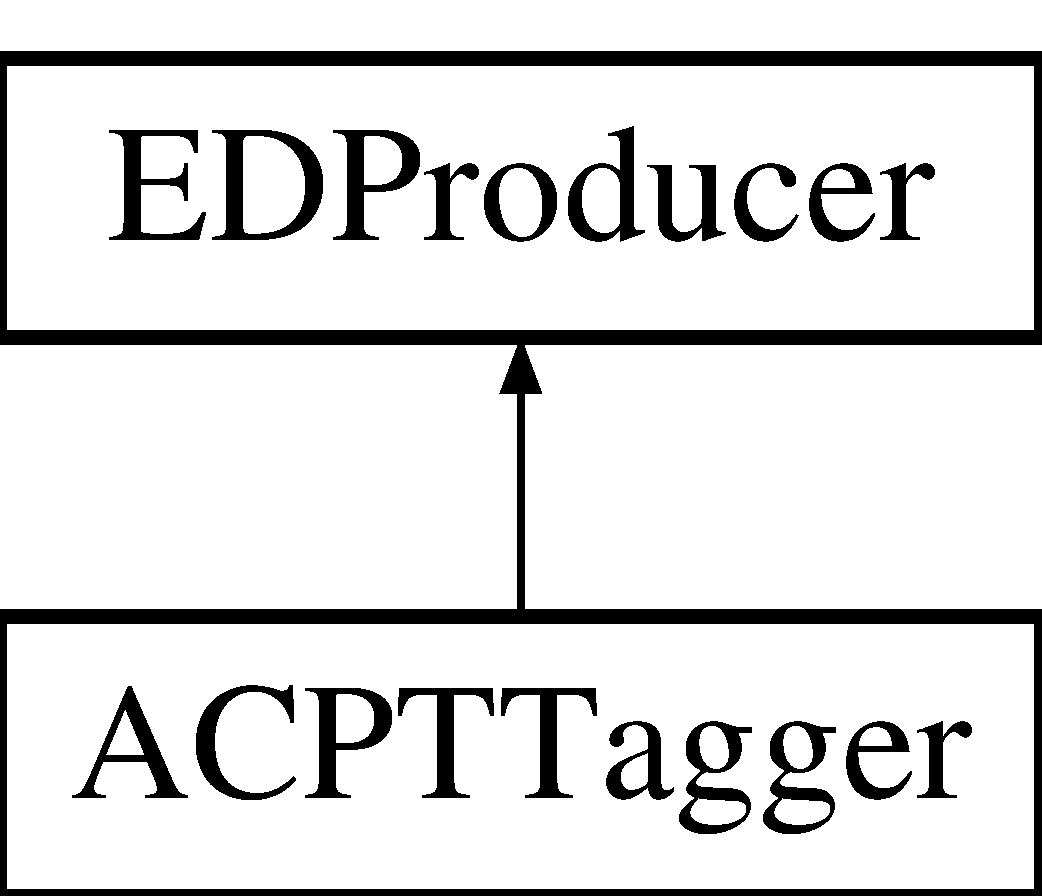
\includegraphics[height=2.000000cm]{classACPTTagger}
\end{center}
\end{figure}
\subsection*{Public Member Functions}
\begin{DoxyCompactItemize}
\item 
\hypertarget{classACPTTagger_a40826f58d28a7a25c0eeab2db30fa348}{{\bfseries A\-C\-P\-T\-Tagger} (fhicl\-::\-Parameter\-Set const \&p)}\label{classACPTTagger_a40826f58d28a7a25c0eeab2db30fa348}

\item 
\hypertarget{classACPTTagger_a97c00ff11dd51943192529d7532344f3}{{\bfseries A\-C\-P\-T\-Tagger} (\hyperlink{classACPTTagger}{A\-C\-P\-T\-Tagger} const \&)=delete}\label{classACPTTagger_a97c00ff11dd51943192529d7532344f3}

\item 
\hypertarget{classACPTTagger_acedfdf5c74d9ac721b5eb04420763c4f}{{\bfseries A\-C\-P\-T\-Tagger} (\hyperlink{classACPTTagger}{A\-C\-P\-T\-Tagger} \&\&)=delete}\label{classACPTTagger_acedfdf5c74d9ac721b5eb04420763c4f}

\item 
\hypertarget{classACPTTagger_afd87968bb97f886f421f588053423c63}{\hyperlink{classACPTTagger}{A\-C\-P\-T\-Tagger} \& {\bfseries operator=} (\hyperlink{classACPTTagger}{A\-C\-P\-T\-Tagger} const \&)=delete}\label{classACPTTagger_afd87968bb97f886f421f588053423c63}

\item 
\hypertarget{classACPTTagger_a4214057b2ad88e7e92393c5c005be228}{\hyperlink{classACPTTagger}{A\-C\-P\-T\-Tagger} \& {\bfseries operator=} (\hyperlink{classACPTTagger}{A\-C\-P\-T\-Tagger} \&\&)=delete}\label{classACPTTagger_a4214057b2ad88e7e92393c5c005be228}

\item 
\hypertarget{classACPTTagger_a263217e3f0e822270756d498623788fb}{void {\bfseries produce} (art\-::\-Event \&e) override}\label{classACPTTagger_a263217e3f0e822270756d498623788fb}

\end{DoxyCompactItemize}


The documentation for this class was generated from the following file\-:\begin{DoxyCompactItemize}
\item 
/home/travis/build/marcodeltutto/\-U\-B\-X\-Sec/\-Modules/A\-C\-P\-T\-Tagger\-\_\-module.\-cc\end{DoxyCompactItemize}

\hypertarget{structBoundaryWire}{\section{Boundary\-Wire Struct Reference}
\label{structBoundaryWire}\index{Boundary\-Wire@{Boundary\-Wire}}
}
\subsection*{Public Attributes}
\begin{DoxyCompactItemize}
\item 
\hypertarget{structBoundaryWire_aea1c09c6f1af43423698dd4d9ca0b86f}{unsigned int {\bfseries wire\-\_\-num}}\label{structBoundaryWire_aea1c09c6f1af43423698dd4d9ca0b86f}

\item 
\hypertarget{structBoundaryWire_a6969e3a2ea00f7a7f10e7a2a6add17a0}{float {\bfseries y\-\_\-start}}\label{structBoundaryWire_a6969e3a2ea00f7a7f10e7a2a6add17a0}

\item 
\hypertarget{structBoundaryWire_ac18920460b74370ddfaca7aaf2089283}{float {\bfseries z\-\_\-start}}\label{structBoundaryWire_ac18920460b74370ddfaca7aaf2089283}

\item 
\hypertarget{structBoundaryWire_a280aaa480170ff5f75b551e00993dc41}{float {\bfseries y\-\_\-end}}\label{structBoundaryWire_a280aaa480170ff5f75b551e00993dc41}

\item 
\hypertarget{structBoundaryWire_a5b3e58ad04ba75fb7c77cdb50cea3686}{float {\bfseries z\-\_\-end}}\label{structBoundaryWire_a5b3e58ad04ba75fb7c77cdb50cea3686}

\item 
\hypertarget{structBoundaryWire_a8ad92872ad08d86d9047a96d36255090}{bool {\bfseries is\-Low\-Wire}}\label{structBoundaryWire_a8ad92872ad08d86d9047a96d36255090}

\end{DoxyCompactItemize}


The documentation for this struct was generated from the following file\-:\begin{DoxyCompactItemize}
\item 
/home/travis/build/marcodeltutto/\-U\-B\-X\-Sec/\-Algorithms/\hyperlink{FindDeadRegions_8h}{Find\-Dead\-Regions.\-h}\end{DoxyCompactItemize}

\hypertarget{classCosmicFlashMatch}{\section{Cosmic\-Flash\-Match Class Reference}
\label{classCosmicFlashMatch}\index{Cosmic\-Flash\-Match@{Cosmic\-Flash\-Match}}
}
Inheritance diagram for Cosmic\-Flash\-Match\-:\begin{figure}[H]
\begin{center}
\leavevmode
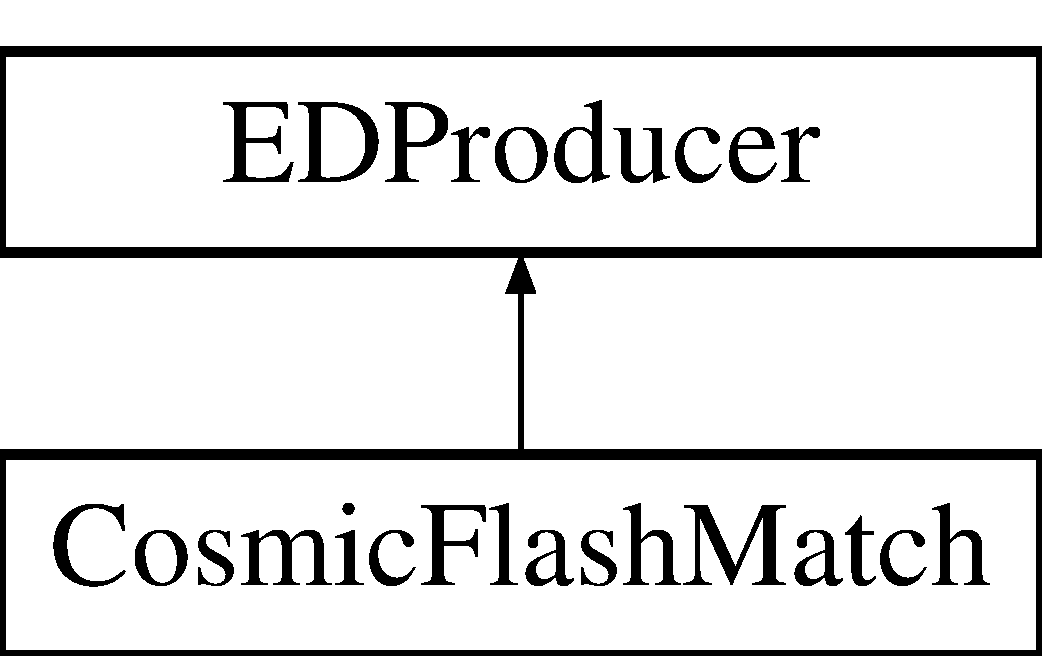
\includegraphics[height=2.000000cm]{classCosmicFlashMatch}
\end{center}
\end{figure}
\subsection*{Public Member Functions}
\begin{DoxyCompactItemize}
\item 
\hypertarget{classCosmicFlashMatch_a1b3ff330c64a20c3dd3e22c35f130cc4}{{\bfseries Cosmic\-Flash\-Match} (fhicl\-::\-Parameter\-Set const \&p)}\label{classCosmicFlashMatch_a1b3ff330c64a20c3dd3e22c35f130cc4}

\item 
\hypertarget{classCosmicFlashMatch_ad422dc1c69902d22d950786d02fcc2fa}{{\bfseries Cosmic\-Flash\-Match} (\hyperlink{classCosmicFlashMatch}{Cosmic\-Flash\-Match} const \&)=delete}\label{classCosmicFlashMatch_ad422dc1c69902d22d950786d02fcc2fa}

\item 
\hypertarget{classCosmicFlashMatch_a30c798d9283fea4385cc6ee0ae934a5c}{{\bfseries Cosmic\-Flash\-Match} (\hyperlink{classCosmicFlashMatch}{Cosmic\-Flash\-Match} \&\&)=delete}\label{classCosmicFlashMatch_a30c798d9283fea4385cc6ee0ae934a5c}

\item 
\hypertarget{classCosmicFlashMatch_a259c740b9a09a2cef24fba0b883fb873}{\hyperlink{classCosmicFlashMatch}{Cosmic\-Flash\-Match} \& {\bfseries operator=} (\hyperlink{classCosmicFlashMatch}{Cosmic\-Flash\-Match} const \&)=delete}\label{classCosmicFlashMatch_a259c740b9a09a2cef24fba0b883fb873}

\item 
\hypertarget{classCosmicFlashMatch_ada80618ce3d9ac661515e0af6369cd81}{\hyperlink{classCosmicFlashMatch}{Cosmic\-Flash\-Match} \& {\bfseries operator=} (\hyperlink{classCosmicFlashMatch}{Cosmic\-Flash\-Match} \&\&)=delete}\label{classCosmicFlashMatch_ada80618ce3d9ac661515e0af6369cd81}

\item 
\hypertarget{classCosmicFlashMatch_a8368e7181e2336eb079cb678113b3911}{void {\bfseries Get\-T\-P\-C\-Objects} (lar\-\_\-pandora\-::\-P\-F\-Particle\-Vector, lar\-\_\-pandora\-::\-P\-F\-Particles\-To\-Tracks, lar\-\_\-pandora\-::\-P\-F\-Particles\-To\-Vertices, std\-::vector$<$ lar\-\_\-pandora\-::\-P\-F\-Particle\-Vector $>$ \&, std\-::vector$<$ lar\-\_\-pandora\-::\-Track\-Vector $>$ \&)}\label{classCosmicFlashMatch_a8368e7181e2336eb079cb678113b3911}

\item 
\hypertarget{classCosmicFlashMatch_a04fb198244e86fbd2cb6c6f6a0ef1363}{flashana\-::\-Q\-Cluster\-\_\-t {\bfseries Get\-Q\-Cluster} (std\-::vector$<$ art\-::\-Ptr$<$ recob\-::\-Track $>$$>$)}\label{classCosmicFlashMatch_a04fb198244e86fbd2cb6c6f6a0ef1363}

\item 
\hypertarget{classCosmicFlashMatch_a29112dc33d6ce0be700ad02f967d709d}{void {\bfseries Collect\-Tracks\-And\-P\-F\-P} (lar\-\_\-pandora\-::\-P\-F\-Particles\-To\-Tracks, lar\-\_\-pandora\-::\-P\-F\-Particle\-Vector, art\-::\-Ptr$<$ recob\-::\-P\-F\-Particle $>$, lar\-\_\-pandora\-::\-P\-F\-Particle\-Vector \&, lar\-\_\-pandora\-::\-Track\-Vector \&)}\label{classCosmicFlashMatch_a29112dc33d6ce0be700ad02f967d709d}

\item 
\hypertarget{classCosmicFlashMatch_a3208db108dea02a5c7113205137ea363}{int {\bfseries Get\-Trajectory} (std\-::vector$<$ art\-::\-Ptr$<$ recob\-::\-Track $>$$>$,\-::geoalgo\-::\-Trajectory \&)}\label{classCosmicFlashMatch_a3208db108dea02a5c7113205137ea363}

\item 
\hypertarget{classCosmicFlashMatch_ac329a3c7f942e9c7d26ecee88f91c8ea}{flashana\-::\-Flash\-\_\-t {\bfseries Trial} (std\-::vector$<$ art\-::\-Ptr$<$ recob\-::\-Track $>$$>$ track\-\_\-v, flashana\-::\-Flash\-\_\-t flash\-Beam, double \&\-\_\-chi2, double \&\-\_\-ll)}\label{classCosmicFlashMatch_ac329a3c7f942e9c7d26ecee88f91c8ea}

\item 
\hypertarget{classCosmicFlashMatch_aebcbe54d9d6fc9e14b98a008d7776308}{void {\bfseries produce} (art\-::\-Event \&e) override}\label{classCosmicFlashMatch_aebcbe54d9d6fc9e14b98a008d7776308}

\end{DoxyCompactItemize}


The documentation for this class was generated from the following file\-:\begin{DoxyCompactItemize}
\item 
/home/travis/build/marcodeltutto/\-U\-B\-X\-Sec/\-Modules/Cosmic\-Flash\-Match\-\_\-module.\-cc\end{DoxyCompactItemize}

\hypertarget{classCosmicTagByHitIntegral}{\section{Cosmic\-Tag\-By\-Hit\-Integral Class Reference}
\label{classCosmicTagByHitIntegral}\index{Cosmic\-Tag\-By\-Hit\-Integral@{Cosmic\-Tag\-By\-Hit\-Integral}}
}


Cosmic\-Tag.  




{\ttfamily \#include $<$Cosmic\-Tag\-By\-Hit\-Integral.\-h$>$}



\subsection{Detailed Description}
Cosmic\-Tag. 

\begin{DoxyAuthor}{Author}

\end{DoxyAuthor}
\begin{DoxyParagraph}{Author\-:}
Marco Del Tutto\href{mailto:marco.deltutto@physics.ox.ac.uk}{\tt marco.\-deltutto@physics.\-ox.\-ac.\-uk} 
\end{DoxyParagraph}


\begin{DoxyVersion}{Version}

\end{DoxyVersion}
\begin{DoxyParagraph}{Revision\-:}
1.\-0 
\end{DoxyParagraph}


\begin{DoxyDate}{Date}

\end{DoxyDate}
\begin{DoxyParagraph}{Date\-:}
2017/08/18 
\end{DoxyParagraph}


Contact\-: \href{mailto:marco.deltutto@physics.ox.ac.uk}{\tt marco.\-deltutto@physics.\-ox.\-ac.\-uk}

Created on\-: Friday, August 18, 2017 at 08\-:53\-:50 

The documentation for this class was generated from the following file\-:\begin{DoxyCompactItemize}
\item 
/home/travis/build/marcodeltutto/\-U\-B\-X\-Sec/\-Algorithms/Cosmic\-Tag\-By\-Hit\-Integral.\-h\end{DoxyCompactItemize}

\hypertarget{classubana_1_1CosmicTagByHitIntegral}{\section{ubana\-:\-:Cosmic\-Tag\-By\-Hit\-Integral Class Reference}
\label{classubana_1_1CosmicTagByHitIntegral}\index{ubana\-::\-Cosmic\-Tag\-By\-Hit\-Integral@{ubana\-::\-Cosmic\-Tag\-By\-Hit\-Integral}}
}
Inheritance diagram for ubana\-:\-:Cosmic\-Tag\-By\-Hit\-Integral\-:\begin{figure}[H]
\begin{center}
\leavevmode
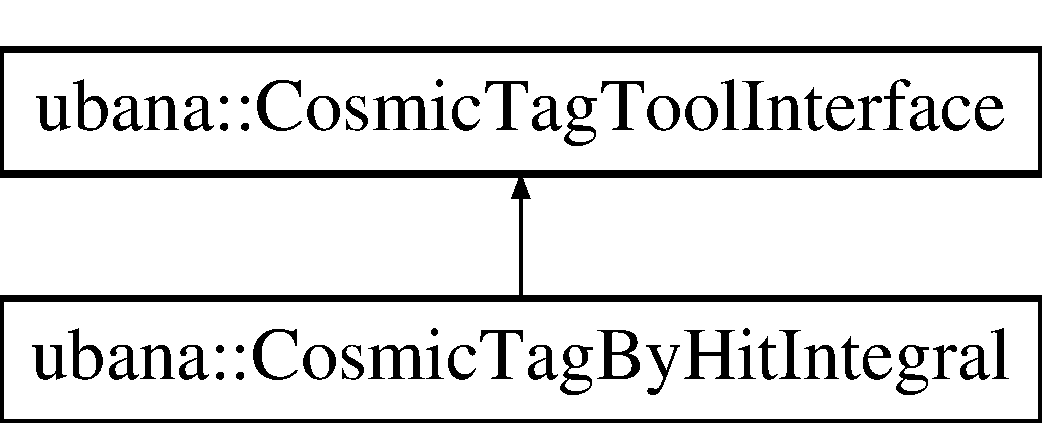
\includegraphics[height=2.000000cm]{classubana_1_1CosmicTagByHitIntegral}
\end{center}
\end{figure}
\subsection*{Public Member Functions}
\begin{DoxyCompactItemize}
\item 
\hypertarget{classubana_1_1CosmicTagByHitIntegral_ae58970463cfcb6fa697e19073da6a91c}{\hyperlink{classubana_1_1CosmicTagByHitIntegral_ae58970463cfcb6fa697e19073da6a91c}{Cosmic\-Tag\-By\-Hit\-Integral} (fhicl\-::\-Parameter\-Set const \&ps)}\label{classubana_1_1CosmicTagByHitIntegral_ae58970463cfcb6fa697e19073da6a91c}

\begin{DoxyCompactList}\small\item\em Constructor. \end{DoxyCompactList}\item 
\hypertarget{classubana_1_1CosmicTagByHitIntegral_ad51d5460821d3a81262f8515a8e08487}{\hyperlink{classubana_1_1CosmicTagByHitIntegral_ad51d5460821d3a81262f8515a8e08487}{Cosmic\-Tag\-By\-Hit\-Integral} ()}\label{classubana_1_1CosmicTagByHitIntegral_ad51d5460821d3a81262f8515a8e08487}

\begin{DoxyCompactList}\small\item\em Constructor. \end{DoxyCompactList}\item 
\hypertarget{classubana_1_1CosmicTagByHitIntegral_a33a59b4d8c00231b368879a591e80b5c}{bool \hyperlink{classubana_1_1CosmicTagByHitIntegral_a33a59b4d8c00231b368879a591e80b5c}{Is\-Cosmic} (Simple\-Hit\-Vector) override}\label{classubana_1_1CosmicTagByHitIntegral_a33a59b4d8c00231b368879a591e80b5c}

\begin{DoxyCompactList}\small\item\em Description. \end{DoxyCompactList}\end{DoxyCompactItemize}


The documentation for this class was generated from the following files\-:\begin{DoxyCompactItemize}
\item 
/home/travis/build/marcodeltutto/\-U\-B\-X\-Sec/\-Algorithms/Cosmic\-Tag\-By\-Hit\-Integral.\-h\item 
/home/travis/build/marcodeltutto/\-U\-B\-X\-Sec/\-Algorithms/Cosmic\-Tag\-By\-Hit\-Integral.\-cxx\end{DoxyCompactItemize}

\hypertarget{classCosmicTaggerAna}{\section{Cosmic\-Tagger\-Ana Class Reference}
\label{classCosmicTaggerAna}\index{Cosmic\-Tagger\-Ana@{Cosmic\-Tagger\-Ana}}
}
Inheritance diagram for Cosmic\-Tagger\-Ana\-:\begin{figure}[H]
\begin{center}
\leavevmode
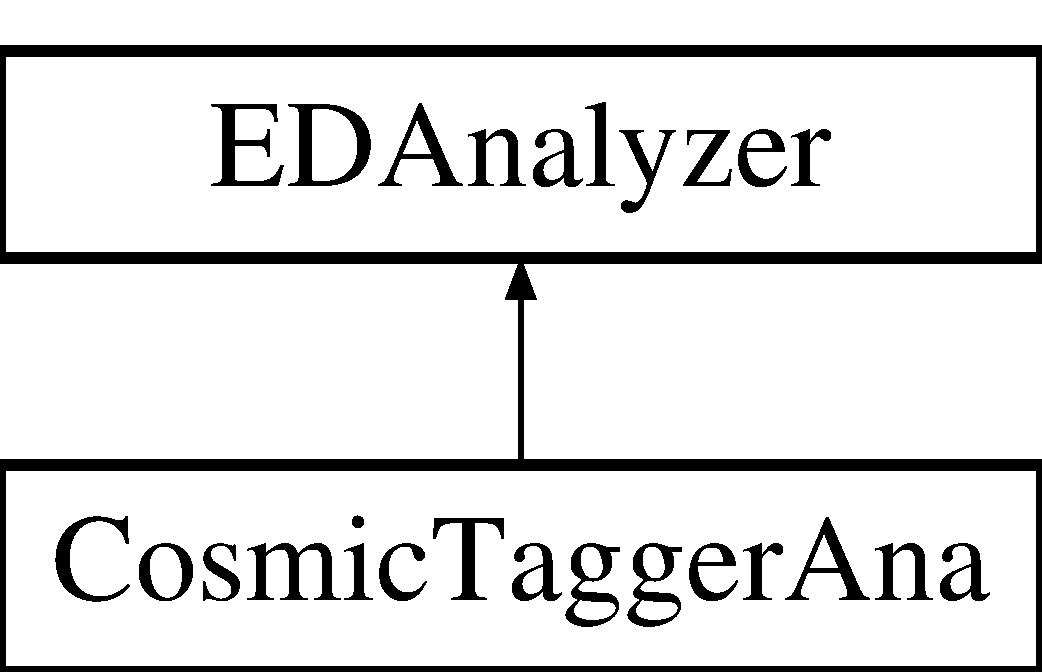
\includegraphics[height=2.000000cm]{classCosmicTaggerAna}
\end{center}
\end{figure}
\subsection*{Public Member Functions}
\begin{DoxyCompactItemize}
\item 
\hypertarget{classCosmicTaggerAna_a057039c409136601ac09420faf77c099}{{\bfseries Cosmic\-Tagger\-Ana} (fhicl\-::\-Parameter\-Set const \&p)}\label{classCosmicTaggerAna_a057039c409136601ac09420faf77c099}

\item 
\hypertarget{classCosmicTaggerAna_ae97386c9238c955b1b84fabe9ad2803c}{{\bfseries Cosmic\-Tagger\-Ana} (\hyperlink{classCosmicTaggerAna}{Cosmic\-Tagger\-Ana} const \&)=delete}\label{classCosmicTaggerAna_ae97386c9238c955b1b84fabe9ad2803c}

\item 
\hypertarget{classCosmicTaggerAna_aaa8d188e33c5787293c92dfcb99679c3}{{\bfseries Cosmic\-Tagger\-Ana} (\hyperlink{classCosmicTaggerAna}{Cosmic\-Tagger\-Ana} \&\&)=delete}\label{classCosmicTaggerAna_aaa8d188e33c5787293c92dfcb99679c3}

\item 
\hypertarget{classCosmicTaggerAna_ab28bec4bf2d71de7f6adcaa6d57a8c50}{\hyperlink{classCosmicTaggerAna}{Cosmic\-Tagger\-Ana} \& {\bfseries operator=} (\hyperlink{classCosmicTaggerAna}{Cosmic\-Tagger\-Ana} const \&)=delete}\label{classCosmicTaggerAna_ab28bec4bf2d71de7f6adcaa6d57a8c50}

\item 
\hypertarget{classCosmicTaggerAna_a0ff825d46a57593ef95d8139b92861a8}{\hyperlink{classCosmicTaggerAna}{Cosmic\-Tagger\-Ana} \& {\bfseries operator=} (\hyperlink{classCosmicTaggerAna}{Cosmic\-Tagger\-Ana} \&\&)=delete}\label{classCosmicTaggerAna_a0ff825d46a57593ef95d8139b92861a8}

\item 
\hypertarget{classCosmicTaggerAna_aea04b9a8752a0730aa18c81d298decf9}{void {\bfseries analyze} (art\-::\-Event const \&e) override}\label{classCosmicTaggerAna_aea04b9a8752a0730aa18c81d298decf9}

\end{DoxyCompactItemize}


The documentation for this class was generated from the following file\-:\begin{DoxyCompactItemize}
\item 
/home/travis/build/marcodeltutto/\-U\-B\-X\-Sec/\-Modules/Cosmic\-Tagger\-Ana\-\_\-module.\-cc\end{DoxyCompactItemize}

\hypertarget{classCosmicTagToolInterface}{\section{\-Cosmic\-Tag\-Tool\-Interface \-Class \-Reference}
\label{classCosmicTagToolInterface}\index{\-Cosmic\-Tag\-Tool\-Interface@{\-Cosmic\-Tag\-Tool\-Interface}}
}


\-Interface for art module.  




{\ttfamily \#include $<$\-Cosmic\-Tag\-Tool\-Interface.\-h$>$}



\subsection{\-Detailed \-Description}
\-Interface for art module. 

\begin{DoxyAuthor}{\-Author}

\end{DoxyAuthor}
\begin{DoxyParagraph}{\-Author\-:}
\-Marco \-Del \-Tutto$<$\href{mailto:marco.deltutto@physics.ox.ac.uk}{\tt marco.\-deltutto@physics.\-ox.\-ac.\-uk}$>$ 
\end{DoxyParagraph}


\begin{DoxyVersion}{\-Version}

\end{DoxyVersion}
\begin{DoxyParagraph}{\-Revision\-:}
1.\-0 
\end{DoxyParagraph}


\begin{DoxyDate}{\-Date}

\end{DoxyDate}
\begin{DoxyParagraph}{\-Date\-:}
2017/08/18 
\end{DoxyParagraph}


\-Contact\-: \href{mailto:marco.deltutto@physics.ox.ac.uk}{\tt marco.\-deltutto@physics.\-ox.\-ac.\-uk}

\-Created on\-: \-Friday, \-August 18, 2017 at 08\-:53\-:50 

\-The documentation for this class was generated from the following file\-:\begin{DoxyCompactItemize}
\item 
/home/travis/build/marcodeltutto/\-U\-B\-X\-Sec/\-Algorithms/\-Cosmic\-Tag\-Tool\-Interface.\-h\end{DoxyCompactItemize}

\hypertarget{classubana_1_1CosmicTagToolInterface}{\section{ubana\-:\-:\-Cosmic\-Tag\-Tool\-Interface \-Class \-Reference}
\label{classubana_1_1CosmicTagToolInterface}\index{ubana\-::\-Cosmic\-Tag\-Tool\-Interface@{ubana\-::\-Cosmic\-Tag\-Tool\-Interface}}
}
\-Inheritance diagram for ubana\-:\-:\-Cosmic\-Tag\-Tool\-Interface\-:\begin{figure}[H]
\begin{center}
\leavevmode
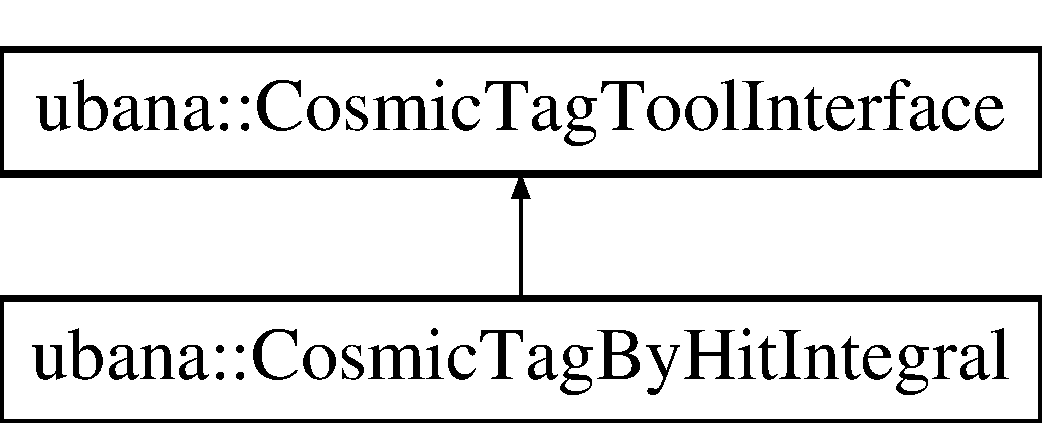
\includegraphics[height=2.000000cm]{classubana_1_1CosmicTagToolInterface}
\end{center}
\end{figure}
\subsection*{\-Public \-Member \-Functions}
\begin{DoxyCompactItemize}
\item 
\hypertarget{classubana_1_1CosmicTagToolInterface_a2c14c0575c5234efc433517b91b67683}{virtual \hyperlink{classubana_1_1CosmicTagToolInterface_a2c14c0575c5234efc433517b91b67683}{$\sim$\-Cosmic\-Tag\-Tool\-Interface} () noexcept}\label{classubana_1_1CosmicTagToolInterface_a2c14c0575c5234efc433517b91b67683}

\begin{DoxyCompactList}\small\item\em \-Default destructor. \end{DoxyCompactList}\item 
\hypertarget{classubana_1_1CosmicTagToolInterface_a5363b61b1dfab1e6b9cade4b3eed2c66}{virtual bool \hyperlink{classubana_1_1CosmicTagToolInterface_a5363b61b1dfab1e6b9cade4b3eed2c66}{\-Is\-Cosmic} (\-Simple\-Hit\-Vector)=0}\label{classubana_1_1CosmicTagToolInterface_a5363b61b1dfab1e6b9cade4b3eed2c66}

\begin{DoxyCompactList}\small\item\em \-Performs the matching. \end{DoxyCompactList}\end{DoxyCompactItemize}


\-The documentation for this class was generated from the following file\-:\begin{DoxyCompactItemize}
\item 
/home/travis/build/marcodeltutto/\-U\-B\-X\-Sec/\-Algorithms/\-Cosmic\-Tag\-Tool\-Interface.\-h\end{DoxyCompactItemize}

\hypertarget{classCosmicTrackHitTagger}{\section{Cosmic\-Track\-Hit\-Tagger Class Reference}
\label{classCosmicTrackHitTagger}\index{Cosmic\-Track\-Hit\-Tagger@{Cosmic\-Track\-Hit\-Tagger}}
}
Inheritance diagram for Cosmic\-Track\-Hit\-Tagger\-:\begin{figure}[H]
\begin{center}
\leavevmode
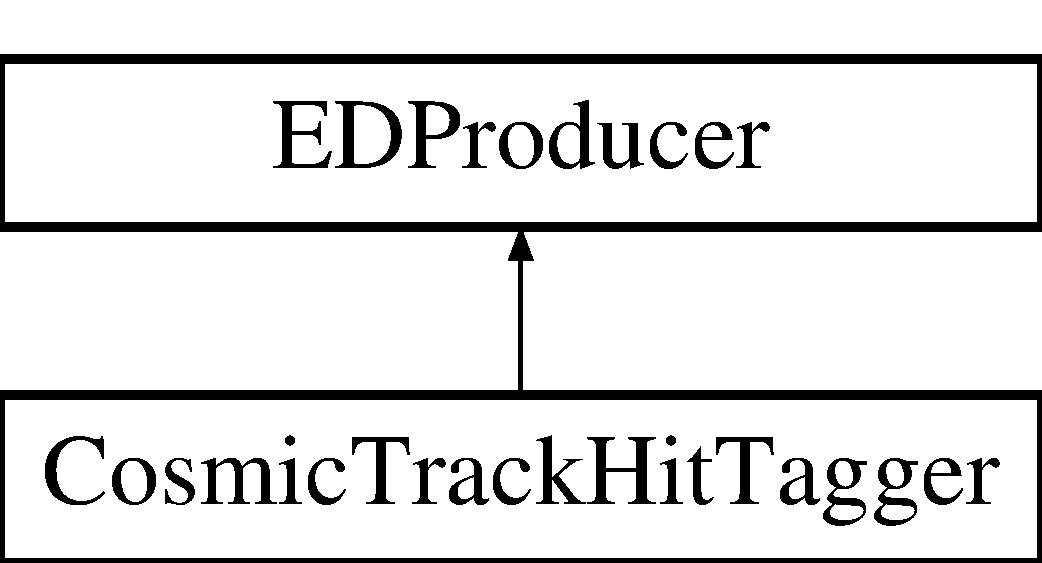
\includegraphics[height=2.000000cm]{classCosmicTrackHitTagger}
\end{center}
\end{figure}
\subsection*{Public Member Functions}
\begin{DoxyCompactItemize}
\item 
\hypertarget{classCosmicTrackHitTagger_ac6a0456ac0a13fd69a9ff4b02882f0a5}{{\bfseries Cosmic\-Track\-Hit\-Tagger} (fhicl\-::\-Parameter\-Set const \&p)}\label{classCosmicTrackHitTagger_ac6a0456ac0a13fd69a9ff4b02882f0a5}

\item 
\hypertarget{classCosmicTrackHitTagger_a13c4dc2408621b6f4de50f08254025c8}{{\bfseries Cosmic\-Track\-Hit\-Tagger} (\hyperlink{classCosmicTrackHitTagger}{Cosmic\-Track\-Hit\-Tagger} const \&)=delete}\label{classCosmicTrackHitTagger_a13c4dc2408621b6f4de50f08254025c8}

\item 
\hypertarget{classCosmicTrackHitTagger_a319a011ab3346cea74fc81df39cc9cc7}{{\bfseries Cosmic\-Track\-Hit\-Tagger} (\hyperlink{classCosmicTrackHitTagger}{Cosmic\-Track\-Hit\-Tagger} \&\&)=delete}\label{classCosmicTrackHitTagger_a319a011ab3346cea74fc81df39cc9cc7}

\item 
\hypertarget{classCosmicTrackHitTagger_aa68ec7260c542d56f781add788855053}{\hyperlink{classCosmicTrackHitTagger}{Cosmic\-Track\-Hit\-Tagger} \& {\bfseries operator=} (\hyperlink{classCosmicTrackHitTagger}{Cosmic\-Track\-Hit\-Tagger} const \&)=delete}\label{classCosmicTrackHitTagger_aa68ec7260c542d56f781add788855053}

\item 
\hypertarget{classCosmicTrackHitTagger_a2283b66a71b24975ef28369064440062}{\hyperlink{classCosmicTrackHitTagger}{Cosmic\-Track\-Hit\-Tagger} \& {\bfseries operator=} (\hyperlink{classCosmicTrackHitTagger}{Cosmic\-Track\-Hit\-Tagger} \&\&)=delete}\label{classCosmicTrackHitTagger_a2283b66a71b24975ef28369064440062}

\item 
\hypertarget{classCosmicTrackHitTagger_a6ffc6038717475e1887296c8b4fbacae}{void {\bfseries produce} (art\-::\-Event \&e) override}\label{classCosmicTrackHitTagger_a6ffc6038717475e1887296c8b4fbacae}

\end{DoxyCompactItemize}


The documentation for this class was generated from the following file\-:\begin{DoxyCompactItemize}
\item 
/home/travis/build/marcodeltutto/\-U\-B\-X\-Sec/\-Modules/Cosmic\-Track\-Hit\-Tagger\-\_\-module.\-cc\end{DoxyCompactItemize}

\hypertarget{classDeDxAna}{\section{De\-Dx\-Ana Class Reference}
\label{classDeDxAna}\index{De\-Dx\-Ana@{De\-Dx\-Ana}}
}
Inheritance diagram for De\-Dx\-Ana\-:\begin{figure}[H]
\begin{center}
\leavevmode
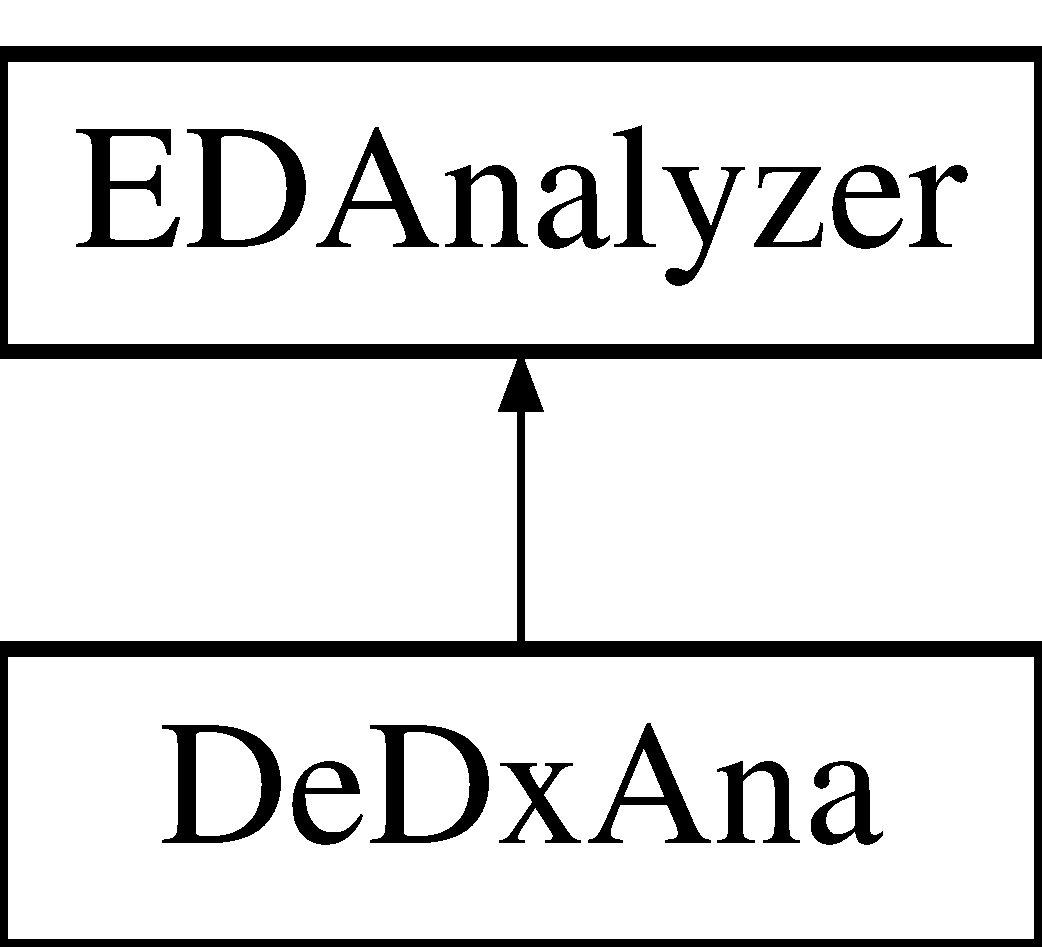
\includegraphics[height=2.000000cm]{classDeDxAna}
\end{center}
\end{figure}
\subsection*{Public Member Functions}
\begin{DoxyCompactItemize}
\item 
\hypertarget{classDeDxAna_aafa017bdd99fff476da1a0fc5ea67722}{{\bfseries De\-Dx\-Ana} (fhicl\-::\-Parameter\-Set const \&p)}\label{classDeDxAna_aafa017bdd99fff476da1a0fc5ea67722}

\item 
\hypertarget{classDeDxAna_a7a0e448252c3a8a85dbedd88b9acde41}{{\bfseries De\-Dx\-Ana} (\hyperlink{classDeDxAna}{De\-Dx\-Ana} const \&)=delete}\label{classDeDxAna_a7a0e448252c3a8a85dbedd88b9acde41}

\item 
\hypertarget{classDeDxAna_a9bd2425ac117a5502b146e79688042b6}{{\bfseries De\-Dx\-Ana} (\hyperlink{classDeDxAna}{De\-Dx\-Ana} \&\&)=delete}\label{classDeDxAna_a9bd2425ac117a5502b146e79688042b6}

\item 
\hypertarget{classDeDxAna_a2168024a40002cf6b3b4aa25df99faa4}{\hyperlink{classDeDxAna}{De\-Dx\-Ana} \& {\bfseries operator=} (\hyperlink{classDeDxAna}{De\-Dx\-Ana} const \&)=delete}\label{classDeDxAna_a2168024a40002cf6b3b4aa25df99faa4}

\item 
\hypertarget{classDeDxAna_a3b71a1570272d521eabef8d7468eac82}{\hyperlink{classDeDxAna}{De\-Dx\-Ana} \& {\bfseries operator=} (\hyperlink{classDeDxAna}{De\-Dx\-Ana} \&\&)=delete}\label{classDeDxAna_a3b71a1570272d521eabef8d7468eac82}

\item 
\hypertarget{classDeDxAna_a997e03e16044d2e5c8603cc6578c43c3}{void {\bfseries analyze} (art\-::\-Event const \&e) override}\label{classDeDxAna_a997e03e16044d2e5c8603cc6578c43c3}

\end{DoxyCompactItemize}


The documentation for this class was generated from the following file\-:\begin{DoxyCompactItemize}
\item 
/home/travis/build/marcodeltutto/\-U\-B\-X\-Sec/\-Modules/De\-Dx\-Ana\-\_\-module.\-cc\end{DoxyCompactItemize}

\hypertarget{classubana_1_1FiducialVolume}{\section{ubana\-:\-:Fiducial\-Volume Class Reference}
\label{classubana_1_1FiducialVolume}\index{ubana\-::\-Fiducial\-Volume@{ubana\-::\-Fiducial\-Volume}}
}


{\ttfamily \#include $<$Fiducial\-Volume.\-h$>$}

\subsection*{Public Member Functions}
\begin{DoxyCompactItemize}
\item 
\hypertarget{classubana_1_1FiducialVolume_a557d2e3c2d7b6151ea0156685bf56d00}{\hyperlink{classubana_1_1FiducialVolume_a557d2e3c2d7b6151ea0156685bf56d00}{Fiducial\-Volume} ()}\label{classubana_1_1FiducialVolume_a557d2e3c2d7b6151ea0156685bf56d00}

\begin{DoxyCompactList}\small\item\em Default constructor. \end{DoxyCompactList}\item 
\hypertarget{classubana_1_1FiducialVolume_adf150e608c658207370667f6130947a6}{\hyperlink{classubana_1_1FiducialVolume_adf150e608c658207370667f6130947a6}{$\sim$\-Fiducial\-Volume} ()}\label{classubana_1_1FiducialVolume_adf150e608c658207370667f6130947a6}

\begin{DoxyCompactList}\small\item\em Default destructor. \end{DoxyCompactList}\item 
\hypertarget{classubana_1_1FiducialVolume_a1a7d659cde6b1f4b661ca21df6677fd9}{void \hyperlink{classubana_1_1FiducialVolume_a1a7d659cde6b1f4b661ca21df6677fd9}{Configure} (fhicl\-::\-Parameter\-Set const \&p, double det\-\_\-half\-\_\-height, double det\-\_\-width, double det\-\_\-length)}\label{classubana_1_1FiducialVolume_a1a7d659cde6b1f4b661ca21df6677fd9}

\begin{DoxyCompactList}\small\item\em Configure function parameters. \end{DoxyCompactList}\item 
\hypertarget{classubana_1_1FiducialVolume_a852522fe049681771c7ca9d66f8f8049}{void \hyperlink{classubana_1_1FiducialVolume_a852522fe049681771c7ca9d66f8f8049}{Print\-Config} ()}\label{classubana_1_1FiducialVolume_a852522fe049681771c7ca9d66f8f8049}

\begin{DoxyCompactList}\small\item\em Printd the current configuration. \end{DoxyCompactList}\item 
\hypertarget{classubana_1_1FiducialVolume_a7c1752435937f91d70e262d7632b3227}{bool \hyperlink{classubana_1_1FiducialVolume_a7c1752435937f91d70e262d7632b3227}{In\-F\-V} (double x, double y, double z)}\label{classubana_1_1FiducialVolume_a7c1752435937f91d70e262d7632b3227}

\begin{DoxyCompactList}\small\item\em Returns true if the point is in the F\-V. \end{DoxyCompactList}\item 
\hypertarget{classubana_1_1FiducialVolume_aa41233ef6232819c491953b798c40ac9}{bool \hyperlink{classubana_1_1FiducialVolume_aa41233ef6232819c491953b798c40ac9}{In\-F\-V} (double $\ast$x)}\label{classubana_1_1FiducialVolume_aa41233ef6232819c491953b798c40ac9}

\begin{DoxyCompactList}\small\item\em Returns true if the point is in the F\-V. \end{DoxyCompactList}\item 
\hypertarget{classubana_1_1FiducialVolume_a9e0d67156adcdec097f8b8286fac8105}{bool \hyperlink{classubana_1_1FiducialVolume_a9e0d67156adcdec097f8b8286fac8105}{In\-F\-V} (T\-Vector3 x)}\label{classubana_1_1FiducialVolume_a9e0d67156adcdec097f8b8286fac8105}

\begin{DoxyCompactList}\small\item\em Returns true if the point is in the F\-V. \end{DoxyCompactList}\item 
\hypertarget{classubana_1_1FiducialVolume_ad930931de1d711775762e490e5b07a1a}{bool \hyperlink{classubana_1_1FiducialVolume_ad930931de1d711775762e490e5b07a1a}{In\-F\-V} (T\-Vector3 x1, T\-Vector3 x2)}\label{classubana_1_1FiducialVolume_ad930931de1d711775762e490e5b07a1a}

\begin{DoxyCompactList}\small\item\em Returns true if B\-O\-T\-H points are in the F\-V. \end{DoxyCompactList}\end{DoxyCompactItemize}
\subsection*{Protected Attributes}
\begin{DoxyCompactItemize}
\item 
\hypertarget{classubana_1_1FiducialVolume_aa96f6087fbf3df5fefb0a38bf2821ca7}{double {\bfseries \-\_\-det\-\_\-half\-\_\-height}}\label{classubana_1_1FiducialVolume_aa96f6087fbf3df5fefb0a38bf2821ca7}

\item 
\hypertarget{classubana_1_1FiducialVolume_aa6d8cc1ba873cf5ada02b3072168d4c2}{double {\bfseries \-\_\-det\-\_\-width}}\label{classubana_1_1FiducialVolume_aa6d8cc1ba873cf5ada02b3072168d4c2}

\item 
\hypertarget{classubana_1_1FiducialVolume_aeab2a2472cc090816d5dcfdef27c1059}{double {\bfseries \-\_\-det\-\_\-length}}\label{classubana_1_1FiducialVolume_aeab2a2472cc090816d5dcfdef27c1059}

\item 
\hypertarget{classubana_1_1FiducialVolume_ade7d6cc1ab834c474aa01f9940b201c5}{double {\bfseries \-\_\-border\-\_\-x\-\_\-low}}\label{classubana_1_1FiducialVolume_ade7d6cc1ab834c474aa01f9940b201c5}

\item 
\hypertarget{classubana_1_1FiducialVolume_a212325c987333920fbcd9ccc62719066}{double {\bfseries \-\_\-border\-\_\-x\-\_\-high}}\label{classubana_1_1FiducialVolume_a212325c987333920fbcd9ccc62719066}

\item 
\hypertarget{classubana_1_1FiducialVolume_a23422b2d254a3434c580f4a39d4b6ba1}{double {\bfseries \-\_\-border\-\_\-y\-\_\-low}}\label{classubana_1_1FiducialVolume_a23422b2d254a3434c580f4a39d4b6ba1}

\item 
\hypertarget{classubana_1_1FiducialVolume_a361f7b780053a650de50d64c65d99d45}{double {\bfseries \-\_\-border\-\_\-y\-\_\-high}}\label{classubana_1_1FiducialVolume_a361f7b780053a650de50d64c65d99d45}

\item 
\hypertarget{classubana_1_1FiducialVolume_ab941e99a432dc6fc5f5621db6c40cdbd}{double {\bfseries \-\_\-border\-\_\-z\-\_\-low}}\label{classubana_1_1FiducialVolume_ab941e99a432dc6fc5f5621db6c40cdbd}

\item 
\hypertarget{classubana_1_1FiducialVolume_a99d52085f4175cc3e5b99eb1418b1473}{double {\bfseries \-\_\-border\-\_\-z\-\_\-high}}\label{classubana_1_1FiducialVolume_a99d52085f4175cc3e5b99eb1418b1473}

\item 
\hypertarget{classubana_1_1FiducialVolume_a69587a1be20d319f9b9549ee36908890}{bool {\bfseries \-\_\-configured} = false}\label{classubana_1_1FiducialVolume_a69587a1be20d319f9b9549ee36908890}

\end{DoxyCompactItemize}


\subsection{Detailed Description}
User defined class \hyperlink{classubana_1_1FiducialVolume}{Fiducial\-Volume} ... these comments are used to generate doxygen documentation! 

The documentation for this class was generated from the following files\-:\begin{DoxyCompactItemize}
\item 
/home/travis/build/marcodeltutto/\-U\-B\-X\-Sec/\-Algorithms/\hyperlink{FiducialVolume_8h}{Fiducial\-Volume.\-h}\item 
/home/travis/build/marcodeltutto/\-U\-B\-X\-Sec/\-Algorithms/Fiducial\-Volume.\-cxx\end{DoxyCompactItemize}

\hypertarget{classFindDeadRegions}{\section{Find\-Dead\-Regions Class Reference}
\label{classFindDeadRegions}\index{Find\-Dead\-Regions@{Find\-Dead\-Regions}}
}
\subsection*{Public Member Functions}
\begin{DoxyCompactItemize}
\item 
\hypertarget{classFindDeadRegions_a94b207b673c58df861537ead4ec5385a}{void \hyperlink{classFindDeadRegions_a94b207b673c58df861537ead4ec5385a}{Configure} (fhicl\-::\-Parameter\-Set const \&p)}\label{classFindDeadRegions_a94b207b673c58df861537ead4ec5385a}

\begin{DoxyCompactList}\small\item\em Configure function parameters. \end{DoxyCompactList}\item 
\hypertarget{classFindDeadRegions_a7a884dc4685e66734b98afea9a2c6c21}{bool \hyperlink{classFindDeadRegions_a7a884dc4685e66734b98afea9a2c6c21}{Near\-Dead\-Reg2\-P} (float y\-Val, float z\-Val, float tolerance)}\label{classFindDeadRegions_a7a884dc4685e66734b98afea9a2c6c21}

\begin{DoxyCompactList}\small\item\em Returns true if the passed point is close to a dead region given a tolerance considering two planes only. \end{DoxyCompactList}\item 
\hypertarget{classFindDeadRegions_a2ef76eca81785361bf95c17e8e1a7574}{bool \hyperlink{classFindDeadRegions_a2ef76eca81785361bf95c17e8e1a7574}{Near\-Dead\-Reg3\-P} (float y\-Val, float z\-Val, float tolerance)}\label{classFindDeadRegions_a2ef76eca81785361bf95c17e8e1a7574}

\begin{DoxyCompactList}\small\item\em Returns true if the passed point is close to a dead region given a tolerance considering all three planes. \end{DoxyCompactList}\item 
\hypertarget{classFindDeadRegions_a712767abce6132b0dd6638a335da87fa}{T\-H2\-F $\ast$ \hyperlink{classFindDeadRegions_a712767abce6132b0dd6638a335da87fa}{Get\-Dead\-Region\-Histo2\-P} ()}\label{classFindDeadRegions_a712767abce6132b0dd6638a335da87fa}

\begin{DoxyCompactList}\small\item\em Returns a root 2\-D histogram (y v.\-s. z) containing the detector dead regions considering two planes only. \end{DoxyCompactList}\item 
\hypertarget{classFindDeadRegions_a93fcf74bb534831495f50a79fede19f9}{void \hyperlink{classFindDeadRegions_a93fcf74bb534831495f50a79fede19f9}{Get\-Dead\-Region\-Histo2\-P} (T\-H2\-F $\ast$)}\label{classFindDeadRegions_a93fcf74bb534831495f50a79fede19f9}

\begin{DoxyCompactList}\small\item\em Returns a root 2\-D histogram (y v.\-s. z) containing the detector dead regions considering two planes only. \end{DoxyCompactList}\item 
\hypertarget{classFindDeadRegions_abb378991861e7fdef4cd94a27d52ec07}{T\-H2\-F $\ast$ \hyperlink{classFindDeadRegions_abb378991861e7fdef4cd94a27d52ec07}{Get\-Dead\-Region\-Histo3\-P} ()}\label{classFindDeadRegions_abb378991861e7fdef4cd94a27d52ec07}

\begin{DoxyCompactList}\small\item\em Returns a root 2\-D histogram (y v.\-s. z) containing the detector dead regions considering all three planes. \end{DoxyCompactList}\item 
\hypertarget{classFindDeadRegions_a50de57c6d1792a6f2a93df8a44ba840a}{void \hyperlink{classFindDeadRegions_a50de57c6d1792a6f2a93df8a44ba840a}{Get\-Dead\-Region\-Histo3\-P} (T\-H2\-F $\ast$)}\label{classFindDeadRegions_a50de57c6d1792a6f2a93df8a44ba840a}

\begin{DoxyCompactList}\small\item\em Returns a root 2\-D histogram (y v.\-s. z) containing the detector dead regions considering all three planes. \end{DoxyCompactList}\end{DoxyCompactItemize}


The documentation for this class was generated from the following files\-:\begin{DoxyCompactItemize}
\item 
/home/travis/build/marcodeltutto/\-U\-B\-X\-Sec/\-Algorithms/\hyperlink{FindDeadRegions_8h}{Find\-Dead\-Regions.\-h}\item 
/home/travis/build/marcodeltutto/\-U\-B\-X\-Sec/\-Algorithms/Find\-Dead\-Regions.\-cxx\end{DoxyCompactItemize}

\hypertarget{classubana_1_1FlashMatch}{\section{ubana\-:\-:Flash\-Match Class Reference}
\label{classubana_1_1FlashMatch}\index{ubana\-::\-Flash\-Match@{ubana\-::\-Flash\-Match}}
}


Data product to store a flash matching results.  




{\ttfamily \#include $<$Flash\-Match.\-h$>$}

\subsection*{Public Member Functions}
\begin{DoxyCompactItemize}
\item 
\hypertarget{classubana_1_1FlashMatch_ac6dac027acf7a820fed8b77b79983eef}{{\bfseries Flash\-Match} (double score)}\label{classubana_1_1FlashMatch_ac6dac027acf7a820fed8b77b79983eef}

\item 
\hypertarget{classubana_1_1FlashMatch_a914461ed5856c4dd6efd4b802a99e694}{void {\bfseries Set\-Score} (double)}\label{classubana_1_1FlashMatch_a914461ed5856c4dd6efd4b802a99e694}

\item 
\hypertarget{classubana_1_1FlashMatch_a75b780b23d3f90bbd87d92e13c2a9d65}{void {\bfseries Set\-Estimated\-X} (double)}\label{classubana_1_1FlashMatch_a75b780b23d3f90bbd87d92e13c2a9d65}

\item 
\hypertarget{classubana_1_1FlashMatch_ae68bce2f79738dbc0867f3fb76277f7c}{void {\bfseries Set\-T\-P\-C\-X} (double)}\label{classubana_1_1FlashMatch_ae68bce2f79738dbc0867f3fb76277f7c}

\item 
\hypertarget{classubana_1_1FlashMatch_a377ea80205d325f2605a341379fe2539}{void {\bfseries Set\-T0} (double)}\label{classubana_1_1FlashMatch_a377ea80205d325f2605a341379fe2539}

\item 
\hypertarget{classubana_1_1FlashMatch_aee49ac7698634e3e59b8b489dd6cc993}{void {\bfseries Set\-Hypo\-Flash\-Spec} (std\-::vector$<$ double $>$)}\label{classubana_1_1FlashMatch_aee49ac7698634e3e59b8b489dd6cc993}

\item 
\hypertarget{classubana_1_1FlashMatch_a1d5970b7af75cc887dba190af9388ae5}{void {\bfseries Set\-Reco\-Flash\-Spec} (std\-::vector$<$ double $>$)}\label{classubana_1_1FlashMatch_a1d5970b7af75cc887dba190af9388ae5}

\item 
\hypertarget{classubana_1_1FlashMatch_a0ba760ff15c8e7451a8c5a85d34e0e27}{void {\bfseries Set\-M\-C\-Flash\-Spec} (std\-::vector$<$ double $>$)}\label{classubana_1_1FlashMatch_a0ba760ff15c8e7451a8c5a85d34e0e27}

\item 
\hypertarget{classubana_1_1FlashMatch_a1773e321ebff8817365b2cb92585c377}{void {\bfseries Set\-X\-Fixed\-Hypo\-Flash\-Spec} (std\-::vector$<$ double $>$)}\label{classubana_1_1FlashMatch_a1773e321ebff8817365b2cb92585c377}

\item 
\hypertarget{classubana_1_1FlashMatch_a35ee14c73871353d049c507e6cee5194}{void {\bfseries Set\-X\-Fixed\-Chi2} (double)}\label{classubana_1_1FlashMatch_a35ee14c73871353d049c507e6cee5194}

\item 
\hypertarget{classubana_1_1FlashMatch_aab5f4c77216479d38f07ffaf8d23b607}{void {\bfseries Set\-X\-Fixed\-Ll} (double)}\label{classubana_1_1FlashMatch_aab5f4c77216479d38f07ffaf8d23b607}

\item 
\hypertarget{classubana_1_1FlashMatch_a9609a7e919011d3dca51e4d9aaeb96f0}{const double \& {\bfseries Get\-Score} () const }\label{classubana_1_1FlashMatch_a9609a7e919011d3dca51e4d9aaeb96f0}

\item 
\hypertarget{classubana_1_1FlashMatch_aa3d7773875587f0f0b3484436453e9eb}{const double \& {\bfseries Get\-Estimated\-X} () const }\label{classubana_1_1FlashMatch_aa3d7773875587f0f0b3484436453e9eb}

\item 
\hypertarget{classubana_1_1FlashMatch_a2f60d3ffbf76195a2daa7c607ae08c89}{const double \& {\bfseries Get\-T\-P\-C\-X} () const }\label{classubana_1_1FlashMatch_a2f60d3ffbf76195a2daa7c607ae08c89}

\item 
\hypertarget{classubana_1_1FlashMatch_a22f4fe66c3e9bdfc4e9e0ab8644f0d7e}{const double \& {\bfseries Get\-T0} () const }\label{classubana_1_1FlashMatch_a22f4fe66c3e9bdfc4e9e0ab8644f0d7e}

\item 
\hypertarget{classubana_1_1FlashMatch_a7d0f47481b725ba769cb13946d5320be}{const std\-::vector$<$ double $>$ \& {\bfseries Get\-Hypo\-Flash\-Spec} () const }\label{classubana_1_1FlashMatch_a7d0f47481b725ba769cb13946d5320be}

\item 
\hypertarget{classubana_1_1FlashMatch_ab9728fef08e709b602a3a2ba25c6c17c}{const std\-::vector$<$ double $>$ \& {\bfseries Get\-Reco\-Flash\-Spec} () const }\label{classubana_1_1FlashMatch_ab9728fef08e709b602a3a2ba25c6c17c}

\item 
\hypertarget{classubana_1_1FlashMatch_ad55287aa6f9ea080a5c875ea60090ae3}{const std\-::vector$<$ double $>$ \& {\bfseries Get\-M\-C\-Flash\-Spec} () const }\label{classubana_1_1FlashMatch_ad55287aa6f9ea080a5c875ea60090ae3}

\item 
\hypertarget{classubana_1_1FlashMatch_ad674b8ab8efe7f7850cdb5d689429907}{const std\-::vector$<$ double $>$ \& {\bfseries Get\-X\-Fixed\-Hypo\-Flash\-Spec} () const }\label{classubana_1_1FlashMatch_ad674b8ab8efe7f7850cdb5d689429907}

\item 
\hypertarget{classubana_1_1FlashMatch_a547468a6f20b51582c63bee251e327bd}{const double \& {\bfseries Get\-X\-Fixed\-Chi2} () const }\label{classubana_1_1FlashMatch_a547468a6f20b51582c63bee251e327bd}

\item 
\hypertarget{classubana_1_1FlashMatch_aced716901d42319db1d3054b31d22cc6}{const double \& {\bfseries Get\-X\-Fixed\-Ll} () const }\label{classubana_1_1FlashMatch_aced716901d42319db1d3054b31d22cc6}

\end{DoxyCompactItemize}


\subsection{Detailed Description}
Data product to store a flash matching results. 

\begin{DoxyAuthor}{Author}

\end{DoxyAuthor}
\begin{DoxyParagraph}{Author\-:}
Marco Del Tutto\href{mailto:marco.deltutto@physics.ox.ac.uk}{\tt marco.\-deltutto@physics.\-ox.\-ac.\-uk} 
\end{DoxyParagraph}


\begin{DoxyVersion}{Version}

\end{DoxyVersion}
\begin{DoxyParagraph}{Revision\-:}
1.\-0 
\end{DoxyParagraph}


\begin{DoxyDate}{Date}

\end{DoxyDate}
\begin{DoxyParagraph}{Date\-:}
2017/03/02 
\end{DoxyParagraph}


Contact\-: \href{mailto:marco.deltutto@physics.ox.ac.uk}{\tt marco.\-deltutto@physics.\-ox.\-ac.\-uk}

Created on\-: Friday, February 03, 2017 at 16\-:34\-:34 

The documentation for this class was generated from the following files\-:\begin{DoxyCompactItemize}
\item 
/home/travis/build/marcodeltutto/\-U\-B\-X\-Sec/\-Data\-Types/Flash\-Match.\-h\item 
/home/travis/build/marcodeltutto/\-U\-B\-X\-Sec/\-Data\-Types/Flash\-Match.\-cxx\end{DoxyCompactItemize}

\hypertarget{classGeoCosmicTagger}{\section{Geo\-Cosmic\-Tagger Class Reference}
\label{classGeoCosmicTagger}\index{Geo\-Cosmic\-Tagger@{Geo\-Cosmic\-Tagger}}
}
Inheritance diagram for Geo\-Cosmic\-Tagger\-:\begin{figure}[H]
\begin{center}
\leavevmode
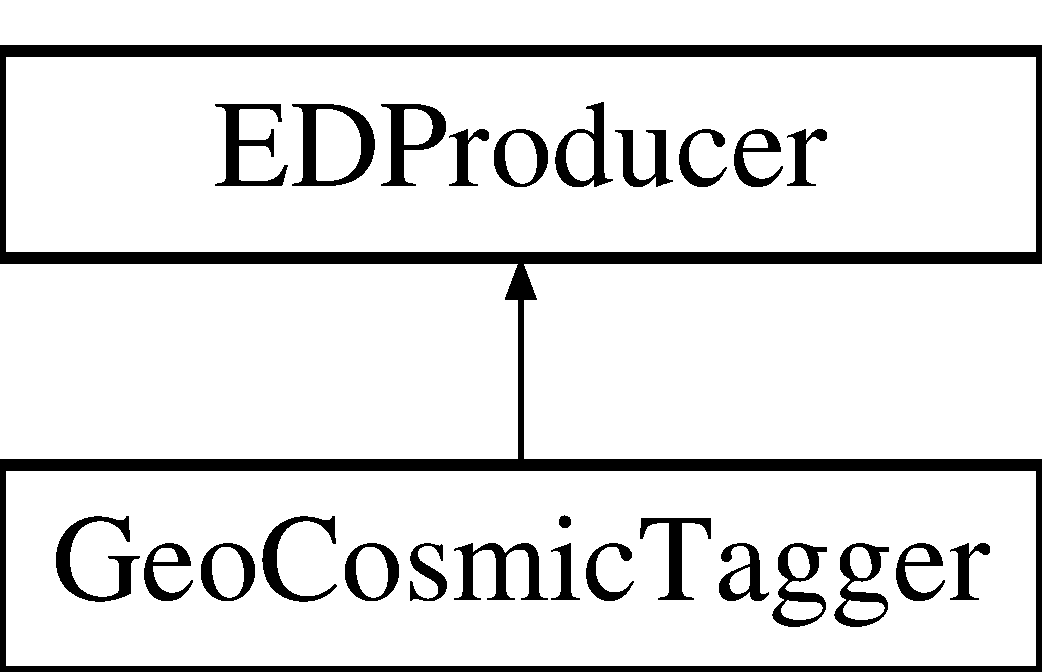
\includegraphics[height=2.000000cm]{classGeoCosmicTagger}
\end{center}
\end{figure}
\subsection*{Public Member Functions}
\begin{DoxyCompactItemize}
\item 
\hypertarget{classGeoCosmicTagger_a7125a3dd08a3a3ec7024f1d31d6968c2}{{\bfseries Geo\-Cosmic\-Tagger} (fhicl\-::\-Parameter\-Set const \&p)}\label{classGeoCosmicTagger_a7125a3dd08a3a3ec7024f1d31d6968c2}

\item 
\hypertarget{classGeoCosmicTagger_a3588400f5291e798c4e294d9f84b4d9a}{{\bfseries Geo\-Cosmic\-Tagger} (\hyperlink{classGeoCosmicTagger}{Geo\-Cosmic\-Tagger} const \&)=delete}\label{classGeoCosmicTagger_a3588400f5291e798c4e294d9f84b4d9a}

\item 
\hypertarget{classGeoCosmicTagger_a4bace9e64488cd816e6dc83a51d0e769}{{\bfseries Geo\-Cosmic\-Tagger} (\hyperlink{classGeoCosmicTagger}{Geo\-Cosmic\-Tagger} \&\&)=delete}\label{classGeoCosmicTagger_a4bace9e64488cd816e6dc83a51d0e769}

\item 
\hypertarget{classGeoCosmicTagger_a9271fbd85d934be890d22402e1bf5bd7}{\hyperlink{classGeoCosmicTagger}{Geo\-Cosmic\-Tagger} \& {\bfseries operator=} (\hyperlink{classGeoCosmicTagger}{Geo\-Cosmic\-Tagger} const \&)=delete}\label{classGeoCosmicTagger_a9271fbd85d934be890d22402e1bf5bd7}

\item 
\hypertarget{classGeoCosmicTagger_a262e77c51ea2288fa59402a4817deea6}{\hyperlink{classGeoCosmicTagger}{Geo\-Cosmic\-Tagger} \& {\bfseries operator=} (\hyperlink{classGeoCosmicTagger}{Geo\-Cosmic\-Tagger} \&\&)=delete}\label{classGeoCosmicTagger_a262e77c51ea2288fa59402a4817deea6}

\item 
\hypertarget{classGeoCosmicTagger_a4683d838f12df03bf06d41d1fcb6fa88}{void {\bfseries produce} (art\-::\-Event \&e) override}\label{classGeoCosmicTagger_a4683d838f12df03bf06d41d1fcb6fa88}

\end{DoxyCompactItemize}


The documentation for this class was generated from the following file\-:\begin{DoxyCompactItemize}
\item 
/home/travis/build/marcodeltutto/\-U\-B\-X\-Sec/\-Modules/Geo\-Cosmic\-Tagger\-\_\-module.\-cc\end{DoxyCompactItemize}

\hypertarget{structubxsec_1_1Hit3D__t}{\section{ubxsec\-:\-:Hit3\-D\-\_\-t Struct Reference}
\label{structubxsec_1_1Hit3D__t}\index{ubxsec\-::\-Hit3\-D\-\_\-t@{ubxsec\-::\-Hit3\-D\-\_\-t}}
}
\subsection*{Public Attributes}
\begin{DoxyCompactItemize}
\item 
\hypertarget{structubxsec_1_1Hit3D__t_ab4929fe0026546ff06fdf001ecfa5b33}{double {\bfseries x}}\label{structubxsec_1_1Hit3D__t_ab4929fe0026546ff06fdf001ecfa5b33}

\item 
\hypertarget{structubxsec_1_1Hit3D__t_ab5462982ffba0961cd4aa3399efac368}{double {\bfseries y}}\label{structubxsec_1_1Hit3D__t_ab5462982ffba0961cd4aa3399efac368}

\item 
\hypertarget{structubxsec_1_1Hit3D__t_a109099e70c1e956e35cf6d4ecab9ef02}{double {\bfseries z}}\label{structubxsec_1_1Hit3D__t_a109099e70c1e956e35cf6d4ecab9ef02}

\item 
\hypertarget{structubxsec_1_1Hit3D__t_a205dc1ee3dba776b70d58809fdc481aa}{double {\bfseries q}}\label{structubxsec_1_1Hit3D__t_a205dc1ee3dba776b70d58809fdc481aa}

\end{DoxyCompactItemize}


The documentation for this struct was generated from the following file\-:\begin{DoxyCompactItemize}
\item 
/home/travis/build/marcodeltutto/\-U\-B\-X\-Sec/\-Modules/U\-B\-X\-Sec\-\_\-module.\-cc\end{DoxyCompactItemize}

\hypertarget{classubana_1_1MCGhost}{\section{ubana\-:\-:M\-C\-Ghost Class Reference}
\label{classubana_1_1MCGhost}\index{ubana\-::\-M\-C\-Ghost@{ubana\-::\-M\-C\-Ghost}}
}


Data product to store a T\-P\-C Object.  




{\ttfamily \#include $<$M\-C\-Ghost.\-h$>$}

\subsection*{Public Member Functions}
\begin{DoxyCompactItemize}
\item 
\hypertarget{classubana_1_1MCGhost_ab78e269293fee8be5b8c6cca432d6d69}{void {\bfseries Set\-Mode} (std\-::string)}\label{classubana_1_1MCGhost_ab78e269293fee8be5b8c6cca432d6d69}

\item 
\hypertarget{classubana_1_1MCGhost_ae6b7f0a7adbf65eb38deb80b3f207f0b}{const std\-::string \& {\bfseries Get\-Mode} () const }\label{classubana_1_1MCGhost_ae6b7f0a7adbf65eb38deb80b3f207f0b}

\end{DoxyCompactItemize}


\subsection{Detailed Description}
Data product to store a T\-P\-C Object. 

\begin{DoxyAuthor}{Author}

\end{DoxyAuthor}
\begin{DoxyParagraph}{Author\-:}
Marco Del Tutto\href{mailto:marco.deltutto@physics.ox.ac.uk}{\tt marco.\-deltutto@physics.\-ox.\-ac.\-uk} 
\end{DoxyParagraph}


\begin{DoxyVersion}{Version}

\end{DoxyVersion}
\begin{DoxyParagraph}{Revision\-:}
1.\-0 
\end{DoxyParagraph}


\begin{DoxyDate}{Date}

\end{DoxyDate}
\begin{DoxyParagraph}{Date\-:}
2017/03/02 
\end{DoxyParagraph}


Contact\-: \href{mailto:marco.deltutto@physics.ox.ac.uk}{\tt marco.\-deltutto@physics.\-ox.\-ac.\-uk}

Created on\-: Friday, May 15, 2017 at 16\-:34\-:34 

The documentation for this class was generated from the following files\-:\begin{DoxyCompactItemize}
\item 
/home/travis/build/marcodeltutto/\-U\-B\-X\-Sec/\-Data\-Types/M\-C\-Ghost.\-h\item 
/home/travis/build/marcodeltutto/\-U\-B\-X\-Sec/\-Data\-Types/M\-C\-Ghost.\-cxx\end{DoxyCompactItemize}

\hypertarget{classMcPfpMatch}{\section{Mc\-Pfp\-Match Class Reference}
\label{classMcPfpMatch}\index{Mc\-Pfp\-Match@{Mc\-Pfp\-Match}}
}


Performs P\-F\-P to M\-C particles match.  




{\ttfamily \#include $<$Mc\-Pfp\-Match.\-h$>$}



\subsection{Detailed Description}
Performs P\-F\-P to M\-C particles match. 

\begin{DoxyAuthor}{Author}

\end{DoxyAuthor}
\begin{DoxyParagraph}{Author\-:}
Marco Del Tutto\href{mailto:marco.deltutto@physics.ox.ac.uk}{\tt marco.\-deltutto@physics.\-ox.\-ac.\-uk} 
\end{DoxyParagraph}


\begin{DoxyVersion}{Version}

\end{DoxyVersion}
\begin{DoxyParagraph}{Revision\-:}
1.\-0 
\end{DoxyParagraph}


\begin{DoxyDate}{Date}

\end{DoxyDate}
\begin{DoxyParagraph}{Date\-:}
2017/03/02 
\end{DoxyParagraph}


Contact\-: \href{mailto:marco.deltutto@physics.ox.ac.uk}{\tt marco.\-deltutto@physics.\-ox.\-ac.\-uk}

Created on\-: Friday, February 03, 2017 at 17\-:24\-:25 Heavily updated on\-: Friday 14, 2017 at 16\-:52\-:41 

The documentation for this class was generated from the following file\-:\begin{DoxyCompactItemize}
\item 
/home/travis/build/marcodeltutto/\-U\-B\-X\-Sec/\-Algorithms/Mc\-Pfp\-Match.\-h\end{DoxyCompactItemize}

\hypertarget{classubxsec_1_1McPfpMatch}{\section{ubxsec\-:\-:Mc\-Pfp\-Match Class Reference}
\label{classubxsec_1_1McPfpMatch}\index{ubxsec\-::\-Mc\-Pfp\-Match@{ubxsec\-::\-Mc\-Pfp\-Match}}
}
\subsection*{Public Member Functions}
\begin{DoxyCompactItemize}
\item 
\hypertarget{classubxsec_1_1McPfpMatch_aea3e9923fdf8855d5798015b36f2d516}{\hyperlink{classubxsec_1_1McPfpMatch_aea3e9923fdf8855d5798015b36f2d516}{Mc\-Pfp\-Match} ()}\label{classubxsec_1_1McPfpMatch_aea3e9923fdf8855d5798015b36f2d516}

\begin{DoxyCompactList}\small\item\em Default constructor. \end{DoxyCompactList}\item 
\hypertarget{classubxsec_1_1McPfpMatch_a3fa822d7321aca21a0ad42e692a29bf2}{\hyperlink{classubxsec_1_1McPfpMatch_a3fa822d7321aca21a0ad42e692a29bf2}{$\sim$\-Mc\-Pfp\-Match} ()}\label{classubxsec_1_1McPfpMatch_a3fa822d7321aca21a0ad42e692a29bf2}

\begin{DoxyCompactList}\small\item\em Default destructor. \end{DoxyCompactList}\item 
\hypertarget{classubxsec_1_1McPfpMatch_aa6578a20f7a8194fae3caa2b19044e40}{void \hyperlink{classubxsec_1_1McPfpMatch_aa6578a20f7a8194fae3caa2b19044e40}{\-\_\-\-Configure\-\_\-} (const Config\-\_\-t \&pset)}\label{classubxsec_1_1McPfpMatch_aa6578a20f7a8194fae3caa2b19044e40}

\begin{DoxyCompactList}\small\item\em Configure. \end{DoxyCompactList}\item 
\hypertarget{classubxsec_1_1McPfpMatch_a15cea806e5a1b12bf2e187d5d26c528d}{void \hyperlink{classubxsec_1_1McPfpMatch_a15cea806e5a1b12bf2e187d5d26c528d}{Configure} (art\-::\-Event const \&e, std\-::string \-\_\-pfp\-\_\-producer, std\-::string \-\_\-spacepoint\-Label, std\-::string \-\_\-hitfinder\-Label, std\-::string \-\_\-geant\-Module\-Label)}\label{classubxsec_1_1McPfpMatch_a15cea806e5a1b12bf2e187d5d26c528d}

\begin{DoxyCompactList}\small\item\em Configure function parameters. \end{DoxyCompactList}\item 
void \hyperlink{classubxsec_1_1McPfpMatch_a1b66ef44f3a1772a4e72de2e5066768c}{Get\-Reco\-To\-True\-Matches} (lar\-\_\-pandora\-::\-M\-C\-Particles\-To\-P\-F\-Particles \&matched\-Particles, lar\-\_\-pandora\-::\-M\-C\-Particles\-To\-Hits \&matched\-Hits)
\begin{DoxyCompactList}\small\item\em Returns matching between true and reconstructed particles. \end{DoxyCompactList}\end{DoxyCompactItemize}
\subsection*{Protected Member Functions}
\begin{DoxyCompactItemize}
\item 
void \hyperlink{classubxsec_1_1McPfpMatch_adb5138d94990f679643372e0be273940}{Get\-Reco\-To\-True\-Matches} (const lar\-\_\-pandora\-::\-P\-F\-Particles\-To\-Hits \&reco\-Particles\-To\-Hits, const lar\-\_\-pandora\-::\-Hits\-To\-M\-C\-Particles \&true\-Hits\-To\-Particles, lar\-\_\-pandora\-::\-M\-C\-Particles\-To\-P\-F\-Particles \&matched\-Particles, lar\-\_\-pandora\-::\-M\-C\-Particles\-To\-Hits \&matched\-Hits)
\begin{DoxyCompactList}\small\item\em Perform matching between true and reconstructed particles. \end{DoxyCompactList}\item 
void \hyperlink{classubxsec_1_1McPfpMatch_a0d41e3e0c60f2777cc26ca8b8520e9d2}{Get\-Reco\-To\-True\-Matches} (const lar\-\_\-pandora\-::\-P\-F\-Particles\-To\-Hits \&reco\-Particles\-To\-Hits, const lar\-\_\-pandora\-::\-Hits\-To\-M\-C\-Particles \&true\-Hits\-To\-Particles, lar\-\_\-pandora\-::\-M\-C\-Particles\-To\-P\-F\-Particles \&matched\-Particles, lar\-\_\-pandora\-::\-M\-C\-Particles\-To\-Hits \&matched\-Hits, P\-F\-Particle\-Set \&reco\-Veto, M\-C\-Particle\-Set \&true\-Veto, bool \-\_\-recursive\-Matching)
\begin{DoxyCompactList}\small\item\em Perform matching between true and reconstructed particles. \end{DoxyCompactList}\end{DoxyCompactItemize}
\subsection*{Protected Attributes}
\begin{DoxyCompactItemize}
\item 
\hypertarget{classubxsec_1_1McPfpMatch_a8e623037c8526c53c0682ba8e42ff62b}{lar\-\_\-pandora\-::\-Hits\-To\-M\-C\-Particles \hyperlink{classubxsec_1_1McPfpMatch_a8e623037c8526c53c0682ba8e42ff62b}{\-\_\-true\-Hits\-To\-Particles}}\label{classubxsec_1_1McPfpMatch_a8e623037c8526c53c0682ba8e42ff62b}

\begin{DoxyCompactList}\small\item\em A map from recon hits to M\-C\-Particles. \end{DoxyCompactList}\item 
\hypertarget{classubxsec_1_1McPfpMatch_a3073567df4d7dca42c95d648ef31cb89}{lar\-\_\-pandora\-::\-P\-F\-Particles\-To\-Hits \hyperlink{classubxsec_1_1McPfpMatch_a3073567df4d7dca42c95d648ef31cb89}{\-\_\-reco\-Particles\-To\-Hits}}\label{classubxsec_1_1McPfpMatch_a3073567df4d7dca42c95d648ef31cb89}

\begin{DoxyCompactList}\small\item\em A map from P\-F\-Particles to recon hits. \end{DoxyCompactList}\end{DoxyCompactItemize}


\subsection{Member Function Documentation}
\hypertarget{classubxsec_1_1McPfpMatch_a1b66ef44f3a1772a4e72de2e5066768c}{\index{ubxsec\-::\-Mc\-Pfp\-Match@{ubxsec\-::\-Mc\-Pfp\-Match}!Get\-Reco\-To\-True\-Matches@{Get\-Reco\-To\-True\-Matches}}
\index{Get\-Reco\-To\-True\-Matches@{Get\-Reco\-To\-True\-Matches}!ubxsec::McPfpMatch@{ubxsec\-::\-Mc\-Pfp\-Match}}
\subsubsection[{Get\-Reco\-To\-True\-Matches}]{\setlength{\rightskip}{0pt plus 5cm}void Mc\-Pfp\-Match\-::\-Get\-Reco\-To\-True\-Matches (
\begin{DoxyParamCaption}
\item[{lar\-\_\-pandora\-::\-M\-C\-Particles\-To\-P\-F\-Particles \&}]{matched\-Particles, }
\item[{lar\-\_\-pandora\-::\-M\-C\-Particles\-To\-Hits \&}]{matched\-Hits}
\end{DoxyParamCaption}
)}}\label{classubxsec_1_1McPfpMatch_a1b66ef44f3a1772a4e72de2e5066768c}


Returns matching between true and reconstructed particles. 


\begin{DoxyParams}{Parameters}
{\em matched\-Particles} & the output matches between reconstructed and true particles \\
\hline
{\em matched\-Hits} & the output matches between reconstructed particles and hits \\
\hline
\end{DoxyParams}
\hypertarget{classubxsec_1_1McPfpMatch_adb5138d94990f679643372e0be273940}{\index{ubxsec\-::\-Mc\-Pfp\-Match@{ubxsec\-::\-Mc\-Pfp\-Match}!Get\-Reco\-To\-True\-Matches@{Get\-Reco\-To\-True\-Matches}}
\index{Get\-Reco\-To\-True\-Matches@{Get\-Reco\-To\-True\-Matches}!ubxsec::McPfpMatch@{ubxsec\-::\-Mc\-Pfp\-Match}}
\subsubsection[{Get\-Reco\-To\-True\-Matches}]{\setlength{\rightskip}{0pt plus 5cm}void Mc\-Pfp\-Match\-::\-Get\-Reco\-To\-True\-Matches (
\begin{DoxyParamCaption}
\item[{const lar\-\_\-pandora\-::\-P\-F\-Particles\-To\-Hits \&}]{reco\-Particles\-To\-Hits, }
\item[{const lar\-\_\-pandora\-::\-Hits\-To\-M\-C\-Particles \&}]{true\-Hits\-To\-Particles, }
\item[{lar\-\_\-pandora\-::\-M\-C\-Particles\-To\-P\-F\-Particles \&}]{matched\-Particles, }
\item[{lar\-\_\-pandora\-::\-M\-C\-Particles\-To\-Hits \&}]{matched\-Hits}
\end{DoxyParamCaption}
)\hspace{0.3cm}{\ttfamily [protected]}}}\label{classubxsec_1_1McPfpMatch_adb5138d94990f679643372e0be273940}


Perform matching between true and reconstructed particles. 


\begin{DoxyParams}{Parameters}
{\em reco\-Particles\-To\-Hits} & the mapping from reconstructed particles to hits \\
\hline
{\em true\-Hits\-To\-Particles} & the mapping from hits to true particles \\
\hline
{\em matched\-Particles} & the output matches between reconstructed and true particles \\
\hline
{\em matched\-Hits} & the output matches between reconstructed particles and hits \\
\hline
\end{DoxyParams}
\hypertarget{classubxsec_1_1McPfpMatch_a0d41e3e0c60f2777cc26ca8b8520e9d2}{\index{ubxsec\-::\-Mc\-Pfp\-Match@{ubxsec\-::\-Mc\-Pfp\-Match}!Get\-Reco\-To\-True\-Matches@{Get\-Reco\-To\-True\-Matches}}
\index{Get\-Reco\-To\-True\-Matches@{Get\-Reco\-To\-True\-Matches}!ubxsec::McPfpMatch@{ubxsec\-::\-Mc\-Pfp\-Match}}
\subsubsection[{Get\-Reco\-To\-True\-Matches}]{\setlength{\rightskip}{0pt plus 5cm}void Mc\-Pfp\-Match\-::\-Get\-Reco\-To\-True\-Matches (
\begin{DoxyParamCaption}
\item[{const lar\-\_\-pandora\-::\-P\-F\-Particles\-To\-Hits \&}]{reco\-Particles\-To\-Hits, }
\item[{const lar\-\_\-pandora\-::\-Hits\-To\-M\-C\-Particles \&}]{true\-Hits\-To\-Particles, }
\item[{lar\-\_\-pandora\-::\-M\-C\-Particles\-To\-P\-F\-Particles \&}]{matched\-Particles, }
\item[{lar\-\_\-pandora\-::\-M\-C\-Particles\-To\-Hits \&}]{matched\-Hits, }
\item[{P\-F\-Particle\-Set \&}]{reco\-Veto, }
\item[{M\-C\-Particle\-Set \&}]{true\-Veto, }
\item[{bool}]{\-\_\-recursive\-Matching}
\end{DoxyParamCaption}
)\hspace{0.3cm}{\ttfamily [protected]}}}\label{classubxsec_1_1McPfpMatch_a0d41e3e0c60f2777cc26ca8b8520e9d2}


Perform matching between true and reconstructed particles. 


\begin{DoxyParams}{Parameters}
{\em reco\-Particles\-To\-Hits} & the mapping from reconstructed particles to hits \\
\hline
{\em true\-Hits\-To\-Particles} & the mapping from hits to true particles \\
\hline
{\em matched\-Particles} & the output matches between reconstructed and true particles \\
\hline
{\em matched\-Hits} & the output matches between reconstructed particles and hits \\
\hline
{\em reco\-Veto} & the veto list for reconstructed particles \\
\hline
{\em true\-Veto} & the veto list for true particles \\
\hline
\end{DoxyParams}


The documentation for this class was generated from the following files\-:\begin{DoxyCompactItemize}
\item 
/home/travis/build/marcodeltutto/\-U\-B\-X\-Sec/\-Algorithms/Mc\-Pfp\-Match.\-h\item 
/home/travis/build/marcodeltutto/\-U\-B\-X\-Sec/\-Algorithms/Mc\-Pfp\-Match.\-cxx\end{DoxyCompactItemize}

\hypertarget{classubana_1_1MuonCandidateFinder}{\section{ubana\-:\-:Muon\-Candidate\-Finder Class Reference}
\label{classubana_1_1MuonCandidateFinder}\index{ubana\-::\-Muon\-Candidate\-Finder@{ubana\-::\-Muon\-Candidate\-Finder}}
}


{\ttfamily \#include $<$Muon\-Candidate\-Finder.\-h$>$}

\subsection*{Public Member Functions}
\begin{DoxyCompactItemize}
\item 
\hypertarget{classubana_1_1MuonCandidateFinder_a6dff5780726e46fc5ad43f41bdbc0a97}{\hyperlink{classubana_1_1MuonCandidateFinder_a6dff5780726e46fc5ad43f41bdbc0a97}{Muon\-Candidate\-Finder} ()}\label{classubana_1_1MuonCandidateFinder_a6dff5780726e46fc5ad43f41bdbc0a97}

\begin{DoxyCompactList}\small\item\em Default constructor. \end{DoxyCompactList}\item 
\hypertarget{classubana_1_1MuonCandidateFinder_aa84c2c422211c74d00eb61cc221d8c07}{\hyperlink{classubana_1_1MuonCandidateFinder_aa84c2c422211c74d00eb61cc221d8c07}{$\sim$\-Muon\-Candidate\-Finder} ()}\label{classubana_1_1MuonCandidateFinder_aa84c2c422211c74d00eb61cc221d8c07}

\begin{DoxyCompactList}\small\item\em Default destructor. \end{DoxyCompactList}\item 
\hypertarget{classubana_1_1MuonCandidateFinder_a97d58ef9b5d26a6ccddc18f507ada1b1}{void \hyperlink{classubana_1_1MuonCandidateFinder_a97d58ef9b5d26a6ccddc18f507ada1b1}{Configure} (fhicl\-::\-Parameter\-Set const \&p)}\label{classubana_1_1MuonCandidateFinder_a97d58ef9b5d26a6ccddc18f507ada1b1}

\begin{DoxyCompactList}\small\item\em Configure function parameters. \end{DoxyCompactList}\item 
\hypertarget{classubana_1_1MuonCandidateFinder_ae5aaa85fb815cd30fe1048ea5cdd387d}{void \hyperlink{classubana_1_1MuonCandidateFinder_ae5aaa85fb815cd30fe1048ea5cdd387d}{Print\-Config} ()}\label{classubana_1_1MuonCandidateFinder_ae5aaa85fb815cd30fe1048ea5cdd387d}

\begin{DoxyCompactList}\small\item\em Print the current configuration. \end{DoxyCompactList}\item 
\hypertarget{classubana_1_1MuonCandidateFinder_a1cdd1745117a85bbcfc1de5167c7e688}{void \hyperlink{classubana_1_1MuonCandidateFinder_a1cdd1745117a85bbcfc1de5167c7e688}{Set\-Tracks} (std\-::vector$<$ art\-::\-Ptr$<$ recob\-::\-Track $>$$>$ thetracks)}\label{classubana_1_1MuonCandidateFinder_a1cdd1745117a85bbcfc1de5167c7e688}

\begin{DoxyCompactList}\small\item\em Set the tracks. \end{DoxyCompactList}\item 
\hypertarget{classubana_1_1MuonCandidateFinder_adc3333300fec98b692ff12550c3d8d53}{void \hyperlink{classubana_1_1MuonCandidateFinder_adc3333300fec98b692ff12550c3d8d53}{Set\-Track\-To\-P\-I\-D\-Map} (std\-::map$<$ art\-::\-Ptr$<$ recob\-::\-Track $>$, art\-::\-Ptr$<$ anab\-::\-Particle\-I\-D $>$$>$ themap)}\label{classubana_1_1MuonCandidateFinder_adc3333300fec98b692ff12550c3d8d53}

\begin{DoxyCompactList}\small\item\em Set map from tracks to P\-I\-D for the T\-P\-C object. \end{DoxyCompactList}\item 
\hypertarget{classubana_1_1MuonCandidateFinder_a8f852194c03bf0b3c04650850271c7d9}{bool \hyperlink{classubana_1_1MuonCandidateFinder_a8f852194c03bf0b3c04650850271c7d9}{Get\-Candidate\-Track} (art\-::\-Ptr$<$ recob\-::\-Track $>$ \&)}\label{classubana_1_1MuonCandidateFinder_a8f852194c03bf0b3c04650850271c7d9}

\begin{DoxyCompactList}\small\item\em Sets the T\-P\-C object. \end{DoxyCompactList}\end{DoxyCompactItemize}
\subsection*{Protected Attributes}
\begin{DoxyCompactItemize}
\item 
\hypertarget{classubana_1_1MuonCandidateFinder_aa7c96f8b784bcd81512e9c444806f740}{std\-::vector$<$ art\-::\-Ptr\\*
$<$ recob\-::\-Track $>$ $>$ {\bfseries \-\_\-tracks}}\label{classubana_1_1MuonCandidateFinder_aa7c96f8b784bcd81512e9c444806f740}

\item 
\hypertarget{classubana_1_1MuonCandidateFinder_a673e9b7d68a2c3c734fd92ec6e0a87ee}{std\-::map$<$ art\-::\-Ptr\\*
$<$ recob\-::\-Track $>$, art\-::\-Ptr\\*
$<$ anab\-::\-Particle\-I\-D $>$ $>$ {\bfseries \-\_\-track\-\_\-to\-\_\-pid}}\label{classubana_1_1MuonCandidateFinder_a673e9b7d68a2c3c734fd92ec6e0a87ee}

\item 
\hypertarget{classubana_1_1MuonCandidateFinder_a4f0eef92dcbab86d2470da30739be235}{bool {\bfseries \-\_\-use\-\_\-pida\-\_\-cut}}\label{classubana_1_1MuonCandidateFinder_a4f0eef92dcbab86d2470da30739be235}

\item 
\hypertarget{classubana_1_1MuonCandidateFinder_a7275929ef39e422785e7a6dd9d95f5eb}{bool {\bfseries \-\_\-tracks\-\_\-are\-\_\-set}}\label{classubana_1_1MuonCandidateFinder_a7275929ef39e422785e7a6dd9d95f5eb}

\item 
\hypertarget{classubana_1_1MuonCandidateFinder_a46cb4b649e6d2d9b2e6c7641a9fd548a}{bool {\bfseries \-\_\-tracktopidmap\-\_\-is\-\_\-set}}\label{classubana_1_1MuonCandidateFinder_a46cb4b649e6d2d9b2e6c7641a9fd548a}

\end{DoxyCompactItemize}


\subsection{Detailed Description}
User defined class \hyperlink{classubana_1_1MuonCandidateFinder}{Muon\-Candidate\-Finder} ... these comments are used to generate doxygen documentation! 

The documentation for this class was generated from the following files\-:\begin{DoxyCompactItemize}
\item 
/home/travis/build/marcodeltutto/\-U\-B\-X\-Sec/\-Algorithms/\hyperlink{MuonCandidateFinder_8h}{Muon\-Candidate\-Finder.\-h}\item 
/home/travis/build/marcodeltutto/\-U\-B\-X\-Sec/\-Algorithms/Muon\-Candidate\-Finder.\-cxx\end{DoxyCompactItemize}

\hypertarget{classNeutrinoFlashMatch}{\section{Neutrino\-Flash\-Match Class Reference}
\label{classNeutrinoFlashMatch}\index{Neutrino\-Flash\-Match@{Neutrino\-Flash\-Match}}
}
Inheritance diagram for Neutrino\-Flash\-Match\-:\begin{figure}[H]
\begin{center}
\leavevmode
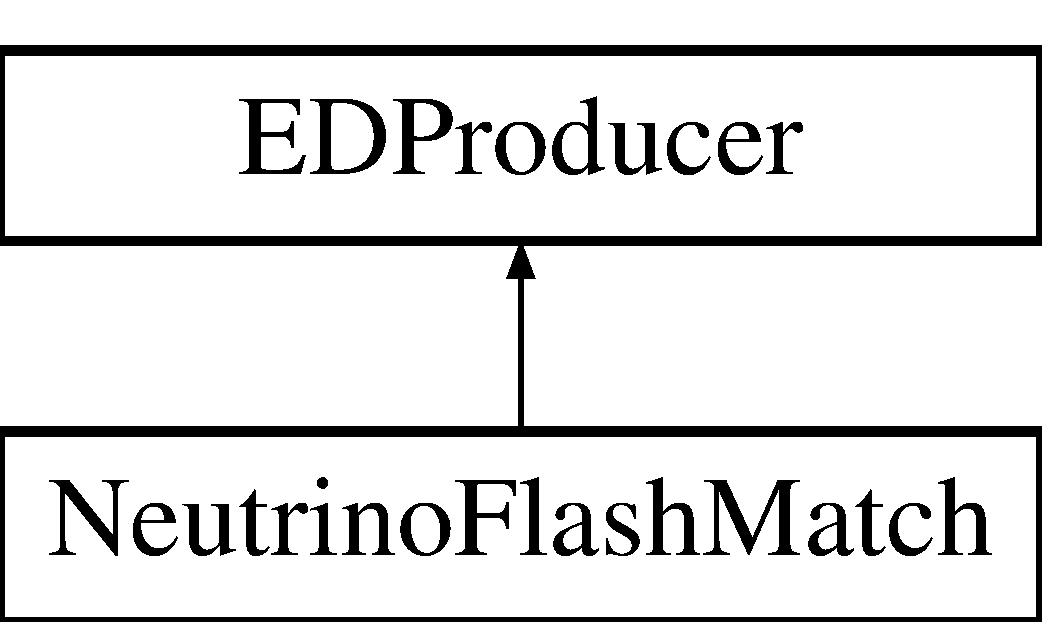
\includegraphics[height=2.000000cm]{classNeutrinoFlashMatch}
\end{center}
\end{figure}
\subsection*{Public Member Functions}
\begin{DoxyCompactItemize}
\item 
\hypertarget{classNeutrinoFlashMatch_a2c3aa4e9461e3f31e9d198ba5d481cd6}{{\bfseries Neutrino\-Flash\-Match} (fhicl\-::\-Parameter\-Set const \&p)}\label{classNeutrinoFlashMatch_a2c3aa4e9461e3f31e9d198ba5d481cd6}

\item 
\hypertarget{classNeutrinoFlashMatch_af69b13e9ca68fff69d3e9d8280d9c436}{{\bfseries Neutrino\-Flash\-Match} (\hyperlink{classNeutrinoFlashMatch}{Neutrino\-Flash\-Match} const \&)=delete}\label{classNeutrinoFlashMatch_af69b13e9ca68fff69d3e9d8280d9c436}

\item 
\hypertarget{classNeutrinoFlashMatch_a5e58dc2e3e587db95317151b1acd6518}{{\bfseries Neutrino\-Flash\-Match} (\hyperlink{classNeutrinoFlashMatch}{Neutrino\-Flash\-Match} \&\&)=delete}\label{classNeutrinoFlashMatch_a5e58dc2e3e587db95317151b1acd6518}

\item 
\hypertarget{classNeutrinoFlashMatch_afd7be5fa45629eca0b992c8d31adc747}{\hyperlink{classNeutrinoFlashMatch}{Neutrino\-Flash\-Match} \& {\bfseries operator=} (\hyperlink{classNeutrinoFlashMatch}{Neutrino\-Flash\-Match} const \&)=delete}\label{classNeutrinoFlashMatch_afd7be5fa45629eca0b992c8d31adc747}

\item 
\hypertarget{classNeutrinoFlashMatch_ac1b32943963d8f7f50339410dbdcfd5c}{\hyperlink{classNeutrinoFlashMatch}{Neutrino\-Flash\-Match} \& {\bfseries operator=} (\hyperlink{classNeutrinoFlashMatch}{Neutrino\-Flash\-Match} \&\&)=delete}\label{classNeutrinoFlashMatch_ac1b32943963d8f7f50339410dbdcfd5c}

\item 
\hypertarget{classNeutrinoFlashMatch_aa511b92472bb70883c5a666293be1da3}{flashana\-::\-Q\-Cluster\-\_\-t \hyperlink{classNeutrinoFlashMatch_aa511b92472bb70883c5a666293be1da3}{Get\-Q\-Cluster} (std\-::vector$<$ art\-::\-Ptr$<$ recob\-::\-Track $>$$>$)}\label{classNeutrinoFlashMatch_aa511b92472bb70883c5a666293be1da3}

\begin{DoxyCompactList}\small\item\em Takes a vector of recob\-::\-Tracks and returns a Q\-Cluster made out from all the tracks in the vector. \end{DoxyCompactList}\item 
\hypertarget{classNeutrinoFlashMatch_a93132a117b6ea907ba95bba4a6af6107}{flashana\-::\-Q\-Cluster\-\_\-t \hyperlink{classNeutrinoFlashMatch_a93132a117b6ea907ba95bba4a6af6107}{Get\-Q\-Cluster} (std\-::vector$<$ art\-::\-Ptr$<$ recob\-::\-P\-F\-Particle $>$$>$, lar\-\_\-pandora\-::\-P\-F\-Particles\-To\-Space\-Points pfp\-\_\-to\-\_\-spacept, lar\-\_\-pandora\-::\-Space\-Points\-To\-Hits spacept\-\_\-to\-\_\-hits)}\label{classNeutrinoFlashMatch_a93132a117b6ea907ba95bba4a6af6107}

\begin{DoxyCompactList}\small\item\em Takes a vector of recob\-::\-P\-F\-Particle and two maps and returns a Q\-Cluster made out from all the tracks in the vector (test) \end{DoxyCompactList}\item 
\hypertarget{classNeutrinoFlashMatch_aa957152a8c232e4b23cc7544aa6bfdd1}{flashana\-::\-Flash\-\_\-t \hyperlink{classNeutrinoFlashMatch_aa957152a8c232e4b23cc7544aa6bfdd1}{Trial} (std\-::vector$<$ art\-::\-Ptr$<$ recob\-::\-Track $>$$>$ track\-\_\-v, flashana\-::\-Flash\-\_\-t flash\-Beam, double \&\-\_\-chi2, double \&\-\_\-ll)}\label{classNeutrinoFlashMatch_aa957152a8c232e4b23cc7544aa6bfdd1}

\begin{DoxyCompactList}\small\item\em Test method to calculate the flash-\/\-T\-P\-Cobject compatibilty at a fixed x position. \end{DoxyCompactList}\item 
\hypertarget{classNeutrinoFlashMatch_a00578af5672ff925f80c1b9482c8b4ff}{void {\bfseries produce} (art\-::\-Event \&e) override}\label{classNeutrinoFlashMatch_a00578af5672ff925f80c1b9482c8b4ff}

\end{DoxyCompactItemize}


The documentation for this class was generated from the following file\-:\begin{DoxyCompactItemize}
\item 
/home/travis/build/marcodeltutto/\-U\-B\-X\-Sec/\-Modules/Neutrino\-Flash\-Match\-\_\-module.\-cc\end{DoxyCompactItemize}

\hypertarget{classNeutrinoMCFlash}{\section{Neutrino\-M\-C\-Flash Class Reference}
\label{classNeutrinoMCFlash}\index{Neutrino\-M\-C\-Flash@{Neutrino\-M\-C\-Flash}}
}
Inheritance diagram for Neutrino\-M\-C\-Flash\-:\begin{figure}[H]
\begin{center}
\leavevmode
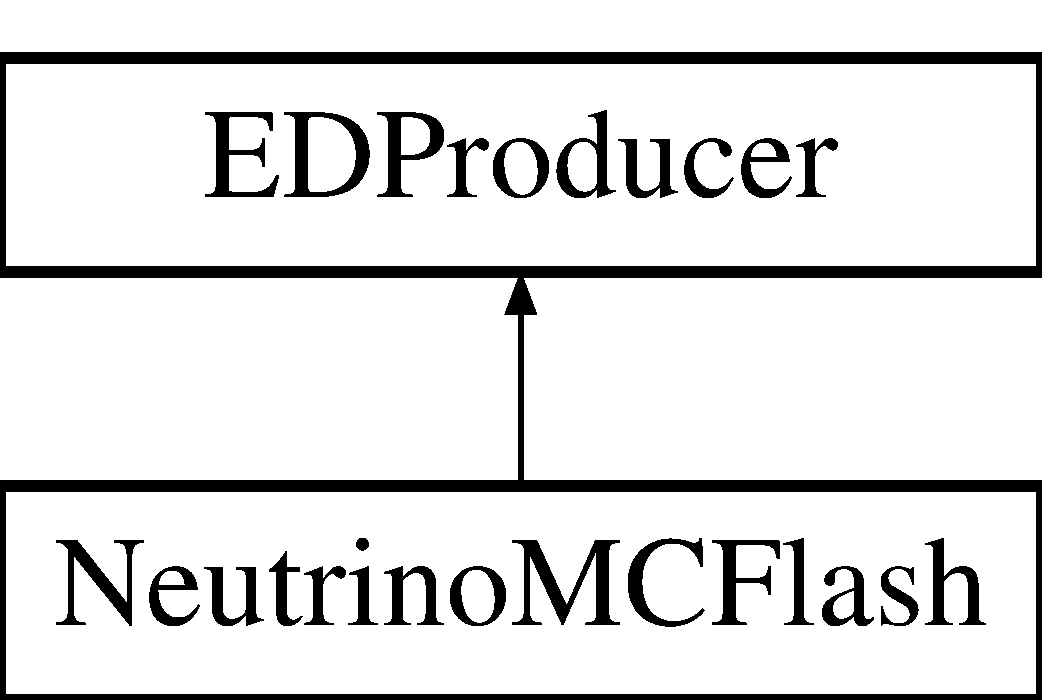
\includegraphics[height=2.000000cm]{classNeutrinoMCFlash}
\end{center}
\end{figure}
\subsection*{Public Member Functions}
\begin{DoxyCompactItemize}
\item 
\hypertarget{classNeutrinoMCFlash_a924c91e62abb544113c57f337b792da0}{{\bfseries Neutrino\-M\-C\-Flash} (fhicl\-::\-Parameter\-Set const \&p)}\label{classNeutrinoMCFlash_a924c91e62abb544113c57f337b792da0}

\item 
\hypertarget{classNeutrinoMCFlash_a1c2730ddb25b20ea1888ecab79b5d08b}{{\bfseries Neutrino\-M\-C\-Flash} (\hyperlink{classNeutrinoMCFlash}{Neutrino\-M\-C\-Flash} const \&)=delete}\label{classNeutrinoMCFlash_a1c2730ddb25b20ea1888ecab79b5d08b}

\item 
\hypertarget{classNeutrinoMCFlash_aaa3156265c398dcf28e2f89221010ba4}{{\bfseries Neutrino\-M\-C\-Flash} (\hyperlink{classNeutrinoMCFlash}{Neutrino\-M\-C\-Flash} \&\&)=delete}\label{classNeutrinoMCFlash_aaa3156265c398dcf28e2f89221010ba4}

\item 
\hypertarget{classNeutrinoMCFlash_a4473e1b794f33fde6aea4c741a5ebeda}{\hyperlink{classNeutrinoMCFlash}{Neutrino\-M\-C\-Flash} \& {\bfseries operator=} (\hyperlink{classNeutrinoMCFlash}{Neutrino\-M\-C\-Flash} const \&)=delete}\label{classNeutrinoMCFlash_a4473e1b794f33fde6aea4c741a5ebeda}

\item 
\hypertarget{classNeutrinoMCFlash_a13f1fc3b336ec7c9bd96983ec51b3e22}{\hyperlink{classNeutrinoMCFlash}{Neutrino\-M\-C\-Flash} \& {\bfseries operator=} (\hyperlink{classNeutrinoMCFlash}{Neutrino\-M\-C\-Flash} \&\&)=delete}\label{classNeutrinoMCFlash_a13f1fc3b336ec7c9bd96983ec51b3e22}

\item 
\hypertarget{classNeutrinoMCFlash_a96fff468ffb1b1182b296d9bdab6d31b}{void {\bfseries produce} (art\-::\-Event \&e) override}\label{classNeutrinoMCFlash_a96fff468ffb1b1182b296d9bdab6d31b}

\end{DoxyCompactItemize}


The documentation for this class was generated from the following file\-:\begin{DoxyCompactItemize}
\item 
/home/travis/build/marcodeltutto/\-U\-B\-X\-Sec/\-Modules/Neutrino\-M\-C\-Flash\-\_\-module.\-cc\end{DoxyCompactItemize}

\hypertarget{classubana_1_1NuMuCCEventSelection}{\section{ubana\-:\-:Nu\-Mu\-C\-C\-Event\-Selection Class Reference}
\label{classubana_1_1NuMuCCEventSelection}\index{ubana\-::\-Nu\-Mu\-C\-C\-Event\-Selection@{ubana\-::\-Nu\-Mu\-C\-C\-Event\-Selection}}
}


{\ttfamily \#include $<$Nu\-Mu\-C\-C\-Event\-Selection.\-h$>$}

\subsection*{Public Member Functions}
\begin{DoxyCompactItemize}
\item 
\hypertarget{classubana_1_1NuMuCCEventSelection_a8c96431500a98d4493a70dc715f3d00d}{\hyperlink{classubana_1_1NuMuCCEventSelection_a8c96431500a98d4493a70dc715f3d00d}{Nu\-Mu\-C\-C\-Event\-Selection} ()}\label{classubana_1_1NuMuCCEventSelection_a8c96431500a98d4493a70dc715f3d00d}

\begin{DoxyCompactList}\small\item\em Default constructor. \end{DoxyCompactList}\item 
\hypertarget{classubana_1_1NuMuCCEventSelection_a02e9e44da798b1ab984e373abf6fb795}{\hyperlink{classubana_1_1NuMuCCEventSelection_a02e9e44da798b1ab984e373abf6fb795}{$\sim$\-Nu\-Mu\-C\-C\-Event\-Selection} ()}\label{classubana_1_1NuMuCCEventSelection_a02e9e44da798b1ab984e373abf6fb795}

\begin{DoxyCompactList}\small\item\em Default destructor. \end{DoxyCompactList}\item 
\hypertarget{classubana_1_1NuMuCCEventSelection_a8395dc0a9642df63c192feccd24265f2}{void \hyperlink{classubana_1_1NuMuCCEventSelection_a8395dc0a9642df63c192feccd24265f2}{Configure} (fhicl\-::\-Parameter\-Set const \&p)}\label{classubana_1_1NuMuCCEventSelection_a8395dc0a9642df63c192feccd24265f2}

\begin{DoxyCompactList}\small\item\em Configure function parameters. \end{DoxyCompactList}\item 
\hypertarget{classubana_1_1NuMuCCEventSelection_a25fadae27bbb94bcdd86a11564c47be9}{void \hyperlink{classubana_1_1NuMuCCEventSelection_a25fadae27bbb94bcdd86a11564c47be9}{Print\-Config} ()}\label{classubana_1_1NuMuCCEventSelection_a25fadae27bbb94bcdd86a11564c47be9}

\begin{DoxyCompactList}\small\item\em Print the current configuration. \end{DoxyCompactList}\item 
\hypertarget{classubana_1_1NuMuCCEventSelection_aab2612c63b22127e3d3909c8fdd8b9b7}{void \hyperlink{classubana_1_1NuMuCCEventSelection_aab2612c63b22127e3d3909c8fdd8b9b7}{Set\-Event} (\hyperlink{classUBXSecEvent}{U\-B\-X\-Sec\-Event} $\ast$)}\label{classubana_1_1NuMuCCEventSelection_aab2612c63b22127e3d3909c8fdd8b9b7}

\begin{DoxyCompactList}\small\item\em Set the \hyperlink{classUBXSecEvent}{U\-B\-X\-Sec\-Event}. \end{DoxyCompactList}\item 
\hypertarget{classubana_1_1NuMuCCEventSelection_af1fce817e5534d638d2a18fbc6ce25dd}{bool \hyperlink{classubana_1_1NuMuCCEventSelection_af1fce817e5534d638d2a18fbc6ce25dd}{Is\-Selected} (size\-\_\-t \&slice\-\_\-index, std\-::map$<$ std\-::string, bool $>$ \&failure\-\_\-map)}\label{classubana_1_1NuMuCCEventSelection_af1fce817e5534d638d2a18fbc6ce25dd}

\begin{DoxyCompactList}\small\item\em Returns true if this event is selected. \end{DoxyCompactList}\end{DoxyCompactItemize}
\subsection*{Protected Attributes}
\begin{DoxyCompactItemize}
\item 
\hypertarget{classubana_1_1NuMuCCEventSelection_a48de2fddcc05d0908fde350554f35a88}{\hyperlink{classUBXSecEvent}{U\-B\-X\-Sec\-Event} $\ast$ {\bfseries \-\_\-ubxsec\-\_\-event}}\label{classubana_1_1NuMuCCEventSelection_a48de2fddcc05d0908fde350554f35a88}

\item 
\hypertarget{classubana_1_1NuMuCCEventSelection_adf35ca6074630cd6a6ebd5c68796008f}{bool {\bfseries \-\_\-event\-\_\-is\-\_\-set} = false}\label{classubana_1_1NuMuCCEventSelection_adf35ca6074630cd6a6ebd5c68796008f}

\item 
\hypertarget{classubana_1_1NuMuCCEventSelection_a4a5892657ab7f3cd6f459b44653cc379}{bool {\bfseries \-\_\-configured} = false}\label{classubana_1_1NuMuCCEventSelection_a4a5892657ab7f3cd6f459b44653cc379}

\item 
\hypertarget{classubana_1_1NuMuCCEventSelection_a7fe39da04269f48dfa309f9785b27fd4}{bool {\bfseries \-\_\-verbose}}\label{classubana_1_1NuMuCCEventSelection_a7fe39da04269f48dfa309f9785b27fd4}

\item 
\hypertarget{classubana_1_1NuMuCCEventSelection_a006ec45816b44b43f9711b4ba872f15a}{double {\bfseries \-\_\-deltax\-\_\-cut\-\_\-down}}\label{classubana_1_1NuMuCCEventSelection_a006ec45816b44b43f9711b4ba872f15a}

\item 
\hypertarget{classubana_1_1NuMuCCEventSelection_a9c8ca172c06c9d209a2d061bf8aee2dc}{double {\bfseries \-\_\-deltax\-\_\-cut\-\_\-up}}\label{classubana_1_1NuMuCCEventSelection_a9c8ca172c06c9d209a2d061bf8aee2dc}

\item 
\hypertarget{classubana_1_1NuMuCCEventSelection_acabd030a01171b65371ba3fe15dd549c}{double {\bfseries \-\_\-deltaz\-\_\-cut\-\_\-down}}\label{classubana_1_1NuMuCCEventSelection_acabd030a01171b65371ba3fe15dd549c}

\item 
\hypertarget{classubana_1_1NuMuCCEventSelection_ac070028424ca4d45b6f34e1783190bbd}{double {\bfseries \-\_\-deltaz\-\_\-cut\-\_\-up}}\label{classubana_1_1NuMuCCEventSelection_ac070028424ca4d45b6f34e1783190bbd}

\item 
\hypertarget{classubana_1_1NuMuCCEventSelection_ab3b2bd085e4d94041d4606004e7e7c84}{double {\bfseries \-\_\-flsmatch\-\_\-score\-\_\-cut}}\label{classubana_1_1NuMuCCEventSelection_ab3b2bd085e4d94041d4606004e7e7c84}

\item 
\hypertarget{classubana_1_1NuMuCCEventSelection_ab3d603d87565634367e9c1b0a432e768}{double {\bfseries \-\_\-vtxcheck\-\_\-angle\-\_\-cut\-\_\-down}}\label{classubana_1_1NuMuCCEventSelection_ab3d603d87565634367e9c1b0a432e768}

\item 
\hypertarget{classubana_1_1NuMuCCEventSelection_aecedda900c5db3ae97a2a56d2b2ca0ce}{double {\bfseries \-\_\-vtxcheck\-\_\-angle\-\_\-cut\-\_\-up}}\label{classubana_1_1NuMuCCEventSelection_aecedda900c5db3ae97a2a56d2b2ca0ce}

\item 
\hypertarget{classubana_1_1NuMuCCEventSelection_a1b57d12027f73b53cfd959f041854891}{double {\bfseries \-\_\-mcs\-\_\-length\-\_\-cut}}\label{classubana_1_1NuMuCCEventSelection_a1b57d12027f73b53cfd959f041854891}

\item 
\hypertarget{classubana_1_1NuMuCCEventSelection_aedd8196829ba2459ec0cf3784f67bcb9}{double {\bfseries \-\_\-ntrack\-\_\-cut}}\label{classubana_1_1NuMuCCEventSelection_aedd8196829ba2459ec0cf3784f67bcb9}

\item 
\hypertarget{classubana_1_1NuMuCCEventSelection_abad9fc8197e1d13ee7f35551cedeacaa}{double {\bfseries \-\_\-pe\-\_\-cut}}\label{classubana_1_1NuMuCCEventSelection_abad9fc8197e1d13ee7f35551cedeacaa}

\item 
\hypertarget{classubana_1_1NuMuCCEventSelection_af08a0c70e21fbef10efd34dde2fe7d83}{double {\bfseries \-\_\-beam\-Spill\-Starts}}\label{classubana_1_1NuMuCCEventSelection_af08a0c70e21fbef10efd34dde2fe7d83}

\item 
\hypertarget{classubana_1_1NuMuCCEventSelection_a2a52cfd60173c161bf9169cf26964eea}{double {\bfseries \-\_\-beam\-Spill\-Ends}}\label{classubana_1_1NuMuCCEventSelection_a2a52cfd60173c161bf9169cf26964eea}

\end{DoxyCompactItemize}


\subsection{Detailed Description}
User defined class \hyperlink{classubana_1_1NuMuCCEventSelection}{Nu\-Mu\-C\-C\-Event\-Selection} ... these comments are used to generate doxygen documentation! 

The documentation for this class was generated from the following files\-:\begin{DoxyCompactItemize}
\item 
/home/travis/build/marcodeltutto/\-U\-B\-X\-Sec/\-Algorithms/\hyperlink{NuMuCCEventSelection_8h}{Nu\-Mu\-C\-C\-Event\-Selection.\-h}\item 
/home/travis/build/marcodeltutto/\-U\-B\-X\-Sec/\-Algorithms/Nu\-Mu\-C\-C\-Event\-Selection.\-cxx\end{DoxyCompactItemize}

\hypertarget{classPhotonActivity}{\section{Photon\-Activity Class Reference}
\label{classPhotonActivity}\index{Photon\-Activity@{Photon\-Activity}}
}
Inheritance diagram for Photon\-Activity\-:\begin{figure}[H]
\begin{center}
\leavevmode
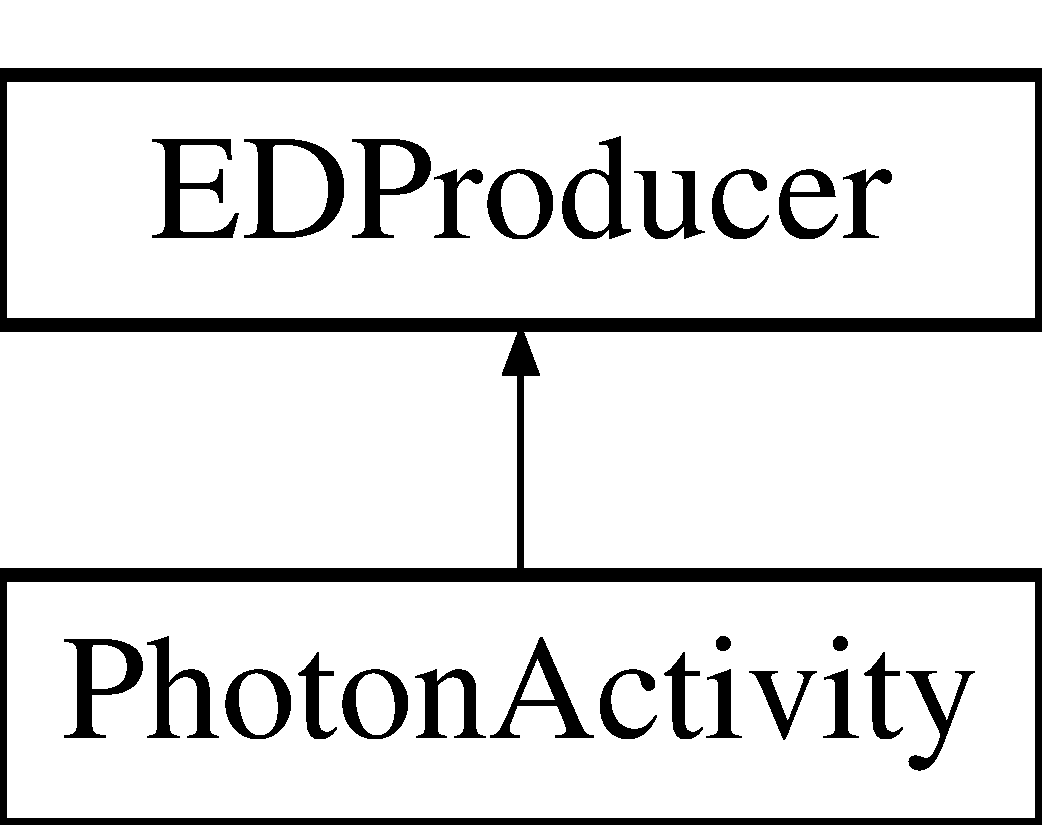
\includegraphics[height=2.000000cm]{classPhotonActivity}
\end{center}
\end{figure}
\subsection*{Public Member Functions}
\begin{DoxyCompactItemize}
\item 
\hypertarget{classPhotonActivity_a76dfd63b90435e0b7ec3b74ee15f7ac2}{{\bfseries Photon\-Activity} (fhicl\-::\-Parameter\-Set const \&p)}\label{classPhotonActivity_a76dfd63b90435e0b7ec3b74ee15f7ac2}

\item 
\hypertarget{classPhotonActivity_ac57409a0d4ddb84c398cb1f48e0be2ba}{{\bfseries Photon\-Activity} (\hyperlink{classPhotonActivity}{Photon\-Activity} const \&)=delete}\label{classPhotonActivity_ac57409a0d4ddb84c398cb1f48e0be2ba}

\item 
\hypertarget{classPhotonActivity_a70720c7ba6c072a45e2ba5c2fc7d2eba}{{\bfseries Photon\-Activity} (\hyperlink{classPhotonActivity}{Photon\-Activity} \&\&)=delete}\label{classPhotonActivity_a70720c7ba6c072a45e2ba5c2fc7d2eba}

\item 
\hypertarget{classPhotonActivity_ae49078c4335c58d17b7048766a4170c1}{\hyperlink{classPhotonActivity}{Photon\-Activity} \& {\bfseries operator=} (\hyperlink{classPhotonActivity}{Photon\-Activity} const \&)=delete}\label{classPhotonActivity_ae49078c4335c58d17b7048766a4170c1}

\item 
\hypertarget{classPhotonActivity_a5f0fe5dacc14362d3ff1700ae2743b7e}{\hyperlink{classPhotonActivity}{Photon\-Activity} \& {\bfseries operator=} (\hyperlink{classPhotonActivity}{Photon\-Activity} \&\&)=delete}\label{classPhotonActivity_a5f0fe5dacc14362d3ff1700ae2743b7e}

\item 
\hypertarget{classPhotonActivity_ab28c536cfa704815226ef9b8f7632694}{void {\bfseries produce} (art\-::\-Event \&e) override}\label{classPhotonActivity_ab28c536cfa704815226ef9b8f7632694}

\end{DoxyCompactItemize}


The documentation for this class was generated from the following file\-:\begin{DoxyCompactItemize}
\item 
/home/travis/build/marcodeltutto/\-U\-B\-X\-Sec/\-Modules/Photon\-Activity\-\_\-module.\-cc\end{DoxyCompactItemize}

\hypertarget{classRecoTrueMatcher}{\section{\-Reco\-True\-Matcher \-Class \-Reference}
\label{classRecoTrueMatcher}\index{\-Reco\-True\-Matcher@{\-Reco\-True\-Matcher}}
}
\subsection*{\-Public \-Member \-Functions}
\begin{DoxyCompactItemize}
\item 
\hypertarget{classRecoTrueMatcher_a85eaff8fb078f81ef1ecd449ff41d694}{{\bfseries \-Reco\-True\-Matcher} (fhicl\-::\-Parameter\-Set const \&p)}\label{classRecoTrueMatcher_a85eaff8fb078f81ef1ecd449ff41d694}

\item 
\hypertarget{classRecoTrueMatcher_a4a04d47a0ea7b765f5be3091efbbfbae}{{\bfseries \-Reco\-True\-Matcher} (\hyperlink{classRecoTrueMatcher}{\-Reco\-True\-Matcher} const \&)}\label{classRecoTrueMatcher_a4a04d47a0ea7b765f5be3091efbbfbae}

\item 
\hypertarget{classRecoTrueMatcher_a2166966091ff725010f0d1bfe00dc635}{{\bfseries \-Reco\-True\-Matcher} (\hyperlink{classRecoTrueMatcher}{\-Reco\-True\-Matcher} \&\&)}\label{classRecoTrueMatcher_a2166966091ff725010f0d1bfe00dc635}

\item 
\hypertarget{classRecoTrueMatcher_aaad6699537973d245f8ae3735d8c96ef}{\hyperlink{classRecoTrueMatcher}{\-Reco\-True\-Matcher} \& {\bfseries operator=} (\hyperlink{classRecoTrueMatcher}{\-Reco\-True\-Matcher} const \&)}\label{classRecoTrueMatcher_aaad6699537973d245f8ae3735d8c96ef}

\item 
\hypertarget{classRecoTrueMatcher_a2c4d6d22661c6cc9f11a779d1cb4c481}{\hyperlink{classRecoTrueMatcher}{\-Reco\-True\-Matcher} \& {\bfseries operator=} (\hyperlink{classRecoTrueMatcher}{\-Reco\-True\-Matcher} \&\&)}\label{classRecoTrueMatcher_a2c4d6d22661c6cc9f11a779d1cb4c481}

\item 
\hypertarget{classRecoTrueMatcher_a9c4e732a8dba26adf726235777c2a441}{void {\bfseries produce} (art\-::\-Event \&e) override}\label{classRecoTrueMatcher_a9c4e732a8dba26adf726235777c2a441}

\end{DoxyCompactItemize}


\-The documentation for this class was generated from the following file\-:\begin{DoxyCompactItemize}
\item 
/home/travis/build/marcodeltutto/\-U\-B\-X\-Sec/\-Modules/\-Reco\-True\-Matcher\-\_\-module.\-cc\end{DoxyCompactItemize}

\hypertarget{classubana_1_1SelectionResult}{\section{ubana\-:\-:Selection\-Result Class Reference}
\label{classubana_1_1SelectionResult}\index{ubana\-::\-Selection\-Result@{ubana\-::\-Selection\-Result}}
}


Data product to store a flash matching results.  




{\ttfamily \#include $<$Selection\-Result.\-h$>$}

\subsection*{Public Member Functions}
\begin{DoxyCompactItemize}
\item 
\hypertarget{classubana_1_1SelectionResult_a1e042345d4fad423d897c944afb4a2c2}{void {\bfseries Set\-Selection\-Status} (bool status)}\label{classubana_1_1SelectionResult_a1e042345d4fad423d897c944afb4a2c2}

\item 
\hypertarget{classubana_1_1SelectionResult_a44cacfd834cb799f18938de7134c0086}{void {\bfseries Set\-Selection\-Type} (std\-::string type)}\label{classubana_1_1SelectionResult_a44cacfd834cb799f18938de7134c0086}

\item 
\hypertarget{classubana_1_1SelectionResult_ab7053b38033e245ffa2c9ad3c6a4b3dc}{void {\bfseries Set\-Failure\-Reason} (std\-::string reason)}\label{classubana_1_1SelectionResult_ab7053b38033e245ffa2c9ad3c6a4b3dc}

\item 
\hypertarget{classubana_1_1SelectionResult_ac1b21a0690e27bd01ad9ac20afa2d161}{std\-::string {\bfseries Get\-Selection\-Type} ()}\label{classubana_1_1SelectionResult_ac1b21a0690e27bd01ad9ac20afa2d161}

\item 
\hypertarget{classubana_1_1SelectionResult_a2a45390dcb4c138003158a76ac94a8a8}{bool {\bfseries Get\-Selection\-Status} ()}\label{classubana_1_1SelectionResult_a2a45390dcb4c138003158a76ac94a8a8}

\item 
\hypertarget{classubana_1_1SelectionResult_a8b944eb143cb58faad70480c0600bb36}{std\-::string {\bfseries Get\-Failure\-Reason} ()}\label{classubana_1_1SelectionResult_a8b944eb143cb58faad70480c0600bb36}

\end{DoxyCompactItemize}


\subsection{Detailed Description}
Data product to store a flash matching results. 

\begin{DoxyAuthor}{Author}

\end{DoxyAuthor}
\begin{DoxyParagraph}{Author\-:}
Marco Del Tutto\href{mailto:marco.deltutto@physics.ox.ac.uk}{\tt marco.\-deltutto@physics.\-ox.\-ac.\-uk} 
\end{DoxyParagraph}


\begin{DoxyVersion}{Version}

\end{DoxyVersion}
\begin{DoxyParagraph}{Revision\-:}
1.\-0 
\end{DoxyParagraph}


\begin{DoxyDate}{Date}

\end{DoxyDate}
\begin{DoxyParagraph}{Date\-:}
2017/10/09 
\end{DoxyParagraph}


Contact\-: \href{mailto:marco.deltutto@physics.ox.ac.uk}{\tt marco.\-deltutto@physics.\-ox.\-ac.\-uk}

Created on\-: Monday, October 09, 2017 at 10\-:21\-:43 

The documentation for this class was generated from the following files\-:\begin{DoxyCompactItemize}
\item 
/home/travis/build/marcodeltutto/\-U\-B\-X\-Sec/\-Data\-Types/Selection\-Result.\-h\item 
/home/travis/build/marcodeltutto/\-U\-B\-X\-Sec/\-Data\-Types/Selection\-Result.\-cxx\end{DoxyCompactItemize}

\hypertarget{classStoppingMuonTagger}{\section{Stopping\-Muon\-Tagger Class Reference}
\label{classStoppingMuonTagger}\index{Stopping\-Muon\-Tagger@{Stopping\-Muon\-Tagger}}
}


Art producer module that tags stopping muons.  


Inheritance diagram for Stopping\-Muon\-Tagger\-:\begin{figure}[H]
\begin{center}
\leavevmode
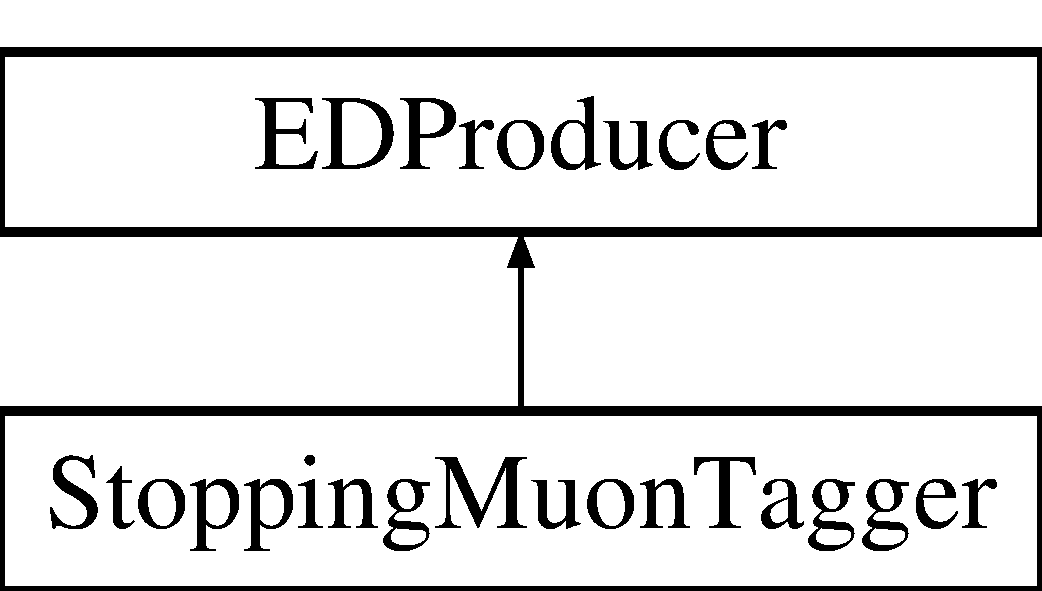
\includegraphics[height=2.000000cm]{classStoppingMuonTagger}
\end{center}
\end{figure}
\subsection*{Public Member Functions}
\begin{DoxyCompactItemize}
\item 
\hypertarget{classStoppingMuonTagger_a3ebd20018e8b0899e94bb3a01cc718be}{{\bfseries Stopping\-Muon\-Tagger} (fhicl\-::\-Parameter\-Set const \&p)}\label{classStoppingMuonTagger_a3ebd20018e8b0899e94bb3a01cc718be}

\item 
\hypertarget{classStoppingMuonTagger_a6a544fa555882979e4e288c91a362d75}{{\bfseries Stopping\-Muon\-Tagger} (\hyperlink{classStoppingMuonTagger}{Stopping\-Muon\-Tagger} const \&)=delete}\label{classStoppingMuonTagger_a6a544fa555882979e4e288c91a362d75}

\item 
\hypertarget{classStoppingMuonTagger_a9b6df4c680a52bfcc04a6c870d8b02c1}{{\bfseries Stopping\-Muon\-Tagger} (\hyperlink{classStoppingMuonTagger}{Stopping\-Muon\-Tagger} \&\&)=delete}\label{classStoppingMuonTagger_a9b6df4c680a52bfcc04a6c870d8b02c1}

\item 
\hypertarget{classStoppingMuonTagger_aa694be13fa360184be18359f555e788e}{\hyperlink{classStoppingMuonTagger}{Stopping\-Muon\-Tagger} \& {\bfseries operator=} (\hyperlink{classStoppingMuonTagger}{Stopping\-Muon\-Tagger} const \&)=delete}\label{classStoppingMuonTagger_aa694be13fa360184be18359f555e788e}

\item 
\hypertarget{classStoppingMuonTagger_a79fe9dd28e135cca483643a3b158656a}{\hyperlink{classStoppingMuonTagger}{Stopping\-Muon\-Tagger} \& {\bfseries operator=} (\hyperlink{classStoppingMuonTagger}{Stopping\-Muon\-Tagger} \&\&)=delete}\label{classStoppingMuonTagger_a79fe9dd28e135cca483643a3b158656a}

\item 
\hypertarget{classStoppingMuonTagger_acc39137db682cee3fac909296244b77a}{void {\bfseries produce} (art\-::\-Event \&e) override}\label{classStoppingMuonTagger_acc39137db682cee3fac909296244b77a}

\end{DoxyCompactItemize}


\subsection{Detailed Description}
Art producer module that tags stopping muons. 

\begin{DoxyAuthor}{Author}
Marco Del Tutto \href{mailto:marco.deltutto@physics.ox.ac.uk}{\tt marco.\-deltutto@physics.\-ox.\-ac.\-uk}
\end{DoxyAuthor}
\begin{DoxyVersion}{Version}
producer (art v2\-\_\-05\-\_\-00)
\end{DoxyVersion}
\begin{DoxyDate}{Date}
2017/03/10
\end{DoxyDate}
Contact\-: \href{mailto:marco.deltutto@physics.ox.ac.uk}{\tt marco.\-deltutto@physics.\-ox.\-ac.\-uk}

Created on\-: Fri Oct 6 15\-:55\-:20 2017 

The documentation for this class was generated from the following file\-:\begin{DoxyCompactItemize}
\item 
/home/travis/build/marcodeltutto/\-U\-B\-X\-Sec/\-Modules/Stopping\-Muon\-Tagger\-\_\-module.\-cc\end{DoxyCompactItemize}

\hypertarget{classubana_1_1TPCObject}{\section{ubana\-:\-:T\-P\-C\-Object Class Reference}
\label{classubana_1_1TPCObject}\index{ubana\-::\-T\-P\-C\-Object@{ubana\-::\-T\-P\-C\-Object}}
}


Data product to store a T\-P\-C Object.  




{\ttfamily \#include $<$T\-P\-C\-Object.\-h$>$}

\subsection*{Public Member Functions}
\begin{DoxyCompactItemize}
\item 
\hypertarget{classubana_1_1TPCObject_a0766c8648ada3d539b474e40a107d8c1}{void {\bfseries Set\-Tracks} (std\-::vector$<$ recob\-::\-Track $>$)}\label{classubana_1_1TPCObject_a0766c8648ada3d539b474e40a107d8c1}

\item 
\hypertarget{classubana_1_1TPCObject_a1fed8d9f87fc301a8cbee484a8434a05}{void {\bfseries Set\-Vertex} (recob\-::\-Vertex)}\label{classubana_1_1TPCObject_a1fed8d9f87fc301a8cbee484a8434a05}

\item 
\hypertarget{classubana_1_1TPCObject_ad4946cb455555486b701dd1301a26f56}{void {\bfseries Set\-Origin} (ubana\-::\-T\-P\-C\-Object\-Origin)}\label{classubana_1_1TPCObject_ad4946cb455555486b701dd1301a26f56}

\item 
\hypertarget{classubana_1_1TPCObject_a44cc29b00093d89d9f7fe834570d77be}{const std\-::vector$<$ recob\-::\-Track $>$ \& {\bfseries Get\-Tracks} () const }\label{classubana_1_1TPCObject_a44cc29b00093d89d9f7fe834570d77be}

\item 
\hypertarget{classubana_1_1TPCObject_a3845ae1b31ab6590c5597d157dc01e6a}{const recob\-::\-Vertex \& {\bfseries Get\-Vertex} () const }\label{classubana_1_1TPCObject_a3845ae1b31ab6590c5597d157dc01e6a}

\item 
\hypertarget{classubana_1_1TPCObject_a253b4e844b4de1333fa80263c03fceb7}{const ubana\-::\-T\-P\-C\-Object\-Origin \& {\bfseries Get\-Origin} () const }\label{classubana_1_1TPCObject_a253b4e844b4de1333fa80263c03fceb7}

\end{DoxyCompactItemize}


\subsection{Detailed Description}
Data product to store a T\-P\-C Object. 

\begin{DoxyAuthor}{Author}

\end{DoxyAuthor}
\begin{DoxyParagraph}{Author\-:}
Marco Del Tutto\href{mailto:marco.deltutto@physics.ox.ac.uk}{\tt marco.\-deltutto@physics.\-ox.\-ac.\-uk} 
\end{DoxyParagraph}


\begin{DoxyVersion}{Version}

\end{DoxyVersion}
\begin{DoxyParagraph}{Revision\-:}
1.\-0 
\end{DoxyParagraph}


\begin{DoxyDate}{Date}

\end{DoxyDate}
\begin{DoxyParagraph}{Date\-:}
2017/03/02 
\end{DoxyParagraph}


Contact\-: \href{mailto:marco.deltutto@physics.ox.ac.uk}{\tt marco.\-deltutto@physics.\-ox.\-ac.\-uk}

Created on\-: Friday, May 15, 2017 at 16\-:34\-:34 

The documentation for this class was generated from the following files\-:\begin{DoxyCompactItemize}
\item 
/home/travis/build/marcodeltutto/\-U\-B\-X\-Sec/\-Data\-Types/T\-P\-C\-Object.\-h\item 
/home/travis/build/marcodeltutto/\-U\-B\-X\-Sec/\-Data\-Types/T\-P\-C\-Object.\-cxx\end{DoxyCompactItemize}

\hypertarget{classubana_1_1TPCObjectFilter}{\section{ubana\-:\-:T\-P\-C\-Object\-Filter Class Reference}
\label{classubana_1_1TPCObjectFilter}\index{ubana\-::\-T\-P\-C\-Object\-Filter@{ubana\-::\-T\-P\-C\-Object\-Filter}}
}


{\ttfamily \#include $<$T\-P\-C\-Object\-Filter.\-h$>$}

\subsection*{Public Member Functions}
\begin{DoxyCompactItemize}
\item 
\hypertarget{classubana_1_1TPCObjectFilter_aa898a1ea96ce8bf1bf164111157a497d}{\hyperlink{classubana_1_1TPCObjectFilter_aa898a1ea96ce8bf1bf164111157a497d}{T\-P\-C\-Object\-Filter} ()}\label{classubana_1_1TPCObjectFilter_aa898a1ea96ce8bf1bf164111157a497d}

\begin{DoxyCompactList}\small\item\em Default constructor. \end{DoxyCompactList}\item 
\hypertarget{classubana_1_1TPCObjectFilter_ad8a3f726f247b5651272397ee344ef1e}{\hyperlink{classubana_1_1TPCObjectFilter_ad8a3f726f247b5651272397ee344ef1e}{$\sim$\-T\-P\-C\-Object\-Filter} ()}\label{classubana_1_1TPCObjectFilter_ad8a3f726f247b5651272397ee344ef1e}

\begin{DoxyCompactList}\small\item\em Default destructor. \end{DoxyCompactList}\item 
\hypertarget{classubana_1_1TPCObjectFilter_a49a5f29b105c442cc8fe97d05066c72a}{void \hyperlink{classubana_1_1TPCObjectFilter_a49a5f29b105c442cc8fe97d05066c72a}{Configure} (fhicl\-::\-Parameter\-Set const \&p)}\label{classubana_1_1TPCObjectFilter_a49a5f29b105c442cc8fe97d05066c72a}

\begin{DoxyCompactList}\small\item\em Configure function parameters. \end{DoxyCompactList}\item 
\hypertarget{classubana_1_1TPCObjectFilter_a542681a3872f6662e58e83330dddfe8c}{void \hyperlink{classubana_1_1TPCObjectFilter_a542681a3872f6662e58e83330dddfe8c}{Print\-Config} ()}\label{classubana_1_1TPCObjectFilter_a542681a3872f6662e58e83330dddfe8c}

\begin{DoxyCompactList}\small\item\em Printd the current configuration. \end{DoxyCompactList}\item 
\hypertarget{classubana_1_1TPCObjectFilter_ab485fca5770b8a9622d56c294b361ef3}{lar\-\_\-pandora\-::\-P\-F\-Particle\-Vector \hyperlink{classubana_1_1TPCObjectFilter_ab485fca5770b8a9622d56c294b361ef3}{Filter} (lar\-\_\-pandora\-::\-P\-F\-Particle\-Vector pfp\-\_\-v, lar\-\_\-pandora\-::\-P\-F\-Particles\-To\-Tracks pfp\-\_\-to\-\_\-tracks, lar\-\_\-pandora\-::\-P\-F\-Particles\-To\-Showers pfp\-\_\-to\-\_\-showers, lar\-\_\-pandora\-::\-P\-F\-Particles\-To\-Vertices pfp\-\_\-to\-\_\-vertices)}\label{classubana_1_1TPCObjectFilter_ab485fca5770b8a9622d56c294b361ef3}

\begin{DoxyCompactList}\small\item\em Returns a filtered vector of P\-F\-Particles\-: the new \hyperlink{classubana_1_1TPCObject}{T\-P\-C\-Object}. \end{DoxyCompactList}\end{DoxyCompactItemize}
\subsection*{Protected Attributes}
\begin{DoxyCompactItemize}
\item 
\hypertarget{classubana_1_1TPCObjectFilter_a86137c0a525fdd2b5a63afe4ff79c23c}{double \hyperlink{classubana_1_1TPCObjectFilter_a86137c0a525fdd2b5a63afe4ff79c23c}{\-\_\-tolerance}}\label{classubana_1_1TPCObjectFilter_a86137c0a525fdd2b5a63afe4ff79c23c}

\begin{DoxyCompactList}\small\item\em Tolerance for reclustering. \end{DoxyCompactList}\item 
\hypertarget{classubana_1_1TPCObjectFilter_a44156494ed6ccc98d9016c2c4306f282}{bool \hyperlink{classubana_1_1TPCObjectFilter_a44156494ed6ccc98d9016c2c4306f282}{\-\_\-debug}}\label{classubana_1_1TPCObjectFilter_a44156494ed6ccc98d9016c2c4306f282}

\begin{DoxyCompactList}\small\item\em Enabels debug printouts. \end{DoxyCompactList}\end{DoxyCompactItemize}


\subsection{Detailed Description}
User defined class \hyperlink{classubana_1_1TPCObjectFilter}{T\-P\-C\-Object\-Filter} ... these comments are used to generate doxygen documentation! 

The documentation for this class was generated from the following files\-:\begin{DoxyCompactItemize}
\item 
/home/travis/build/marcodeltutto/\-U\-B\-X\-Sec/\-Algorithms/\hyperlink{TPCObjectFilter_8h}{T\-P\-C\-Object\-Filter.\-h}\item 
/home/travis/build/marcodeltutto/\-U\-B\-X\-Sec/\-Algorithms/T\-P\-C\-Object\-Filter.\-cxx\end{DoxyCompactItemize}

\hypertarget{classubana_1_1TPCObjectMaker}{\section{ubana\-:\-:\-T\-P\-C\-Object\-Maker \-Class \-Reference}
\label{classubana_1_1TPCObjectMaker}\index{ubana\-::\-T\-P\-C\-Object\-Maker@{ubana\-::\-T\-P\-C\-Object\-Maker}}
}
\subsection*{\-Public \-Member \-Functions}
\begin{DoxyCompactItemize}
\item 
\hypertarget{group__UBXSec_gae030804e6aa4085bef6be52e9618fee9}{{\bfseries \-T\-P\-C\-Object\-Maker} (fhicl\-::\-Parameter\-Set const \&p)}\label{group__UBXSec_gae030804e6aa4085bef6be52e9618fee9}

\item 
\hypertarget{classubana_1_1TPCObjectMaker_a80b650974869e7c488654573955c7d9f}{{\bfseries \-T\-P\-C\-Object\-Maker} (\hyperlink{classubana_1_1TPCObjectMaker}{\-T\-P\-C\-Object\-Maker} const \&)}\label{classubana_1_1TPCObjectMaker_a80b650974869e7c488654573955c7d9f}

\item 
\hypertarget{classubana_1_1TPCObjectMaker_a94412d90dd82b0c1974ce2d5ff746aec}{{\bfseries \-T\-P\-C\-Object\-Maker} (\hyperlink{classubana_1_1TPCObjectMaker}{\-T\-P\-C\-Object\-Maker} \&\&)}\label{classubana_1_1TPCObjectMaker_a94412d90dd82b0c1974ce2d5ff746aec}

\item 
\hypertarget{classubana_1_1TPCObjectMaker_af87f91bc15450c410f21b2fef5c87c7b}{\hyperlink{classubana_1_1TPCObjectMaker}{\-T\-P\-C\-Object\-Maker} \& {\bfseries operator=} (\hyperlink{classubana_1_1TPCObjectMaker}{\-T\-P\-C\-Object\-Maker} const \&)}\label{classubana_1_1TPCObjectMaker_af87f91bc15450c410f21b2fef5c87c7b}

\item 
\hypertarget{classubana_1_1TPCObjectMaker_a949a6f5fe1f6ee0519ad0e550aa47dc8}{\hyperlink{classubana_1_1TPCObjectMaker}{\-T\-P\-C\-Object\-Maker} \& {\bfseries operator=} (\hyperlink{classubana_1_1TPCObjectMaker}{\-T\-P\-C\-Object\-Maker} \&\&)}\label{classubana_1_1TPCObjectMaker_a949a6f5fe1f6ee0519ad0e550aa47dc8}

\item 
\hypertarget{group__UBXSec_ga07c03a811bbaccdbeb20b2b7714034c9}{void {\bfseries produce} (art\-::\-Event \&e) override}\label{group__UBXSec_ga07c03a811bbaccdbeb20b2b7714034c9}

\item 
void \hyperlink{group__UBXSec_ga39991fa551ce05bcb4fb10db4f80ab49}{\-Collect\-Tracks\-And\-P\-F\-P} (lar\-\_\-pandora\-::\-P\-F\-Particles\-To\-Tracks pf\-Particle\-To\-Track\-Map, lar\-\_\-pandora\-::\-P\-F\-Particle\-Vector pf\-Particle\-List, art\-::\-Ptr$<$ recob\-::\-P\-F\-Particle $>$ particle, lar\-\_\-pandora\-::\-P\-F\-Particle\-Vector \&pfp\-\_\-v, lar\-\_\-pandora\-::\-Track\-Vector \&track\-\_\-v)
\begin{DoxyCompactList}\small\item\em \-Gets all the tracks and \-P\-F\-P for a single \-Pandora slice. \end{DoxyCompactList}\item 
void \hyperlink{group__UBXSec_gaf90fb2bf60601767e1db3bd1ca635433}{\-Get\-T\-P\-C\-Objects} (lar\-\_\-pandora\-::\-P\-F\-Particle\-Vector pf\-Particle\-List, lar\-\_\-pandora\-::\-P\-F\-Particles\-To\-Tracks pf\-Particle\-To\-Track\-Map, lar\-\_\-pandora\-::\-P\-F\-Particles\-To\-Vertices pf\-Particle\-To\-Vertex\-Map, std\-::vector$<$ lar\-\_\-pandora\-::\-P\-F\-Particle\-Vector $>$ \&pfp\-\_\-v\-\_\-v, std\-::vector$<$ lar\-\_\-pandora\-::\-Track\-Vector $>$ \&track\-\_\-v\-\_\-v)
\begin{DoxyCompactList}\small\item\em \-Constructs \-T\-P\-C objects using \-Pandora \-P\-F\-P slices. \end{DoxyCompactList}\item 
art\-::\-Ptr$<$ recob\-::\-P\-F\-Particle $>$ \hyperlink{group__UBXSec_ga6a47470b5f5690a3626e14bc9f6f360c}{\-Get\-Nu\-P\-F\-P} (lar\-\_\-pandora\-::\-P\-F\-Particle\-Vector pfp\-\_\-v)
\begin{DoxyCompactList}\small\item\em \-Returns the nu \-P\-F\-P from a \-T\-P\-C object. \end{DoxyCompactList}\end{DoxyCompactItemize}


\-The documentation for this class was generated from the following file\-:\begin{DoxyCompactItemize}
\item 
/home/travis/build/marcodeltutto/\-U\-B\-X\-Sec/\-Modules/\hyperlink{TPCObjectMaker__module_8cc}{\-T\-P\-C\-Object\-Maker\-\_\-module.\-cc}\end{DoxyCompactItemize}

\hypertarget{structubana_1_1two__points}{\section{ubana\-:\-:two\-\_\-points \-Struct \-Reference}
\label{structubana_1_1two__points}\index{ubana\-::two\-\_\-points@{ubana\-::two\-\_\-points}}
}
\subsection*{\-Public \-Attributes}
\begin{DoxyCompactItemize}
\item 
\hypertarget{structubana_1_1two__points_a7b4a3fb2486d98f65c2d1cc0e25ca20a}{\-T\-Vector3 {\bfseries pt1}}\label{structubana_1_1two__points_a7b4a3fb2486d98f65c2d1cc0e25ca20a}

\item 
\hypertarget{structubana_1_1two__points_ac013f258d66c091f55489a60ada46644}{\-T\-Vector3 {\bfseries pt2}}\label{structubana_1_1two__points_ac013f258d66c091f55489a60ada46644}

\item 
\hypertarget{structubana_1_1two__points_a50a483a90b03dc2e75ae4b187497047f}{bool {\bfseries good}}\label{structubana_1_1two__points_a50a483a90b03dc2e75ae4b187497047f}

\item 
\hypertarget{structubana_1_1two__points_a362517d5a9d32842eed0533e9a6c14bc}{bool {\bfseries is\-\_\-nu}}\label{structubana_1_1two__points_a362517d5a9d32842eed0533e9a6c14bc}

\end{DoxyCompactItemize}


\-The documentation for this struct was generated from the following file\-:\begin{DoxyCompactItemize}
\item 
/home/travis/build/marcodeltutto/\-U\-B\-X\-Sec/\-Algorithms/\-T\-P\-C\-Object\-Filter.\-cxx\end{DoxyCompactItemize}

\hypertarget{classUBXSec}{\section{\-U\-B\-X\-Sec \-Class \-Reference}
\label{classUBXSec}\index{\-U\-B\-X\-Sec@{\-U\-B\-X\-Sec}}
}


\-Art analyzer module.  


\subsection*{\-Public \-Member \-Functions}
\begin{DoxyCompactItemize}
\item 
\hypertarget{classUBXSec_a002d19d94378dc90587c10bd4b498c4b}{{\bfseries \-U\-B\-X\-Sec} (fhicl\-::\-Parameter\-Set const \&p)}\label{classUBXSec_a002d19d94378dc90587c10bd4b498c4b}

\item 
\hypertarget{classUBXSec_addfe39c7f3bf37d69254df5e87a9508b}{{\bfseries \-U\-B\-X\-Sec} (\hyperlink{classUBXSec}{\-U\-B\-X\-Sec} const \&)}\label{classUBXSec_addfe39c7f3bf37d69254df5e87a9508b}

\item 
\hypertarget{classUBXSec_a82ac81ae3bb5afe3f414449ad1cfa7ce}{{\bfseries \-U\-B\-X\-Sec} (\hyperlink{classUBXSec}{\-U\-B\-X\-Sec} \&\&)}\label{classUBXSec_a82ac81ae3bb5afe3f414449ad1cfa7ce}

\item 
\hypertarget{classUBXSec_a2fd957f5a0697d933bd55bfbc17fee46}{\hyperlink{classUBXSec}{\-U\-B\-X\-Sec} \& {\bfseries operator=} (\hyperlink{classUBXSec}{\-U\-B\-X\-Sec} const \&)}\label{classUBXSec_a2fd957f5a0697d933bd55bfbc17fee46}

\item 
\hypertarget{classUBXSec_a1034e664c80f3fbd3eea29d209f58196}{\hyperlink{classUBXSec}{\-U\-B\-X\-Sec} \& {\bfseries operator=} (\hyperlink{classUBXSec}{\-U\-B\-X\-Sec} \&\&)}\label{classUBXSec_a1034e664c80f3fbd3eea29d209f58196}

\item 
\hypertarget{classUBXSec_a30a2981a63a32be7d7b8819bb462e859}{void {\bfseries analyze} (art\-::\-Event const \&e) override}\label{classUBXSec_a30a2981a63a32be7d7b8819bb462e859}

\end{DoxyCompactItemize}


\subsection{\-Detailed \-Description}
\-Art analyzer module. 

\begin{DoxyAuthor}{\-Author}

\end{DoxyAuthor}
\begin{DoxyParagraph}{\-Author\-:}
\-Marco \-Del \-Tutto$<$\href{mailto:marco.deltutto@physics.ox.ac.uk}{\tt marco.\-deltutto@physics.\-ox.\-ac.\-uk}$>$ 
\end{DoxyParagraph}


\begin{DoxyVersion}{\-Version}

\end{DoxyVersion}
\begin{DoxyParagraph}{\-Revision\-:}
1.\-0 
\end{DoxyParagraph}


\begin{DoxyDate}{\-Date}

\end{DoxyDate}
\begin{DoxyParagraph}{\-Date\-:}
2017/03/10 
\end{DoxyParagraph}


\-Contact\-: \href{mailto:marco.deltutto@physics.ox.ac.uk}{\tt marco.\-deltutto@physics.\-ox.\-ac.\-uk}

\-Created on\-: \-Friday, \-March 10, 2017 at 12\-:32\-:31 

\-The documentation for this class was generated from the following file\-:\begin{DoxyCompactItemize}
\item 
/home/travis/build/marcodeltutto/\-U\-B\-X\-Sec/\-Modules/\-U\-B\-X\-Sec\-\_\-module.\-cc\end{DoxyCompactItemize}

\hypertarget{classUBXSecEvent}{\section{U\-B\-X\-Sec\-Event Class Reference}
\label{classUBXSecEvent}\index{U\-B\-X\-Sec\-Event@{U\-B\-X\-Sec\-Event}}
}


Data product to store a \hyperlink{classUBXSec}{U\-B\-X\-Sec} Event.  




{\ttfamily \#include $<$U\-B\-X\-Sec\-Event.\-h$>$}

\subsection*{Public Member Functions}
\begin{DoxyCompactItemize}
\item 
\hypertarget{classUBXSecEvent_a57603c847176b408838d04e690b04828}{void {\bfseries Init} ()}\label{classUBXSecEvent_a57603c847176b408838d04e690b04828}

\item 
\hypertarget{classUBXSecEvent_a87228eb442b415053b9a9a070d29790b}{void {\bfseries Resize\-Vectors} (int)}\label{classUBXSecEvent_a87228eb442b415053b9a9a070d29790b}

\end{DoxyCompactItemize}
\subsection*{Public Attributes}
\begin{DoxyCompactItemize}
\item 
\hypertarget{classUBXSecEvent_ad26e1c100cfe11d9f7c48a3760cdcc07}{Int\-\_\-t \hyperlink{classUBXSecEvent_ad26e1c100cfe11d9f7c48a3760cdcc07}{run}}\label{classUBXSecEvent_ad26e1c100cfe11d9f7c48a3760cdcc07}

\begin{DoxyCompactList}\small\item\em Run number. \end{DoxyCompactList}\item 
\hypertarget{classUBXSecEvent_a15ac0be3ec941ed67ee78d27da704abb}{Int\-\_\-t \hyperlink{classUBXSecEvent_a15ac0be3ec941ed67ee78d27da704abb}{subrun}}\label{classUBXSecEvent_a15ac0be3ec941ed67ee78d27da704abb}

\begin{DoxyCompactList}\small\item\em Subrun number. \end{DoxyCompactList}\item 
\hypertarget{classUBXSecEvent_a5833c043eb96d5d41935cd1c6eaec722}{Int\-\_\-t \hyperlink{classUBXSecEvent_a5833c043eb96d5d41935cd1c6eaec722}{event}}\label{classUBXSecEvent_a5833c043eb96d5d41935cd1c6eaec722}

\begin{DoxyCompactList}\small\item\em Event number. \end{DoxyCompactList}\item 
\hypertarget{classUBXSecEvent_a429e2c8750cdd32b073548b73c5ebd68}{Bool\-\_\-t \hyperlink{classUBXSecEvent_a429e2c8750cdd32b073548b73c5ebd68}{muon\-\_\-is\-\_\-reco}}\label{classUBXSecEvent_a429e2c8750cdd32b073548b73c5ebd68}

\begin{DoxyCompactList}\small\item\em Is true if the muon from the neutrino interaction is reconstructed. \end{DoxyCompactList}\item 
\hypertarget{classUBXSecEvent_ac1391d470b732d86bb9e462d49fff185}{Double\-\_\-t \hyperlink{classUBXSecEvent_ac1391d470b732d86bb9e462d49fff185}{muon\-\_\-reco\-\_\-pur}}\label{classUBXSecEvent_ac1391d470b732d86bb9e462d49fff185}

\begin{DoxyCompactList}\small\item\em If reco, stores the reco muon purity. \end{DoxyCompactList}\item 
\hypertarget{classUBXSecEvent_aa713bc31919706a03a5a11034dcbda7c}{Double\-\_\-t \hyperlink{classUBXSecEvent_aa713bc31919706a03a5a11034dcbda7c}{muon\-\_\-reco\-\_\-eff}}\label{classUBXSecEvent_aa713bc31919706a03a5a11034dcbda7c}

\begin{DoxyCompactList}\small\item\em If reco, stores the reco muon efficiency. \end{DoxyCompactList}\item 
\hypertarget{classUBXSecEvent_a967af89c3282493ba4ec96a4bf1592e9}{Double\-\_\-t \hyperlink{classUBXSecEvent_a967af89c3282493ba4ec96a4bf1592e9}{true\-\_\-muon\-\_\-mom}}\label{classUBXSecEvent_a967af89c3282493ba4ec96a4bf1592e9}

\begin{DoxyCompactList}\small\item\em If exists, stores the true muon momentum. \end{DoxyCompactList}\item 
\hypertarget{classUBXSecEvent_ac01db50f50e39aed219935666f441aed}{Double\-\_\-t \hyperlink{classUBXSecEvent_ac01db50f50e39aed219935666f441aed}{true\-\_\-muon\-\_\-mom\-\_\-matched}}\label{classUBXSecEvent_ac01db50f50e39aed219935666f441aed}

\begin{DoxyCompactList}\small\item\em True momentum of the M\-C\-P matched to the muon P\-F\-P. \end{DoxyCompactList}\item 
\hypertarget{classUBXSecEvent_a966e90da255666b555c301b83385e923}{Int\-\_\-t \hyperlink{classUBXSecEvent_a966e90da255666b555c301b83385e923}{n\-\_\-pfp}}\label{classUBXSecEvent_a966e90da255666b555c301b83385e923}

\begin{DoxyCompactList}\small\item\em Number of P\-F\-P in the event. \end{DoxyCompactList}\item 
\hypertarget{classUBXSecEvent_a8b42a4c5da11c709d44d6f51933d7687}{Int\-\_\-t \hyperlink{classUBXSecEvent_a8b42a4c5da11c709d44d6f51933d7687}{n\-\_\-pfp\-\_\-primary}}\label{classUBXSecEvent_a8b42a4c5da11c709d44d6f51933d7687}

\begin{DoxyCompactList}\small\item\em Number of primary P\-F\-P in the event (neutrino P\-F\-P) \end{DoxyCompactList}\item 
\hypertarget{classUBXSecEvent_ae57001de3cd8374785329521c3ce5d5e}{Int\-\_\-t \hyperlink{classUBXSecEvent_ae57001de3cd8374785329521c3ce5d5e}{n\-\_\-primary\-\_\-cosmic\-\_\-pfp}}\label{classUBXSecEvent_ae57001de3cd8374785329521c3ce5d5e}

\begin{DoxyCompactList}\small\item\em Number of primary P\-F\-P in the event from pandora\-Cosmic (primaries before the removal) \end{DoxyCompactList}\item 
\hypertarget{classUBXSecEvent_a64e18b32773515202fcb167d1818133b}{Int\-\_\-t \hyperlink{classUBXSecEvent_a64e18b32773515202fcb167d1818133b}{n\-P\-F\-Ptagged}}\label{classUBXSecEvent_a64e18b32773515202fcb167d1818133b}

\begin{DoxyCompactList}\small\item\em Not used. \end{DoxyCompactList}\item 
\hypertarget{classUBXSecEvent_a33857278922a2779d3daaf30624a2462}{Int\-\_\-t \hyperlink{classUBXSecEvent_a33857278922a2779d3daaf30624a2462}{muon\-\_\-is\-\_\-flash\-\_\-tagged}}\label{classUBXSecEvent_a33857278922a2779d3daaf30624a2462}

\begin{DoxyCompactList}\small\item\em Not used. \end{DoxyCompactList}\item 
\hypertarget{classUBXSecEvent_a492e788ae84c0ac6c847b7ba95656706}{Double\-\_\-t \hyperlink{classUBXSecEvent_a492e788ae84c0ac6c847b7ba95656706}{muon\-\_\-tag\-\_\-score}}\label{classUBXSecEvent_a492e788ae84c0ac6c847b7ba95656706}

\begin{DoxyCompactList}\small\item\em Not used. \end{DoxyCompactList}\item 
\hypertarget{classUBXSecEvent_af45f0efa722a046884ec4f6c36b77d9a}{Double\-\_\-t \hyperlink{classUBXSecEvent_af45f0efa722a046884ec4f6c36b77d9a}{fm\-\_\-score}}\label{classUBXSecEvent_af45f0efa722a046884ec4f6c36b77d9a}

\begin{DoxyCompactList}\small\item\em Not used. \end{DoxyCompactList}\item 
\hypertarget{classUBXSecEvent_a3b05f41e3b302767d921996aed6f0d87}{Int\-\_\-t \hyperlink{classUBXSecEvent_a3b05f41e3b302767d921996aed6f0d87}{fv}}\label{classUBXSecEvent_a3b05f41e3b302767d921996aed6f0d87}

\begin{DoxyCompactList}\small\item\em Is 1 if the true neutrino vertex is in the fiducial volume. \end{DoxyCompactList}\item 
\hypertarget{classUBXSecEvent_a6a55ef25451d4a8206055d588b052caf}{Int\-\_\-t \hyperlink{classUBXSecEvent_a6a55ef25451d4a8206055d588b052caf}{ccnc}}\label{classUBXSecEvent_a6a55ef25451d4a8206055d588b052caf}

\begin{DoxyCompactList}\small\item\em Is 0 if C\-C, 1 if N\-C. \end{DoxyCompactList}\item 
\hypertarget{classUBXSecEvent_a61f5c298a7cebb0c5286b4ed4c7a0627}{Int\-\_\-t \hyperlink{classUBXSecEvent_a61f5c298a7cebb0c5286b4ed4c7a0627}{nupdg}}\label{classUBXSecEvent_a61f5c298a7cebb0c5286b4ed4c7a0627}

\begin{DoxyCompactList}\small\item\em Neutrino flavour (pdg code) \end{DoxyCompactList}\item 
\hypertarget{classUBXSecEvent_a2cc7d9f302e0d413ece8af96b35fcff0}{Bool\-\_\-t \hyperlink{classUBXSecEvent_a2cc7d9f302e0d413ece8af96b35fcff0}{is\-\_\-signal}}\label{classUBXSecEvent_a2cc7d9f302e0d413ece8af96b35fcff0}

\begin{DoxyCompactList}\small\item\em Is trues if the event is a true numu cc in F\-V. \end{DoxyCompactList}\item 
\hypertarget{classUBXSecEvent_a715a5f6d8143a633109ed48fb87e0bbd}{Double\-\_\-t \hyperlink{classUBXSecEvent_a715a5f6d8143a633109ed48fb87e0bbd}{nu\-\_\-e}}\label{classUBXSecEvent_a715a5f6d8143a633109ed48fb87e0bbd}

\begin{DoxyCompactList}\small\item\em Stores the true neutrino energy. \end{DoxyCompactList}\item 
\hypertarget{classUBXSecEvent_a57ac9edd2e200ea54da22ee278079857}{Double\-\_\-t \hyperlink{classUBXSecEvent_a57ac9edd2e200ea54da22ee278079857}{lep\-\_\-costheta}}\label{classUBXSecEvent_a57ac9edd2e200ea54da22ee278079857}

\begin{DoxyCompactList}\small\item\em Lepton true cos\-Thata angle at start. \end{DoxyCompactList}\item 
\hypertarget{classUBXSecEvent_a7b4229f9ab6a20424bffd9ef5a57edc6}{Double\-\_\-t \hyperlink{classUBXSecEvent_a7b4229f9ab6a20424bffd9ef5a57edc6}{lep\-\_\-phi}}\label{classUBXSecEvent_a7b4229f9ab6a20424bffd9ef5a57edc6}

\begin{DoxyCompactList}\small\item\em Lepton true Phi angle at start. \end{DoxyCompactList}\item 
\hypertarget{classUBXSecEvent_a767300e775e92348238668ef99dfdbc8}{Int\-\_\-t \hyperlink{classUBXSecEvent_a767300e775e92348238668ef99dfdbc8}{genie\-\_\-mult}}\label{classUBXSecEvent_a767300e775e92348238668ef99dfdbc8}

\begin{DoxyCompactList}\small\item\em Number of stable G\-E\-N\-I\-E final state particles. \end{DoxyCompactList}\item 
\hypertarget{classUBXSecEvent_a6a73137488dc2af0dc6abd5868fbbe4d}{Int\-\_\-t \hyperlink{classUBXSecEvent_a6a73137488dc2af0dc6abd5868fbbe4d}{genie\-\_\-mult\-\_\-ch}}\label{classUBXSecEvent_a6a73137488dc2af0dc6abd5868fbbe4d}

\begin{DoxyCompactList}\small\item\em Number of stable charged G\-E\-N\-I\-E final state particles. \end{DoxyCompactList}\item 
\hypertarget{classUBXSecEvent_a350303f94db8bcfdbc2e517713d7ebf9}{Int\-\_\-t \hyperlink{classUBXSecEvent_a350303f94db8bcfdbc2e517713d7ebf9}{mc\-\_\-muon\-\_\-contained}}\label{classUBXSecEvent_a350303f94db8bcfdbc2e517713d7ebf9}

\begin{DoxyCompactList}\small\item\em Is 1 if the true mc muon is fully contained. \end{DoxyCompactList}\item 
\hypertarget{classUBXSecEvent_aedee1ade9f68dfb32fba0b943125f52d}{Int\-\_\-t \hyperlink{classUBXSecEvent_aedee1ade9f68dfb32fba0b943125f52d}{is\-\_\-swtriggered}}\label{classUBXSecEvent_aedee1ade9f68dfb32fba0b943125f52d}

\begin{DoxyCompactList}\small\item\em Is true if the event passed the software trigger. \end{DoxyCompactList}\item 
\hypertarget{classUBXSecEvent_aa6c3a4dd22dfd2d39be8fa74b3703230}{Double\-\_\-t \hyperlink{classUBXSecEvent_aa6c3a4dd22dfd2d39be8fa74b3703230}{vtx\-\_\-resolution}}\label{classUBXSecEvent_aa6c3a4dd22dfd2d39be8fa74b3703230}

\begin{DoxyCompactList}\small\item\em Stores the vertex resolution. \end{DoxyCompactList}\item 
\hypertarget{classUBXSecEvent_a0ae9b16a767089e072f0b82da7e071d4}{Int\-\_\-t \hyperlink{classUBXSecEvent_a0ae9b16a767089e072f0b82da7e071d4}{n\-\_\-tpcobj\-\_\-nu\-\_\-origin}}\label{classUBXSecEvent_a0ae9b16a767089e072f0b82da7e071d4}

\begin{DoxyCompactList}\small\item\em Number of T\-P\-C\-Objects with neutrino origin in the event. \end{DoxyCompactList}\item 
\hypertarget{classUBXSecEvent_a64e81de34497d79043b873862c28fd87}{Int\-\_\-t \hyperlink{classUBXSecEvent_a64e81de34497d79043b873862c28fd87}{n\-\_\-tpcobj\-\_\-cosmic\-\_\-origin}}\label{classUBXSecEvent_a64e81de34497d79043b873862c28fd87}

\begin{DoxyCompactList}\small\item\em Number of T\-P\-C\-Objects with cosmic origin in the event. \end{DoxyCompactList}\item 
\hypertarget{classUBXSecEvent_abcf4435958fac040ad4e3c85802eea27}{Int\-\_\-t \hyperlink{classUBXSecEvent_abcf4435958fac040ad4e3c85802eea27}{nslices}}\label{classUBXSecEvent_abcf4435958fac040ad4e3c85802eea27}

\begin{DoxyCompactList}\small\item\em Stores the number of T\-P\-C\-Objects in the event. \end{DoxyCompactList}\item 
\hypertarget{classUBXSecEvent_aac7860c3885997956aabf560254afb42}{vector$<$ double $>$ \hyperlink{classUBXSecEvent_aac7860c3885997956aabf560254afb42}{slc\-\_\-flsmatch\-\_\-score}}\label{classUBXSecEvent_aac7860c3885997956aabf560254afb42}

\begin{DoxyCompactList}\small\item\em Flash matching score (-\/9999 means failed to match) \end{DoxyCompactList}\item 
\hypertarget{classUBXSecEvent_abc1d1ba9d1ce91ae8784f3e99deb6ebb}{vector$<$ double $>$ \hyperlink{classUBXSecEvent_abc1d1ba9d1ce91ae8784f3e99deb6ebb}{slc\-\_\-flsmatch\-\_\-qllx}}\label{classUBXSecEvent_abc1d1ba9d1ce91ae8784f3e99deb6ebb}

\begin{DoxyCompactList}\small\item\em Estimated X position given by flash matching. \end{DoxyCompactList}\item 
\hypertarget{classUBXSecEvent_afc096cb78a5130678717f9c513e6b90c}{vector$<$ double $>$ \hyperlink{classUBXSecEvent_afc096cb78a5130678717f9c513e6b90c}{slc\-\_\-flsmatch\-\_\-tpcx}}\label{classUBXSecEvent_afc096cb78a5130678717f9c513e6b90c}

\begin{DoxyCompactList}\small\item\em T\-P\-C X position given by the flash time. \end{DoxyCompactList}\item 
\hypertarget{classUBXSecEvent_af4f355424e0a80580b581268eb25dd12}{vector$<$ double $>$ \hyperlink{classUBXSecEvent_af4f355424e0a80580b581268eb25dd12}{slc\-\_\-flsmatch\-\_\-t0}}\label{classUBXSecEvent_af4f355424e0a80580b581268eb25dd12}

\begin{DoxyCompactList}\small\item\em Time of the beam spill flash. \end{DoxyCompactList}\item 
\hypertarget{classUBXSecEvent_a237e3f0d9a59f740ee1725fd7d8186bd}{vector$<$ double $>$ \hyperlink{classUBXSecEvent_a237e3f0d9a59f740ee1725fd7d8186bd}{slc\-\_\-flsmatch\-\_\-hypoz}}\label{classUBXSecEvent_a237e3f0d9a59f740ee1725fd7d8186bd}

\begin{DoxyCompactList}\small\item\em Z center of the hypothesis flash. \end{DoxyCompactList}\item 
\hypertarget{classUBXSecEvent_a51b8f4fca1456ceba66f171ac8e9eb4a}{vector$<$ double $>$ \hyperlink{classUBXSecEvent_a51b8f4fca1456ceba66f171ac8e9eb4a}{slc\-\_\-flsmatch\-\_\-xfixed\-\_\-chi2}}\label{classUBXSecEvent_a51b8f4fca1456ceba66f171ac8e9eb4a}

\begin{DoxyCompactList}\small\item\em Not used. \end{DoxyCompactList}\item 
\hypertarget{classUBXSecEvent_a1bf76c945234f61391ad4d287862f2a8}{vector$<$ double $>$ \hyperlink{classUBXSecEvent_a1bf76c945234f61391ad4d287862f2a8}{slc\-\_\-flsmatch\-\_\-xfixed\-\_\-ll}}\label{classUBXSecEvent_a1bf76c945234f61391ad4d287862f2a8}

\begin{DoxyCompactList}\small\item\em Not used. \end{DoxyCompactList}\item 
\hypertarget{classUBXSecEvent_ad74c03fcc0b57d4084eb05d0f5617b3a}{vector$<$ double $>$ \hyperlink{classUBXSecEvent_ad74c03fcc0b57d4084eb05d0f5617b3a}{slc\-\_\-flsmatch\-\_\-cosmic\-\_\-score}}\label{classUBXSecEvent_ad74c03fcc0b57d4084eb05d0f5617b3a}

\begin{DoxyCompactList}\small\item\em Not used. \end{DoxyCompactList}\item 
\hypertarget{classUBXSecEvent_a645973d4e447d46008828658b826e8f0}{vector$<$ double $>$ \hyperlink{classUBXSecEvent_a645973d4e447d46008828658b826e8f0}{slc\-\_\-flsmatch\-\_\-cosmic\-\_\-t0}}\label{classUBXSecEvent_a645973d4e447d46008828658b826e8f0}

\begin{DoxyCompactList}\small\item\em Not used. \end{DoxyCompactList}\item 
\hypertarget{classUBXSecEvent_ac97e86f7559ceb52bacb97bd60c25f09}{vector$<$ double $>$ \hyperlink{classUBXSecEvent_ac97e86f7559ceb52bacb97bd60c25f09}{slc\-\_\-nuvtx\-\_\-x}}\label{classUBXSecEvent_ac97e86f7559ceb52bacb97bd60c25f09}

\begin{DoxyCompactList}\small\item\em Reconstructed neutrino vertex X (cm) \end{DoxyCompactList}\item 
\hypertarget{classUBXSecEvent_aabba0cbb738793a9713deb8888d3919b}{vector$<$ double $>$ \hyperlink{classUBXSecEvent_aabba0cbb738793a9713deb8888d3919b}{slc\-\_\-nuvtx\-\_\-y}}\label{classUBXSecEvent_aabba0cbb738793a9713deb8888d3919b}

\begin{DoxyCompactList}\small\item\em Reconstructed neutrino vertex Y (cm) \end{DoxyCompactList}\item 
\hypertarget{classUBXSecEvent_abc7e1a40fd182e817c83e5e4066eeb07}{vector$<$ double $>$ \hyperlink{classUBXSecEvent_abc7e1a40fd182e817c83e5e4066eeb07}{slc\-\_\-nuvtx\-\_\-z}}\label{classUBXSecEvent_abc7e1a40fd182e817c83e5e4066eeb07}

\begin{DoxyCompactList}\small\item\em Reconstructed neutrino vertex Z (cm) \end{DoxyCompactList}\item 
\hypertarget{classUBXSecEvent_ae5160345d6d863bbe3ad2abb19298dc6}{vector$<$ int $>$ \hyperlink{classUBXSecEvent_ae5160345d6d863bbe3ad2abb19298dc6}{slc\-\_\-nuvtx\-\_\-fv}}\label{classUBXSecEvent_ae5160345d6d863bbe3ad2abb19298dc6}

\begin{DoxyCompactList}\small\item\em Is 1 if the recon neutrino vertex is in the fiducial volume. \end{DoxyCompactList}\item 
\hypertarget{classUBXSecEvent_af9855bb4f1c558d9032c3059beb49015}{vector$<$ double $>$ \hyperlink{classUBXSecEvent_af9855bb4f1c558d9032c3059beb49015}{slc\-\_\-vtxcheck\-\_\-angle}}\label{classUBXSecEvent_af9855bb4f1c558d9032c3059beb49015}

\begin{DoxyCompactList}\small\item\em Angle between longest tracks (if extist, -\/9999 otherwise) \end{DoxyCompactList}\item 
\hypertarget{classUBXSecEvent_aebb1b1e843015c57cd10b411682dbb2e}{vector$<$ int $>$ \hyperlink{classUBXSecEvent_aebb1b1e843015c57cd10b411682dbb2e}{slc\-\_\-origin}}\label{classUBXSecEvent_aebb1b1e843015c57cd10b411682dbb2e}

\begin{DoxyCompactList}\small\item\em Origin of the slice (0\-: neutrino, 1\-: cosmic, 2\-: mixed) (M\-C only) \end{DoxyCompactList}\item 
\hypertarget{classUBXSecEvent_ac1532ccdcb92b158c2393ec6a2a816f8}{vector$<$ int $>$ \hyperlink{classUBXSecEvent_ac1532ccdcb92b158c2393ec6a2a816f8}{slc\-\_\-origin\-\_\-extra}}\label{classUBXSecEvent_ac1532ccdcb92b158c2393ec6a2a816f8}

\begin{DoxyCompactList}\small\item\em Origin extra of the slice (-\/1\-: not set, 0\-: stopping muon, 1\-: acpt, 2\-: ncpion, 3\-: ncproton) (M\-C only) \end{DoxyCompactList}\item 
\hypertarget{classUBXSecEvent_a52bec741eadb5ef5f4bf1c2322707d20}{vector$<$ int $>$ \hyperlink{classUBXSecEvent_a52bec741eadb5ef5f4bf1c2322707d20}{slc\-\_\-nhits\-\_\-u}}\label{classUBXSecEvent_a52bec741eadb5ef5f4bf1c2322707d20}

\begin{DoxyCompactList}\small\item\em Number of hits on the U plane. \end{DoxyCompactList}\item 
\hypertarget{classUBXSecEvent_a5ade1b25620def646196c0d7fa3ad7f3}{vector$<$ int $>$ \hyperlink{classUBXSecEvent_a5ade1b25620def646196c0d7fa3ad7f3}{slc\-\_\-nhits\-\_\-v}}\label{classUBXSecEvent_a5ade1b25620def646196c0d7fa3ad7f3}

\begin{DoxyCompactList}\small\item\em Number of hits on the V plane. \end{DoxyCompactList}\item 
\hypertarget{classUBXSecEvent_ac20d2a610a09c19bb6c10e80ec735b12}{vector$<$ int $>$ \hyperlink{classUBXSecEvent_ac20d2a610a09c19bb6c10e80ec735b12}{slc\-\_\-nhits\-\_\-w}}\label{classUBXSecEvent_ac20d2a610a09c19bb6c10e80ec735b12}

\begin{DoxyCompactList}\small\item\em Number of hits on the W plane. \end{DoxyCompactList}\item 
\hypertarget{classUBXSecEvent_ac3a7dd3d816188675925b73049cddc2a}{vector$<$ double $>$ \hyperlink{classUBXSecEvent_ac3a7dd3d816188675925b73049cddc2a}{slc\-\_\-longesttrack\-\_\-length}}\label{classUBXSecEvent_ac3a7dd3d816188675925b73049cddc2a}

\begin{DoxyCompactList}\small\item\em Length of the longest track. \end{DoxyCompactList}\item 
\hypertarget{classUBXSecEvent_a3d3b0be1ba8321dfa3f19fad27ae654c}{vector$<$ double $>$ \hyperlink{classUBXSecEvent_a3d3b0be1ba8321dfa3f19fad27ae654c}{slc\-\_\-longesttrack\-\_\-phi}}\label{classUBXSecEvent_a3d3b0be1ba8321dfa3f19fad27ae654c}

\begin{DoxyCompactList}\small\item\em Phi angle of the longest track. \end{DoxyCompactList}\item 
\hypertarget{classUBXSecEvent_aa3f16db3a887ed53354cae2bb3de19cb}{vector$<$ double $>$ \hyperlink{classUBXSecEvent_aa3f16db3a887ed53354cae2bb3de19cb}{slc\-\_\-longesttrack\-\_\-theta}}\label{classUBXSecEvent_aa3f16db3a887ed53354cae2bb3de19cb}

\begin{DoxyCompactList}\small\item\em Cos(theta) of the longest track. \end{DoxyCompactList}\item 
\hypertarget{classUBXSecEvent_a2e715c70dcf023fddf77ef56c85d01cf}{vector$<$ bool $>$ \hyperlink{classUBXSecEvent_a2e715c70dcf023fddf77ef56c85d01cf}{slc\-\_\-longesttrack\-\_\-iscontained}}\label{classUBXSecEvent_a2e715c70dcf023fddf77ef56c85d01cf}

\begin{DoxyCompactList}\small\item\em Is true if the longest track if fully contained. \end{DoxyCompactList}\item 
\hypertarget{classUBXSecEvent_afd52675b8ca60af2941105f9739909a4}{vector$<$ int $>$ \hyperlink{classUBXSecEvent_afd52675b8ca60af2941105f9739909a4}{slc\-\_\-acpt\-\_\-outoftime}}\label{classUBXSecEvent_afd52675b8ca60af2941105f9739909a4}

\begin{DoxyCompactList}\small\item\em Not used. \end{DoxyCompactList}\item 
\hypertarget{classUBXSecEvent_ae7aee5c97b811d2e867cab5ec4fa1ffd}{vector$<$ int $>$ \hyperlink{classUBXSecEvent_ae7aee5c97b811d2e867cab5ec4fa1ffd}{slc\-\_\-crosses\-\_\-top\-\_\-boundary}}\label{classUBXSecEvent_ae7aee5c97b811d2e867cab5ec4fa1ffd}

\begin{DoxyCompactList}\small\item\em Is 1 if the track crosses the top roof of the T\-P\-C. \end{DoxyCompactList}\item 
\hypertarget{classUBXSecEvent_a702fda60b130a5de87b4cd5639b111d6}{vector$<$ int $>$ \hyperlink{classUBXSecEvent_a702fda60b130a5de87b4cd5639b111d6}{slc\-\_\-nuvtx\-\_\-closetodeadregion\-\_\-u}}\label{classUBXSecEvent_a702fda60b130a5de87b4cd5639b111d6}

\begin{DoxyCompactList}\small\item\em Is 1 if the recon nu vertex is close to a dead region on the U plane. \end{DoxyCompactList}\item 
\hypertarget{classUBXSecEvent_aea1570a2a53f22dcbbe2d0c349502a3b}{vector$<$ int $>$ \hyperlink{classUBXSecEvent_aea1570a2a53f22dcbbe2d0c349502a3b}{slc\-\_\-nuvtx\-\_\-closetodeadregion\-\_\-v}}\label{classUBXSecEvent_aea1570a2a53f22dcbbe2d0c349502a3b}

\begin{DoxyCompactList}\small\item\em Is 1 if the recon nu vertex is close to a dead region on the V plane. \end{DoxyCompactList}\item 
\hypertarget{classUBXSecEvent_a0e32deb7f9e8d3f4356b52dfa74892ad}{vector$<$ int $>$ \hyperlink{classUBXSecEvent_a0e32deb7f9e8d3f4356b52dfa74892ad}{slc\-\_\-nuvtx\-\_\-closetodeadregion\-\_\-w}}\label{classUBXSecEvent_a0e32deb7f9e8d3f4356b52dfa74892ad}

\begin{DoxyCompactList}\small\item\em Is 1 if the recon nu vertex is close to a dead region on the W plane. \end{DoxyCompactList}\item 
\hypertarget{classUBXSecEvent_a7b3a38020a5ff375b9a9632c6eda9845}{vector$<$ double $>$ \hyperlink{classUBXSecEvent_a7b3a38020a5ff375b9a9632c6eda9845}{slc\-\_\-kalman\-\_\-chi2}}\label{classUBXSecEvent_a7b3a38020a5ff375b9a9632c6eda9845}

\begin{DoxyCompactList}\small\item\em Not used. \end{DoxyCompactList}\item 
\hypertarget{classUBXSecEvent_ac4a8b79e4a4b02254ede89b475f3ca5c}{vector$<$ int $>$ \hyperlink{classUBXSecEvent_ac4a8b79e4a4b02254ede89b475f3ca5c}{slc\-\_\-kalman\-\_\-ndof}}\label{classUBXSecEvent_ac4a8b79e4a4b02254ede89b475f3ca5c}

\begin{DoxyCompactList}\small\item\em Not used. \end{DoxyCompactList}\item 
\hypertarget{classUBXSecEvent_aab3be8887f062f848104113097b27ad5}{vector$<$ bool $>$ \hyperlink{classUBXSecEvent_aab3be8887f062f848104113097b27ad5}{slc\-\_\-passed\-\_\-min\-\_\-track\-\_\-quality}}\label{classUBXSecEvent_aab3be8887f062f848104113097b27ad5}

\begin{DoxyCompactList}\small\item\em Is true if the T\-P\-C\-Object passed track minimum quality requirements. \end{DoxyCompactList}\item 
\hypertarget{classUBXSecEvent_af2bdc55d1c56cea1c4e3104e262f029c}{vector$<$ bool $>$ \hyperlink{classUBXSecEvent_af2bdc55d1c56cea1c4e3104e262f029c}{slc\-\_\-passed\-\_\-min\-\_\-vertex\-\_\-quality}}\label{classUBXSecEvent_af2bdc55d1c56cea1c4e3104e262f029c}

\begin{DoxyCompactList}\small\item\em Is true if the T\-P\-C\-Object passed track minimum vertex requirements. \end{DoxyCompactList}\item 
\hypertarget{classUBXSecEvent_a8234ab4e219c1355370b5f141ad10211}{vector$<$ double $>$ \hyperlink{classUBXSecEvent_a8234ab4e219c1355370b5f141ad10211}{slc\-\_\-n\-\_\-intime\-\_\-pe\-\_\-closestpmt}}\label{classUBXSecEvent_a8234ab4e219c1355370b5f141ad10211}

\begin{DoxyCompactList}\small\item\em Not used. \end{DoxyCompactList}\item 
\hypertarget{classUBXSecEvent_afbcefec1936192c7a46b3414d7f3067d}{vector$<$ double $>$ \hyperlink{classUBXSecEvent_afbcefec1936192c7a46b3414d7f3067d}{slc\-\_\-maxdistance\-\_\-vtxtrack}}\label{classUBXSecEvent_afbcefec1936192c7a46b3414d7f3067d}

\begin{DoxyCompactList}\small\item\em Not used. \end{DoxyCompactList}\item 
\hypertarget{classUBXSecEvent_a5bf2adbb96dee74effb2efb02ca73ca6}{vector$<$ bool $>$ \hyperlink{classUBXSecEvent_a5bf2adbb96dee74effb2efb02ca73ca6}{slc\-\_\-geocosmictag}}\label{classUBXSecEvent_a5bf2adbb96dee74effb2efb02ca73ca6}

\begin{DoxyCompactList}\small\item\em Is true if the T\-P\-C\-Object is through-\/going as a whole. \end{DoxyCompactList}\item 
\hypertarget{classUBXSecEvent_a9e7b76e3075ee41f14cb93f895a28281}{vector$<$ int $>$ \hyperlink{classUBXSecEvent_a9e7b76e3075ee41f14cb93f895a28281}{slc\-\_\-npfp}}\label{classUBXSecEvent_a9e7b76e3075ee41f14cb93f895a28281}

\begin{DoxyCompactList}\small\item\em Number of P\-F\-P in the T\-P\-C\-Object. \end{DoxyCompactList}\item 
\hypertarget{classUBXSecEvent_a536003dadab39e399dcfc6aebea8cd17}{vector$<$ int $>$ \hyperlink{classUBXSecEvent_a536003dadab39e399dcfc6aebea8cd17}{slc\-\_\-ntrack}}\label{classUBXSecEvent_a536003dadab39e399dcfc6aebea8cd17}

\begin{DoxyCompactList}\small\item\em Number of tracks in the T\-P\-C\-Object. \end{DoxyCompactList}\item 
\hypertarget{classUBXSecEvent_a9ae1d6293a6f915b13979f2e88513966}{vector$<$ int $>$ \hyperlink{classUBXSecEvent_a9ae1d6293a6f915b13979f2e88513966}{slc\-\_\-nshower}}\label{classUBXSecEvent_a9ae1d6293a6f915b13979f2e88513966}

\begin{DoxyCompactList}\small\item\em Number of showers in the T\-P\-C\-Object. \end{DoxyCompactList}\item 
\hypertarget{classUBXSecEvent_aed6d8542df31ecee430516b2db5807a5}{vector$<$ bool $>$ \hyperlink{classUBXSecEvent_aed6d8542df31ecee430516b2db5807a5}{slc\-\_\-iscontained}}\label{classUBXSecEvent_aed6d8542df31ecee430516b2db5807a5}

\begin{DoxyCompactList}\small\item\em Is true if the slice is fully contained. \end{DoxyCompactList}\item 
\hypertarget{classUBXSecEvent_afb9baad67b754eceb3d2b472f9bd969f}{vector$<$ int $>$ \hyperlink{classUBXSecEvent_afb9baad67b754eceb3d2b472f9bd969f}{slc\-\_\-mult\-\_\-pfp}}\label{classUBXSecEvent_afb9baad67b754eceb3d2b472f9bd969f}

\begin{DoxyCompactList}\small\item\em P\-F\-P multiplicity. \end{DoxyCompactList}\item 
\hypertarget{classUBXSecEvent_a2fe1b939fcaf6ffbeb68c8879239c2c0}{vector$<$ int $>$ \hyperlink{classUBXSecEvent_a2fe1b939fcaf6ffbeb68c8879239c2c0}{slc\-\_\-mult\-\_\-track}}\label{classUBXSecEvent_a2fe1b939fcaf6ffbeb68c8879239c2c0}

\begin{DoxyCompactList}\small\item\em Track multiplicity. \end{DoxyCompactList}\item 
\hypertarget{classUBXSecEvent_aaf02413b3f000c45ecaf8aafa9d4e9be}{vector$<$ int $>$ \hyperlink{classUBXSecEvent_aaf02413b3f000c45ecaf8aafa9d4e9be}{slc\-\_\-mult\-\_\-shower}}\label{classUBXSecEvent_aaf02413b3f000c45ecaf8aafa9d4e9be}

\begin{DoxyCompactList}\small\item\em Shower multiplicity. \end{DoxyCompactList}\item 
\hypertarget{classUBXSecEvent_ab49b7199fe07b6ed85017048b685d7bb}{vector$<$ int $>$ \hyperlink{classUBXSecEvent_ab49b7199fe07b6ed85017048b685d7bb}{slc\-\_\-mult\-\_\-track\-\_\-tolerance}}\label{classUBXSecEvent_ab49b7199fe07b6ed85017048b685d7bb}

\begin{DoxyCompactList}\small\item\em Track multiplicity considering tracks n cm close from the reco vtx (default n=5) \end{DoxyCompactList}\item 
\hypertarget{classUBXSecEvent_a77d7addc1e52f51c7697daab275c8bc6}{vector$<$ bool $>$ \hyperlink{classUBXSecEvent_a77d7addc1e52f51c7697daab275c8bc6}{slc\-\_\-muoncandidate\-\_\-exists}}\label{classUBXSecEvent_a77d7addc1e52f51c7697daab275c8bc6}

\begin{DoxyCompactList}\small\item\em Is true if we found a muon candidate for the T\-P\-C\-Object. \end{DoxyCompactList}\item 
\hypertarget{classUBXSecEvent_aed08b3fea158e50f1f878bb211e7abb6}{vector$<$ double $>$ \hyperlink{classUBXSecEvent_aed08b3fea158e50f1f878bb211e7abb6}{slc\-\_\-muoncandidate\-\_\-length}}\label{classUBXSecEvent_aed08b3fea158e50f1f878bb211e7abb6}

\begin{DoxyCompactList}\small\item\em Track length for the muon candidate in the T\-P\-C\-Object. \end{DoxyCompactList}\item 
\hypertarget{classUBXSecEvent_a99414e0a0e74aaeac78fa019f53f4760}{vector$<$ double $>$ \hyperlink{classUBXSecEvent_a99414e0a0e74aaeac78fa019f53f4760}{slc\-\_\-muoncandidate\-\_\-phi}}\label{classUBXSecEvent_a99414e0a0e74aaeac78fa019f53f4760}

\begin{DoxyCompactList}\small\item\em Phi angle for the muon candidate in the T\-P\-C\-Object. \end{DoxyCompactList}\item 
\hypertarget{classUBXSecEvent_a8b3d8a8475d7c283fad2d1d4e6a85dca}{vector$<$ double $>$ \hyperlink{classUBXSecEvent_a8b3d8a8475d7c283fad2d1d4e6a85dca}{slc\-\_\-muoncandidate\-\_\-theta}}\label{classUBXSecEvent_a8b3d8a8475d7c283fad2d1d4e6a85dca}

\begin{DoxyCompactList}\small\item\em Cos(theta) for the muon candidate in the T\-P\-C\-Object. \end{DoxyCompactList}\item 
\hypertarget{classUBXSecEvent_a80cdc2f0c0eaac347f9475e1e04ca68b}{vector$<$ double $>$ \hyperlink{classUBXSecEvent_a80cdc2f0c0eaac347f9475e1e04ca68b}{slc\-\_\-muoncandidate\-\_\-mom\-\_\-range}}\label{classUBXSecEvent_a80cdc2f0c0eaac347f9475e1e04ca68b}

\begin{DoxyCompactList}\small\item\em Momentum (by range) of the muon candidate in the T\-P\-C\-Object. \end{DoxyCompactList}\item 
\hypertarget{classUBXSecEvent_abfd994bade285f9f67f74f1a210f5422}{vector$<$ double $>$ \hyperlink{classUBXSecEvent_abfd994bade285f9f67f74f1a210f5422}{slc\-\_\-muoncandidate\-\_\-mom\-\_\-mcs}}\label{classUBXSecEvent_abfd994bade285f9f67f74f1a210f5422}

\begin{DoxyCompactList}\small\item\em Momentum (by M\-C\-S) of the muon candidate in the T\-P\-C\-Object. \end{DoxyCompactList}\item 
\hypertarget{classUBXSecEvent_a28a09d3ac5399de319c2fb2d31ea0652}{vector$<$ double $>$ \hyperlink{classUBXSecEvent_a28a09d3ac5399de319c2fb2d31ea0652}{slc\-\_\-muoncandidate\-\_\-mom\-\_\-mcs\-\_\-pi}}\label{classUBXSecEvent_a28a09d3ac5399de319c2fb2d31ea0652}

\begin{DoxyCompactList}\small\item\em Momentum (by M\-C\-S) of the muon candidate in the T\-P\-C\-Object (using pion hypo) \end{DoxyCompactList}\item 
\hypertarget{classUBXSecEvent_a7342f551004e2275665345afe33d21a2}{vector$<$ double $>$ \hyperlink{classUBXSecEvent_a7342f551004e2275665345afe33d21a2}{slc\-\_\-muoncandidate\-\_\-mcs\-\_\-ll}}\label{classUBXSecEvent_a7342f551004e2275665345afe33d21a2}

\begin{DoxyCompactList}\small\item\em -\/\-L\-L of the M\-C\-S fit \end{DoxyCompactList}\item 
\hypertarget{classUBXSecEvent_acece0aff774df48cee7bd4146870c559}{vector$<$ bool $>$ \hyperlink{classUBXSecEvent_acece0aff774df48cee7bd4146870c559}{slc\-\_\-muoncandidate\-\_\-contained}}\label{classUBXSecEvent_acece0aff774df48cee7bd4146870c559}

\begin{DoxyCompactList}\small\item\em Is true if the muon candidate in the T\-P\-C\-Object is fully contained. \end{DoxyCompactList}\item 
\hypertarget{classUBXSecEvent_aec6e2338e43e8cd376f3eb7f9785b744}{vector$<$ double $>$ {\bfseries slc\-\_\-muoncandidate\-\_\-dqdx\-\_\-trunc}}\label{classUBXSecEvent_aec6e2338e43e8cd376f3eb7f9785b744}

\item 
vector$<$ int $>$ \hyperlink{classUBXSecEvent_a861fa153e7ab975f01780edfaf8f280c}{slc\-\_\-muoncandidate\-\_\-truepdg}
\begin{DoxyCompactList}\small\item\em dqdx truncated mean for the muon candidate \end{DoxyCompactList}\item 
\hypertarget{classUBXSecEvent_a6013262692b0ae27bd36a28dde410c72}{vector$<$ int $>$ \hyperlink{classUBXSecEvent_a6013262692b0ae27bd36a28dde410c72}{slc\-\_\-muoncandidate\-\_\-trueorigin}}\label{classUBXSecEvent_a6013262692b0ae27bd36a28dde410c72}

\begin{DoxyCompactList}\small\item\em True origin of the candidate muon track. \end{DoxyCompactList}\item 
\hypertarget{classUBXSecEvent_a2debf701edaaaf07b40603c5196c9df0}{vector$<$ double $>$ \hyperlink{classUBXSecEvent_a2debf701edaaaf07b40603c5196c9df0}{slc\-\_\-muoncandidate\-\_\-mcs\-\_\-delta\-\_\-ll}}\label{classUBXSecEvent_a2debf701edaaaf07b40603c5196c9df0}

\begin{DoxyCompactList}\small\item\em Delta L\-L from M\-C\-S fit. \end{DoxyCompactList}\item 
\hypertarget{classUBXSecEvent_a2bf72740213db9d50d45c603eb3c549e}{Int\-\_\-t \hyperlink{classUBXSecEvent_a2bf72740213db9d50d45c603eb3c549e}{nbeamfls}}\label{classUBXSecEvent_a2bf72740213db9d50d45c603eb3c549e}

\begin{DoxyCompactList}\small\item\em Number of beam flashes in the event. \end{DoxyCompactList}\item 
\hypertarget{classUBXSecEvent_aff5ca08ec3a193029979e23b73d49d85}{vector$<$ double $>$ \hyperlink{classUBXSecEvent_aff5ca08ec3a193029979e23b73d49d85}{beamfls\-\_\-time}}\label{classUBXSecEvent_aff5ca08ec3a193029979e23b73d49d85}

\begin{DoxyCompactList}\small\item\em Time of the beam flash. \end{DoxyCompactList}\item 
\hypertarget{classUBXSecEvent_a3d703c077ccb0b00cacd04c6e751a2eb}{vector$<$ double $>$ \hyperlink{classUBXSecEvent_a3d703c077ccb0b00cacd04c6e751a2eb}{beamfls\-\_\-pe}}\label{classUBXSecEvent_a3d703c077ccb0b00cacd04c6e751a2eb}

\begin{DoxyCompactList}\small\item\em P\-E of the beam flash. \end{DoxyCompactList}\item 
\hypertarget{classUBXSecEvent_ac30df357368262d7a103ae9cd0bbd0d3}{vector$<$ double $>$ \hyperlink{classUBXSecEvent_ac30df357368262d7a103ae9cd0bbd0d3}{beamfls\-\_\-z}}\label{classUBXSecEvent_ac30df357368262d7a103ae9cd0bbd0d3}

\begin{DoxyCompactList}\small\item\em Z centre of the beam flash. \end{DoxyCompactList}\item 
\hypertarget{classUBXSecEvent_a84ab9cf932fabd0e1d9762ac07c75407}{Int\-\_\-t \hyperlink{classUBXSecEvent_a84ab9cf932fabd0e1d9762ac07c75407}{candidate\-\_\-flash\-\_\-time}}\label{classUBXSecEvent_a84ab9cf932fabd0e1d9762ac07c75407}

\begin{DoxyCompactList}\small\item\em Not used. \end{DoxyCompactList}\item 
\hypertarget{classUBXSecEvent_a04fd3fd872cbe4f19ea0c438214ee854}{Bool\-\_\-t \hyperlink{classUBXSecEvent_a04fd3fd872cbe4f19ea0c438214ee854}{no\-\_\-mcflash\-\_\-but\-\_\-op\-\_\-activity}}\label{classUBXSecEvent_a04fd3fd872cbe4f19ea0c438214ee854}

\begin{DoxyCompactList}\small\item\em Not used. \end{DoxyCompactList}\item 
\hypertarget{classUBXSecEvent_a672e817e5a574c0a1ff50ec81862bc1f}{vector$<$ vector$<$ double $>$ $>$ \hyperlink{classUBXSecEvent_a672e817e5a574c0a1ff50ec81862bc1f}{beamfls\-\_\-spec}}\label{classUBXSecEvent_a672e817e5a574c0a1ff50ec81862bc1f}

\begin{DoxyCompactList}\small\item\em P\-E per P\-M\-T of the beam flashe. \end{DoxyCompactList}\item 
\hypertarget{classUBXSecEvent_aa51dba44fd0d9dcfbeb4c455b73debbd}{vector$<$ double $>$ \hyperlink{classUBXSecEvent_aa51dba44fd0d9dcfbeb4c455b73debbd}{numc\-\_\-flash\-\_\-spec}}\label{classUBXSecEvent_aa51dba44fd0d9dcfbeb4c455b73debbd}

\begin{DoxyCompactList}\small\item\em P\-E per P\-M\-T of the neutrino M\-C flash. \end{DoxyCompactList}\item 
\hypertarget{classUBXSecEvent_aff42f5975ca8b7c22f21023ffe8cf2c9}{vector$<$ vector$<$ double $>$ $>$ \hyperlink{classUBXSecEvent_aff42f5975ca8b7c22f21023ffe8cf2c9}{slc\-\_\-flshypo\-\_\-xfixed\-\_\-spec}}\label{classUBXSecEvent_aff42f5975ca8b7c22f21023ffe8cf2c9}

\begin{DoxyCompactList}\small\item\em Not used. \end{DoxyCompactList}\item 
\hypertarget{classUBXSecEvent_aa82aa9b73994eae31d0f7ab0f47f23fa}{vector$<$ vector$<$ double $>$ $>$ \hyperlink{classUBXSecEvent_aa82aa9b73994eae31d0f7ab0f47f23fa}{slc\-\_\-flshypo\-\_\-spec}}\label{classUBXSecEvent_aa82aa9b73994eae31d0f7ab0f47f23fa}

\begin{DoxyCompactList}\small\item\em P\-E per P\-M\-T of the hypothesis flash for the T\-P\-C\-Objetc. \end{DoxyCompactList}\item 
\hypertarget{classUBXSecEvent_a6aff7f0ac0e26d4b80b117cb5797f1ab}{Int\-\_\-t \hyperlink{classUBXSecEvent_a6aff7f0ac0e26d4b80b117cb5797f1ab}{nsignal}}\label{classUBXSecEvent_a6aff7f0ac0e26d4b80b117cb5797f1ab}

\begin{DoxyCompactList}\small\item\em Not used. \end{DoxyCompactList}\item 
\hypertarget{classUBXSecEvent_a75b4a2318b7f7f187acdc33622a4795e}{vector$<$ double $>$ \hyperlink{classUBXSecEvent_a75b4a2318b7f7f187acdc33622a4795e}{tvtx\-\_\-x}}\label{classUBXSecEvent_a75b4a2318b7f7f187acdc33622a4795e}

\begin{DoxyCompactList}\small\item\em True neutrino vertex X (cm) \end{DoxyCompactList}\item 
\hypertarget{classUBXSecEvent_aa6532549e8c9763ae285a98976a80a94}{vector$<$ double $>$ \hyperlink{classUBXSecEvent_aa6532549e8c9763ae285a98976a80a94}{tvtx\-\_\-y}}\label{classUBXSecEvent_aa6532549e8c9763ae285a98976a80a94}

\begin{DoxyCompactList}\small\item\em True neutrino vertex Y (cm) \end{DoxyCompactList}\item 
\hypertarget{classUBXSecEvent_afcae666a9433c56792d47c53856d66ac}{vector$<$ double $>$ \hyperlink{classUBXSecEvent_afcae666a9433c56792d47c53856d66ac}{tvtx\-\_\-z}}\label{classUBXSecEvent_afcae666a9433c56792d47c53856d66ac}

\begin{DoxyCompactList}\small\item\em True neutrino vertex Z (cm) \end{DoxyCompactList}\item 
\hypertarget{classUBXSecEvent_ad783d4eedd7be14db4d5b7b9cb2d144a}{Double\-\_\-t \hyperlink{classUBXSecEvent_ad783d4eedd7be14db4d5b7b9cb2d144a}{pot}}\label{classUBXSecEvent_ad783d4eedd7be14db4d5b7b9cb2d144a}

\begin{DoxyCompactList}\small\item\em Not used. \end{DoxyCompactList}\item 
\hypertarget{classUBXSecEvent_a88e5ff2c7d0db95750e980740231d80b}{int \hyperlink{classUBXSecEvent_a88e5ff2c7d0db95750e980740231d80b}{\-\_\-default\-\_\-value} = -\/9999}\label{classUBXSecEvent_a88e5ff2c7d0db95750e980740231d80b}

\begin{DoxyCompactList}\small\item\em Default value. \end{DoxyCompactList}\end{DoxyCompactItemize}


\subsection{Detailed Description}
Data product to store a \hyperlink{classUBXSec}{U\-B\-X\-Sec} Event. 

\begin{DoxyAuthor}{Author}

\end{DoxyAuthor}
\begin{DoxyParagraph}{Author\-:}
Marco Del Tutto\href{mailto:marco.deltutto@physics.ox.ac.uk}{\tt marco.\-deltutto@physics.\-ox.\-ac.\-uk} 
\end{DoxyParagraph}


\begin{DoxyVersion}{Version}

\end{DoxyVersion}
\begin{DoxyParagraph}{Revision\-:}
1.\-0 
\end{DoxyParagraph}


\begin{DoxyDate}{Date}

\end{DoxyDate}
\begin{DoxyParagraph}{Date\-:}
2017/10/08 
\end{DoxyParagraph}


Contact\-: \href{mailto:marco.deltutto@physics.ox.ac.uk}{\tt marco.\-deltutto@physics.\-ox.\-ac.\-uk}

Created on\-: Sunday, October 08, 2017 at 14\-:53\-:36 

\subsection{Member Data Documentation}
\hypertarget{classUBXSecEvent_a861fa153e7ab975f01780edfaf8f280c}{\index{U\-B\-X\-Sec\-Event@{U\-B\-X\-Sec\-Event}!slc\-\_\-muoncandidate\-\_\-truepdg@{slc\-\_\-muoncandidate\-\_\-truepdg}}
\index{slc\-\_\-muoncandidate\-\_\-truepdg@{slc\-\_\-muoncandidate\-\_\-truepdg}!UBXSecEvent@{U\-B\-X\-Sec\-Event}}
\subsubsection[{slc\-\_\-muoncandidate\-\_\-truepdg}]{\setlength{\rightskip}{0pt plus 5cm}vector$<$int$>$ U\-B\-X\-Sec\-Event\-::slc\-\_\-muoncandidate\-\_\-truepdg}}\label{classUBXSecEvent_a861fa153e7ab975f01780edfaf8f280c}


dqdx truncated mean for the muon candidate 

True pdg code of the candated muon track 

The documentation for this class was generated from the following files\-:\begin{DoxyCompactItemize}
\item 
/home/travis/build/marcodeltutto/\-U\-B\-X\-Sec/\-Data\-Types/U\-B\-X\-Sec\-Event.\-h\item 
/home/travis/build/marcodeltutto/\-U\-B\-X\-Sec/\-Data\-Types/U\-B\-X\-Sec\-Event.\-cxx\end{DoxyCompactItemize}

\hypertarget{classUBXSecHelper}{\section{\-U\-B\-X\-Sec\-Helper \-Class \-Reference}
\label{classUBXSecHelper}\index{\-U\-B\-X\-Sec\-Helper@{\-U\-B\-X\-Sec\-Helper}}
}


\-An helper class for \hyperlink{classUBXSec}{\-U\-B\-X\-Sec}.  




{\ttfamily \#include $<$\-U\-B\-X\-Sec\-Helper.\-h$>$}

\subsection*{\-Static \-Public \-Member \-Functions}
\begin{DoxyCompactItemize}
\item 
static void \hyperlink{classUBXSecHelper_a43250b48882308e09d5099186dbb1b01}{\-Get\-Track\-Purity\-And\-Efficiency} (lar\-\_\-pandora\-::\-Hit\-Vector reco\-Hits, double \&track\-Purity, double \&track\-Efficiency)
\begin{DoxyCompactList}\small\item\em \-Given a vector of hits associated to the \-P\-F\-P (or a track, indeed you are just passing the hits), returns the tracking eff and purity. \end{DoxyCompactList}\item 
static void \hyperlink{classUBXSecHelper_a0708dbe6fb5f3ea0f200362887473e36}{\-Get\-Reco\-To\-True\-Matches} (const lar\-\_\-pandora\-::\-P\-F\-Particles\-To\-Hits \&reco\-Particles\-To\-Hits, const lar\-\_\-pandora\-::\-Hits\-To\-M\-C\-Particles \&true\-Hits\-To\-Particles, lar\-\_\-pandora\-::\-M\-C\-Particles\-To\-P\-F\-Particles \&matched\-Particles, lar\-\_\-pandora\-::\-M\-C\-Particles\-To\-Hits \&matched\-Hits)
\begin{DoxyCompactList}\small\item\em \-Perform matching between true and reconstructed particles. \end{DoxyCompactList}\item 
static void \hyperlink{classUBXSecHelper_a111c32be3cab634ffacbfa03e7ea789b}{\-Get\-Reco\-To\-True\-Matches} (const lar\-\_\-pandora\-::\-P\-F\-Particles\-To\-Hits \&reco\-Particles\-To\-Hits, const lar\-\_\-pandora\-::\-Hits\-To\-M\-C\-Particles \&true\-Hits\-To\-Particles, lar\-\_\-pandora\-::\-M\-C\-Particles\-To\-P\-F\-Particles \&matched\-Particles, lar\-\_\-pandora\-::\-M\-C\-Particles\-To\-Hits \&matched\-Hits, \-P\-F\-Particle\-Set \&reco\-Veto, \-M\-C\-Particle\-Set \&true\-Veto, bool \-\_\-recursive\-Matching)
\begin{DoxyCompactList}\small\item\em \-Perform matching between true and reconstructed particles. \end{DoxyCompactList}\item 
\hypertarget{classUBXSecHelper_a0bc1ff387b79732ea8d365ad296a22fb}{static void {\bfseries \-Get\-Reco\-To\-True\-Matches} (art\-::\-Event const \&e, std\-::string \-\_\-pfp\-\_\-producer, std\-::string \-\_\-spacepoint\-Label, std\-::string \-\_\-hitfinder\-Label, std\-::string \-\_\-geant\-Module\-Label, lar\-\_\-pandora\-::\-M\-C\-Particles\-To\-P\-F\-Particles \&matched\-Particles, lar\-\_\-pandora\-::\-M\-C\-Particles\-To\-Hits \&matched\-Hits)}\label{classUBXSecHelper_a0bc1ff387b79732ea8d365ad296a22fb}

\item 
static void \hyperlink{classUBXSecHelper_a36ef4a258300c98061cd01782157433b}{\-Get\-T\-P\-C\-Objects} (art\-::\-Event const \&e, std\-::string \-\_\-particle\-Label, std\-::vector$<$ lar\-\_\-pandora\-::\-P\-F\-Particle\-Vector $>$ \&pfp\-\_\-v\-\_\-v, std\-::vector$<$ lar\-\_\-pandora\-::\-Track\-Vector $>$ \&track\-\_\-v\-\_\-v)
\begin{DoxyCompactList}\small\item\em \-Constructs \-T\-P\-C objects using \-Pandora \-P\-F\-P slices. \end{DoxyCompactList}\item 
static void \hyperlink{classUBXSecHelper_a3cab5312a1b756505fe0fe1df779fdc4}{\-Get\-T\-P\-C\-Objects} (art\-::\-Event const \&e, std\-::string \-\_\-particle\-Label, std\-::string \-\_\-track\-Label, std\-::vector$<$ lar\-\_\-pandora\-::\-P\-F\-Particle\-Vector $>$ \&pfp\-\_\-v\-\_\-v, std\-::vector$<$ lar\-\_\-pandora\-::\-Track\-Vector $>$ \&track\-\_\-v\-\_\-v)
\begin{DoxyCompactList}\small\item\em \-Constructs \-T\-P\-C objects using \-Pandora \-P\-F\-P slices. \end{DoxyCompactList}\item 
static void \hyperlink{classUBXSecHelper_a2f4cbe3be1b4e4721d844c83258d6962}{\-Get\-T\-P\-C\-Objects} (art\-::\-Event const \&e, std\-::string \-\_\-particle\-Label, std\-::string \-\_\-track\-Label, std\-::vector$<$ lar\-\_\-pandora\-::\-P\-F\-Particle\-Vector $>$ \&pfp\-\_\-v\-\_\-v, std\-::vector$<$ lar\-\_\-pandora\-::\-Track\-Vector $>$ \&track\-\_\-v\-\_\-v, lar\-\_\-pandora\-::\-P\-F\-Particles\-To\-Space\-Points \&pfp\-\_\-to\-\_\-spacept, lar\-\_\-pandora\-::\-Space\-Points\-To\-Hits \&spacept\-\_\-to\-\_\-hits)
\begin{DoxyCompactList}\small\item\em \-Constructs \-T\-P\-C objects using \-Pandora \-P\-F\-P slices. \end{DoxyCompactList}\item 
static void \hyperlink{classUBXSecHelper_a900fbd13023a46b8d3c0a38aae84a10b}{\-Get\-T\-P\-C\-Objects} (lar\-\_\-pandora\-::\-P\-F\-Particle\-Vector pf\-Particle\-List, lar\-\_\-pandora\-::\-P\-F\-Particles\-To\-Tracks pf\-Particle\-To\-Track\-Map, lar\-\_\-pandora\-::\-P\-F\-Particles\-To\-Vertices pf\-Particle\-To\-Vertex\-Map, std\-::vector$<$ lar\-\_\-pandora\-::\-P\-F\-Particle\-Vector $>$ \&pfp\-\_\-v\-\_\-v, std\-::vector$<$ lar\-\_\-pandora\-::\-Track\-Vector $>$ \&track\-\_\-v\-\_\-v)
\begin{DoxyCompactList}\small\item\em \-Constructs \-T\-P\-C objects using \-Pandora \-P\-F\-P slices. \end{DoxyCompactList}\item 
static void \hyperlink{classUBXSecHelper_ab441342f0c71741e353f323a26f27728}{\-Collect\-Tracks\-And\-P\-F\-P} (lar\-\_\-pandora\-::\-P\-F\-Particles\-To\-Tracks pf\-Particle\-To\-Track\-Map, lar\-\_\-pandora\-::\-P\-F\-Particle\-Vector pf\-Particle\-List, art\-::\-Ptr$<$ recob\-::\-P\-F\-Particle $>$ particle, lar\-\_\-pandora\-::\-P\-F\-Particle\-Vector \&pfp\-\_\-v, lar\-\_\-pandora\-::\-Track\-Vector \&track\-\_\-v)
\begin{DoxyCompactList}\small\item\em \-Gets all the tracks and \-P\-F\-P for a single \-Pandora slice. \end{DoxyCompactList}\item 
static void \hyperlink{classUBXSecHelper_a0ffc9245fc9813c18a1880d7e6f0aefe}{\-Get\-Nu\-Vertex\-From\-T\-P\-C\-Object} (art\-::\-Event const \&e, std\-::string \-\_\-particle\-Label, lar\-\_\-pandora\-::\-P\-F\-Particle\-Vector pfp\-\_\-v, double $\ast$reco\-\_\-nu\-\_\-vtx)
\begin{DoxyCompactList}\small\item\em \-Returns the nu recon vertex from a \-T\-P\-C object. \end{DoxyCompactList}\item 
static void \hyperlink{classUBXSecHelper_a092b41510117ee216ea323ea46695e1b}{\-Get\-Nu\-Vertex\-From\-T\-P\-C\-Object} (art\-::\-Event const \&e, std\-::string \-\_\-particle\-Label, lar\-\_\-pandora\-::\-P\-F\-Particle\-Vector pfp\-\_\-v, recob\-::\-Vertex \&reco\-\_\-nu\-\_\-vtx)
\begin{DoxyCompactList}\small\item\em \-Returns the nu recon vertex from a \-T\-P\-C object. \end{DoxyCompactList}\item 
static art\-::\-Ptr\*
$<$ recob\-::\-P\-F\-Particle $>$ \hyperlink{classUBXSecHelper_a1803584104e1b6f618fe86b28aec1927}{\-Get\-Nu\-P\-F\-P} (lar\-\_\-pandora\-::\-P\-F\-Particle\-Vector pfp\-\_\-v)
\begin{DoxyCompactList}\small\item\em \-Returns the nu \-P\-F\-P from a \-T\-P\-C object. \end{DoxyCompactList}\item 
static bool \hyperlink{classUBXSecHelper_a4ff7e0d6774d5628cc2a3d19bb2d3492}{\-In\-F\-V} (double $\ast$nu\-\_\-vertex\-\_\-xyz)
\begin{DoxyCompactList}\small\item\em \-Returns true if the point passed is in the fiducial volume. \end{DoxyCompactList}\item 
static ubana\-::\-T\-P\-C\-Object\-Origin \hyperlink{classUBXSecHelper_a7f4a880c5880a678c7d0f181e92cb748}{\-Get\-Slice\-Origin} (std\-::vector$<$ art\-::\-Ptr$<$ recob\-::\-P\-F\-Particle $>$$>$ neutrino\-Origin\-P\-F\-P, std\-::vector$<$ art\-::\-Ptr$<$ recob\-::\-P\-F\-Particle $>$$>$ cosmic\-Origin\-P\-F\-P, lar\-\_\-pandora\-::\-P\-F\-Particle\-Vector pfp\-\_\-v)
\begin{DoxyCompactList}\small\item\em \-Returns the origin of the \-T\-P\-C object (neutrino/cosmic/mixed) \end{DoxyCompactList}\item 
static void \hyperlink{classUBXSecHelper_a5d811318d7fb66ab5e1816453c017e63}{\-Get\-Number\-Of\-Hits\-Per\-Plane} (art\-::\-Event const \&e, std\-::string \-\_\-particle\-Label, lar\-\_\-pandora\-::\-Track\-Vector track\-\_\-v, int \&nhits\-\_\-u, int \&nhits\-\_\-v, int \&nhits\-\_\-w)
\begin{DoxyCompactList}\small\item\em \-Returns number of hits on each plane for a \-T\-P\-C obj. \end{DoxyCompactList}\item 
static bool \hyperlink{classUBXSecHelper_accf62c400d9e984f1277843de78715a7}{\-Track\-Passes\-Hit\-Requirment} (art\-::\-Event const \&e, std\-::string \-\_\-particle\-Label, art\-::\-Ptr$<$ recob\-::\-Track $>$ trk, int n\-Hits\-Req)
\begin{DoxyCompactList}\small\item\em \-Returns true if the track passes a minimum hit requirment in at least one plane. \end{DoxyCompactList}\item 
static bool \hyperlink{classUBXSecHelper_aef82eb512853d8bd9a40fca00f254b7e}{\-Is\-Crossing\-Boundary} (recob\-::\-Track track, int \&vtx\-\_\-ok)
\begin{DoxyCompactList}\small\item\em \-Returns true if the track is crossing the \-F\-V border. \end{DoxyCompactList}\item 
static bool \hyperlink{classUBXSecHelper_af2924ae512f2c8cc5be6feb2bd21a112}{\-Is\-Crossing\-Top\-Boundary} (recob\-::\-Track track, int \&vtx\-\_\-ok)
\begin{DoxyCompactList}\small\item\em \-Returns true if the track is crossing the \-F\-V border from the \-T\-O\-P. \end{DoxyCompactList}\item 
static bool \hyperlink{classUBXSecHelper_a76b009afef0cc69f281ca3215a901f35}{\-Get\-Longest\-Track\-From\-T\-P\-C\-Obj} (lar\-\_\-pandora\-::\-Track\-Vector track\-\_\-v, recob\-::\-Track \&out\-\_\-track)
\begin{DoxyCompactList}\small\item\em \-Gets the longest track from a \-T\-P\-C object, returns false if there are no tracks in the \-T\-P\-C object. \end{DoxyCompactList}\item 
static bool \hyperlink{classUBXSecHelper_a44c8ae9d98197e81da26aeae26c70f0a}{\-Tracks\-Are\-Contained} (std\-::vector$<$ recob\-::\-Track $>$ tracks)
\begin{DoxyCompactList}\small\item\em \-Returns true if all the tracks passed are fully contained. \end{DoxyCompactList}\item 
static bool \hyperlink{classUBXSecHelper_aa0349c7d405ec64cd1b0c7ed3d54a56e}{\-Track\-Is\-Contained} (recob\-::\-Track track)
\begin{DoxyCompactList}\small\item\em \-Returns true if the track passed is fully contained. \end{DoxyCompactList}\item 
static bool \hyperlink{classUBXSecHelper_a7df598dfbdfdb620737fd69297e67faf}{\-Point\-Is\-Close\-To\-Dead\-Region} (double $\ast$reco\-\_\-nu\-\_\-vtx, int plane\-\_\-no)
\begin{DoxyCompactList}\small\item\em \-Returns true if the point passed is close to a dead region. \end{DoxyCompactList}\item 
static int \hyperlink{classUBXSecHelper_a88533a5a59d61351437a1fe2e54aff25}{\-Get\-Closest\-P\-M\-T} (double $\ast$charge\-\_\-center)
\begin{DoxyCompactList}\small\item\em \-Returns the clostes opchannel to the 3\-D specified point. \end{DoxyCompactList}\item 
static double \hyperlink{classUBXSecHelper_a3fd25ef568b54aded55d6c1b6a8593fa}{\-Get\-Flash\-Z\-Center} (std\-::vector$<$ double $>$ pe)
\begin{DoxyCompactList}\small\item\em \-Returns \-Z position of a flash. \end{DoxyCompactList}\end{DoxyCompactItemize}


\subsection{\-Detailed \-Description}
\-An helper class for \hyperlink{classUBXSec}{\-U\-B\-X\-Sec}. 

\begin{DoxyAuthor}{\-Author}

\end{DoxyAuthor}
\begin{DoxyParagraph}{\-Author\-:}
\-Marco \-Del \-Tutto$<$\href{mailto:marco.deltutto@physics.ox.ac.uk}{\tt marco.\-deltutto@physics.\-ox.\-ac.\-uk}$>$ 
\end{DoxyParagraph}


\begin{DoxyVersion}{\-Version}

\end{DoxyVersion}
\begin{DoxyParagraph}{\-Revision\-:}
1.\-0 
\end{DoxyParagraph}


\begin{DoxyDate}{\-Date}

\end{DoxyDate}
\begin{DoxyParagraph}{\-Date\-:}
2017/03/02 
\end{DoxyParagraph}


\-Contact\-: \href{mailto:marco.deltutto@physics.ox.ac.uk}{\tt marco.\-deltutto@physics.\-ox.\-ac.\-uk}

\-Created on\-: \-Friday, \-February 03, 2017 at 17\-:24\-:25 

\subsection{\-Member \-Function \-Documentation}
\hypertarget{classUBXSecHelper_ab441342f0c71741e353f323a26f27728}{\index{\-U\-B\-X\-Sec\-Helper@{\-U\-B\-X\-Sec\-Helper}!\-Collect\-Tracks\-And\-P\-F\-P@{\-Collect\-Tracks\-And\-P\-F\-P}}
\index{\-Collect\-Tracks\-And\-P\-F\-P@{\-Collect\-Tracks\-And\-P\-F\-P}!UBXSecHelper@{\-U\-B\-X\-Sec\-Helper}}
\subsubsection[{\-Collect\-Tracks\-And\-P\-F\-P}]{\setlength{\rightskip}{0pt plus 5cm}void {\bf \-U\-B\-X\-Sec\-Helper\-::\-Collect\-Tracks\-And\-P\-F\-P} (
\begin{DoxyParamCaption}
\item[{lar\-\_\-pandora\-::\-P\-F\-Particles\-To\-Tracks}]{pf\-Particle\-To\-Track\-Map, }
\item[{lar\-\_\-pandora\-::\-P\-F\-Particle\-Vector}]{pf\-Particle\-List, }
\item[{art\-::\-Ptr$<$ recob\-::\-P\-F\-Particle $>$}]{particle, }
\item[{lar\-\_\-pandora\-::\-P\-F\-Particle\-Vector \&}]{pfp\-\_\-v, }
\item[{lar\-\_\-pandora\-::\-Track\-Vector \&}]{track\-\_\-v}
\end{DoxyParamCaption}
)\hspace{0.3cm}{\ttfamily  \mbox{[}static\mbox{]}}}}\label{classUBXSecHelper_ab441342f0c71741e353f323a26f27728}


\-Gets all the tracks and \-P\-F\-P for a single \-Pandora slice. 


\begin{DoxyParams}{\-Parameters}
{\em pf\-Particle\-List} & the list of \-P\-F\-P \\
\hline
{\em pf\-Particle\-To\-Track\-Map} & map from \-P\-F\-P to tracks \\
\hline
{\em particle} & the \-P\-F\-P \\
\hline
{\em pfp\-\_\-v} & output, a vector of \-P\-F\-P (the \-T\-P\-C object) \\
\hline
{\em track\-\_\-v} & output, a of tracks (the \-T\-P\-C object) \\
\hline
\end{DoxyParams}
\hypertarget{classUBXSecHelper_a88533a5a59d61351437a1fe2e54aff25}{\index{\-U\-B\-X\-Sec\-Helper@{\-U\-B\-X\-Sec\-Helper}!\-Get\-Closest\-P\-M\-T@{\-Get\-Closest\-P\-M\-T}}
\index{\-Get\-Closest\-P\-M\-T@{\-Get\-Closest\-P\-M\-T}!UBXSecHelper@{\-U\-B\-X\-Sec\-Helper}}
\subsubsection[{\-Get\-Closest\-P\-M\-T}]{\setlength{\rightskip}{0pt plus 5cm}int {\bf \-U\-B\-X\-Sec\-Helper\-::\-Get\-Closest\-P\-M\-T} (
\begin{DoxyParamCaption}
\item[{double $\ast$}]{charge\-\_\-center}
\end{DoxyParamCaption}
)\hspace{0.3cm}{\ttfamily  \mbox{[}static\mbox{]}}}}\label{classUBXSecHelper_a88533a5a59d61351437a1fe2e54aff25}


\-Returns the clostes opchannel to the 3\-D specified point. 


\begin{DoxyParams}{\-Parameters}
{\em charge\-\_\-center} & the 3\-D point (c array) \\
\hline
\end{DoxyParams}
\hypertarget{classUBXSecHelper_a3fd25ef568b54aded55d6c1b6a8593fa}{\index{\-U\-B\-X\-Sec\-Helper@{\-U\-B\-X\-Sec\-Helper}!\-Get\-Flash\-Z\-Center@{\-Get\-Flash\-Z\-Center}}
\index{\-Get\-Flash\-Z\-Center@{\-Get\-Flash\-Z\-Center}!UBXSecHelper@{\-U\-B\-X\-Sec\-Helper}}
\subsubsection[{\-Get\-Flash\-Z\-Center}]{\setlength{\rightskip}{0pt plus 5cm}double {\bf \-U\-B\-X\-Sec\-Helper\-::\-Get\-Flash\-Z\-Center} (
\begin{DoxyParamCaption}
\item[{std\-::vector$<$ double $>$}]{pe}
\end{DoxyParamCaption}
)\hspace{0.3cm}{\ttfamily  \mbox{[}static\mbox{]}}}}\label{classUBXSecHelper_a3fd25ef568b54aded55d6c1b6a8593fa}


\-Returns \-Z position of a flash. 


\begin{DoxyParams}{\-Parameters}
{\em pe} & a vector of \-P\-Es per \-Op\-Det \\
\hline
\end{DoxyParams}
\hypertarget{classUBXSecHelper_a76b009afef0cc69f281ca3215a901f35}{\index{\-U\-B\-X\-Sec\-Helper@{\-U\-B\-X\-Sec\-Helper}!\-Get\-Longest\-Track\-From\-T\-P\-C\-Obj@{\-Get\-Longest\-Track\-From\-T\-P\-C\-Obj}}
\index{\-Get\-Longest\-Track\-From\-T\-P\-C\-Obj@{\-Get\-Longest\-Track\-From\-T\-P\-C\-Obj}!UBXSecHelper@{\-U\-B\-X\-Sec\-Helper}}
\subsubsection[{\-Get\-Longest\-Track\-From\-T\-P\-C\-Obj}]{\setlength{\rightskip}{0pt plus 5cm}bool {\bf \-U\-B\-X\-Sec\-Helper\-::\-Get\-Longest\-Track\-From\-T\-P\-C\-Obj} (
\begin{DoxyParamCaption}
\item[{lar\-\_\-pandora\-::\-Track\-Vector}]{track\-\_\-v, }
\item[{recob\-::\-Track \&}]{out\-\_\-track}
\end{DoxyParamCaption}
)\hspace{0.3cm}{\ttfamily  \mbox{[}static\mbox{]}}}}\label{classUBXSecHelper_a76b009afef0cc69f281ca3215a901f35}


\-Gets the longest track from a \-T\-P\-C object, returns false if there are no tracks in the \-T\-P\-C object. 


\begin{DoxyParams}{\-Parameters}
{\em track\-\_\-v} & the \-T\-P\-C object (vector of tracks) \\
\hline
{\em out\-\_\-track} & the longest track \\
\hline
\end{DoxyParams}
\hypertarget{classUBXSecHelper_a5d811318d7fb66ab5e1816453c017e63}{\index{\-U\-B\-X\-Sec\-Helper@{\-U\-B\-X\-Sec\-Helper}!\-Get\-Number\-Of\-Hits\-Per\-Plane@{\-Get\-Number\-Of\-Hits\-Per\-Plane}}
\index{\-Get\-Number\-Of\-Hits\-Per\-Plane@{\-Get\-Number\-Of\-Hits\-Per\-Plane}!UBXSecHelper@{\-U\-B\-X\-Sec\-Helper}}
\subsubsection[{\-Get\-Number\-Of\-Hits\-Per\-Plane}]{\setlength{\rightskip}{0pt plus 5cm}void {\bf \-U\-B\-X\-Sec\-Helper\-::\-Get\-Number\-Of\-Hits\-Per\-Plane} (
\begin{DoxyParamCaption}
\item[{art\-::\-Event const \&}]{e, }
\item[{std\-::string}]{\-\_\-particle\-Label, }
\item[{lar\-\_\-pandora\-::\-Track\-Vector}]{track\-\_\-v, }
\item[{int \&}]{nhits\-\_\-u, }
\item[{int \&}]{nhits\-\_\-v, }
\item[{int \&}]{nhits\-\_\-w}
\end{DoxyParamCaption}
)\hspace{0.3cm}{\ttfamily  \mbox{[}static\mbox{]}}}}\label{classUBXSecHelper_a5d811318d7fb66ab5e1816453c017e63}


\-Returns number of hits on each plane for a \-T\-P\-C obj. 


\begin{DoxyParams}{\-Parameters}
{\em e} & the \-A\-R\-T event \\
\hline
{\em \-\_\-particle\-Label} & the \-P\-F\-P procuder module \\
\hline
{\em track\-\_\-v} & the \-T\-P\-C object (vector of tracks) \\
\hline
{\em nhits\-\_\-u} & number of hits in the \-U plane \\
\hline
{\em nhits\-\_\-v} & number of hits in the \-V plane \\
\hline
{\em nhits\-\_\-w} & number of hits in the \-W plane \\
\hline
\end{DoxyParams}
\hypertarget{classUBXSecHelper_a1803584104e1b6f618fe86b28aec1927}{\index{\-U\-B\-X\-Sec\-Helper@{\-U\-B\-X\-Sec\-Helper}!\-Get\-Nu\-P\-F\-P@{\-Get\-Nu\-P\-F\-P}}
\index{\-Get\-Nu\-P\-F\-P@{\-Get\-Nu\-P\-F\-P}!UBXSecHelper@{\-U\-B\-X\-Sec\-Helper}}
\subsubsection[{\-Get\-Nu\-P\-F\-P}]{\setlength{\rightskip}{0pt plus 5cm}art\-::\-Ptr$<$ recob\-::\-P\-F\-Particle $>$ {\bf \-U\-B\-X\-Sec\-Helper\-::\-Get\-Nu\-P\-F\-P} (
\begin{DoxyParamCaption}
\item[{lar\-\_\-pandora\-::\-P\-F\-Particle\-Vector}]{pfp\-\_\-v}
\end{DoxyParamCaption}
)\hspace{0.3cm}{\ttfamily  \mbox{[}static\mbox{]}}}}\label{classUBXSecHelper_a1803584104e1b6f618fe86b28aec1927}


\-Returns the nu \-P\-F\-P from a \-T\-P\-C object. 


\begin{DoxyParams}{\-Parameters}
{\em pfp\-\_\-v} & the \-T\-P\-C object (vector of \-P\-F\-P) \\
\hline
\end{DoxyParams}
\hypertarget{classUBXSecHelper_a0ffc9245fc9813c18a1880d7e6f0aefe}{\index{\-U\-B\-X\-Sec\-Helper@{\-U\-B\-X\-Sec\-Helper}!\-Get\-Nu\-Vertex\-From\-T\-P\-C\-Object@{\-Get\-Nu\-Vertex\-From\-T\-P\-C\-Object}}
\index{\-Get\-Nu\-Vertex\-From\-T\-P\-C\-Object@{\-Get\-Nu\-Vertex\-From\-T\-P\-C\-Object}!UBXSecHelper@{\-U\-B\-X\-Sec\-Helper}}
\subsubsection[{\-Get\-Nu\-Vertex\-From\-T\-P\-C\-Object}]{\setlength{\rightskip}{0pt plus 5cm}void {\bf \-U\-B\-X\-Sec\-Helper\-::\-Get\-Nu\-Vertex\-From\-T\-P\-C\-Object} (
\begin{DoxyParamCaption}
\item[{art\-::\-Event const \&}]{e, }
\item[{std\-::string}]{\-\_\-particle\-Label, }
\item[{lar\-\_\-pandora\-::\-P\-F\-Particle\-Vector}]{pfp\-\_\-v, }
\item[{double $\ast$}]{reco\-\_\-nu\-\_\-vtx}
\end{DoxyParamCaption}
)\hspace{0.3cm}{\ttfamily  \mbox{[}static\mbox{]}}}}\label{classUBXSecHelper_a0ffc9245fc9813c18a1880d7e6f0aefe}


\-Returns the nu recon vertex from a \-T\-P\-C object. 


\begin{DoxyParams}{\-Parameters}
{\em e} & the \-A\-R\-T event \\
\hline
{\em \-\_\-particle\-Label} & the \-P\-F\-P procuder module \\
\hline
{\em pfp\-\_\-v} & the \-T\-P\-C object (vector of \-P\-F\-P) \\
\hline
{\em reco\-\_\-nu\-\_\-vtx} & output, the nu vertex (three dimensional array\-: x, y, z) \\
\hline
\end{DoxyParams}
\hypertarget{classUBXSecHelper_a092b41510117ee216ea323ea46695e1b}{\index{\-U\-B\-X\-Sec\-Helper@{\-U\-B\-X\-Sec\-Helper}!\-Get\-Nu\-Vertex\-From\-T\-P\-C\-Object@{\-Get\-Nu\-Vertex\-From\-T\-P\-C\-Object}}
\index{\-Get\-Nu\-Vertex\-From\-T\-P\-C\-Object@{\-Get\-Nu\-Vertex\-From\-T\-P\-C\-Object}!UBXSecHelper@{\-U\-B\-X\-Sec\-Helper}}
\subsubsection[{\-Get\-Nu\-Vertex\-From\-T\-P\-C\-Object}]{\setlength{\rightskip}{0pt plus 5cm}void {\bf \-U\-B\-X\-Sec\-Helper\-::\-Get\-Nu\-Vertex\-From\-T\-P\-C\-Object} (
\begin{DoxyParamCaption}
\item[{art\-::\-Event const \&}]{e, }
\item[{std\-::string}]{\-\_\-particle\-Label, }
\item[{lar\-\_\-pandora\-::\-P\-F\-Particle\-Vector}]{pfp\-\_\-v, }
\item[{recob\-::\-Vertex \&}]{reco\-\_\-nu\-\_\-vtx}
\end{DoxyParamCaption}
)\hspace{0.3cm}{\ttfamily  \mbox{[}static\mbox{]}}}}\label{classUBXSecHelper_a092b41510117ee216ea323ea46695e1b}


\-Returns the nu recon vertex from a \-T\-P\-C object. 


\begin{DoxyParams}{\-Parameters}
{\em e} & the \-A\-R\-T event \\
\hline
{\em \-\_\-particle\-Label} & the \-P\-F\-P procuder module \\
\hline
{\em pfp\-\_\-v} & the \-T\-P\-C object (vector of \-P\-F\-P) \\
\hline
{\em reco\-\_\-nu\-\_\-vtx} & output, the nu vertex (recob\-::\-Vertex) \\
\hline
\end{DoxyParams}
\hypertarget{classUBXSecHelper_a0708dbe6fb5f3ea0f200362887473e36}{\index{\-U\-B\-X\-Sec\-Helper@{\-U\-B\-X\-Sec\-Helper}!\-Get\-Reco\-To\-True\-Matches@{\-Get\-Reco\-To\-True\-Matches}}
\index{\-Get\-Reco\-To\-True\-Matches@{\-Get\-Reco\-To\-True\-Matches}!UBXSecHelper@{\-U\-B\-X\-Sec\-Helper}}
\subsubsection[{\-Get\-Reco\-To\-True\-Matches}]{\setlength{\rightskip}{0pt plus 5cm}void {\bf \-U\-B\-X\-Sec\-Helper\-::\-Get\-Reco\-To\-True\-Matches} (
\begin{DoxyParamCaption}
\item[{const lar\-\_\-pandora\-::\-P\-F\-Particles\-To\-Hits \&}]{reco\-Particles\-To\-Hits, }
\item[{const lar\-\_\-pandora\-::\-Hits\-To\-M\-C\-Particles \&}]{true\-Hits\-To\-Particles, }
\item[{lar\-\_\-pandora\-::\-M\-C\-Particles\-To\-P\-F\-Particles \&}]{matched\-Particles, }
\item[{lar\-\_\-pandora\-::\-M\-C\-Particles\-To\-Hits \&}]{matched\-Hits}
\end{DoxyParamCaption}
)\hspace{0.3cm}{\ttfamily  \mbox{[}static\mbox{]}}}}\label{classUBXSecHelper_a0708dbe6fb5f3ea0f200362887473e36}


\-Perform matching between true and reconstructed particles. 


\begin{DoxyParams}{\-Parameters}
{\em reco\-Particles\-To\-Hits} & the mapping from reconstructed particles to hits \\
\hline
{\em true\-Hits\-To\-Particles} & the mapping from hits to true particles \\
\hline
{\em matched\-Particles} & the output matches between reconstructed and true particles \\
\hline
{\em matched\-Hits} & the output matches between reconstructed particles and hits \\
\hline
\end{DoxyParams}
\hypertarget{classUBXSecHelper_a111c32be3cab634ffacbfa03e7ea789b}{\index{\-U\-B\-X\-Sec\-Helper@{\-U\-B\-X\-Sec\-Helper}!\-Get\-Reco\-To\-True\-Matches@{\-Get\-Reco\-To\-True\-Matches}}
\index{\-Get\-Reco\-To\-True\-Matches@{\-Get\-Reco\-To\-True\-Matches}!UBXSecHelper@{\-U\-B\-X\-Sec\-Helper}}
\subsubsection[{\-Get\-Reco\-To\-True\-Matches}]{\setlength{\rightskip}{0pt plus 5cm}void {\bf \-U\-B\-X\-Sec\-Helper\-::\-Get\-Reco\-To\-True\-Matches} (
\begin{DoxyParamCaption}
\item[{const lar\-\_\-pandora\-::\-P\-F\-Particles\-To\-Hits \&}]{reco\-Particles\-To\-Hits, }
\item[{const lar\-\_\-pandora\-::\-Hits\-To\-M\-C\-Particles \&}]{true\-Hits\-To\-Particles, }
\item[{lar\-\_\-pandora\-::\-M\-C\-Particles\-To\-P\-F\-Particles \&}]{matched\-Particles, }
\item[{lar\-\_\-pandora\-::\-M\-C\-Particles\-To\-Hits \&}]{matched\-Hits, }
\item[{\-P\-F\-Particle\-Set \&}]{reco\-Veto, }
\item[{\-M\-C\-Particle\-Set \&}]{true\-Veto, }
\item[{bool}]{\-\_\-recursive\-Matching}
\end{DoxyParamCaption}
)\hspace{0.3cm}{\ttfamily  \mbox{[}static\mbox{]}}}}\label{classUBXSecHelper_a111c32be3cab634ffacbfa03e7ea789b}


\-Perform matching between true and reconstructed particles. 


\begin{DoxyParams}{\-Parameters}
{\em reco\-Particles\-To\-Hits} & the mapping from reconstructed particles to hits \\
\hline
{\em true\-Hits\-To\-Particles} & the mapping from hits to true particles \\
\hline
{\em matched\-Particles} & the output matches between reconstructed and true particles \\
\hline
{\em matched\-Hits} & the output matches between reconstructed particles and hits \\
\hline
{\em reco\-Veto} & the veto list for reconstructed particles \\
\hline
{\em true\-Veto} & the veto list for true particles \\
\hline
\end{DoxyParams}
\hypertarget{classUBXSecHelper_a7f4a880c5880a678c7d0f181e92cb748}{\index{\-U\-B\-X\-Sec\-Helper@{\-U\-B\-X\-Sec\-Helper}!\-Get\-Slice\-Origin@{\-Get\-Slice\-Origin}}
\index{\-Get\-Slice\-Origin@{\-Get\-Slice\-Origin}!UBXSecHelper@{\-U\-B\-X\-Sec\-Helper}}
\subsubsection[{\-Get\-Slice\-Origin}]{\setlength{\rightskip}{0pt plus 5cm}ubana\-::\-T\-P\-C\-Object\-Origin {\bf \-U\-B\-X\-Sec\-Helper\-::\-Get\-Slice\-Origin} (
\begin{DoxyParamCaption}
\item[{std\-::vector$<$ art\-::\-Ptr$<$ recob\-::\-P\-F\-Particle $>$$>$}]{neutrino\-Origin\-P\-F\-P, }
\item[{std\-::vector$<$ art\-::\-Ptr$<$ recob\-::\-P\-F\-Particle $>$$>$}]{cosmic\-Origin\-P\-F\-P, }
\item[{lar\-\_\-pandora\-::\-P\-F\-Particle\-Vector}]{pfp\-\_\-v}
\end{DoxyParamCaption}
)\hspace{0.3cm}{\ttfamily  \mbox{[}static\mbox{]}}}}\label{classUBXSecHelper_a7f4a880c5880a678c7d0f181e92cb748}


\-Returns the origin of the \-T\-P\-C object (neutrino/cosmic/mixed) 


\begin{DoxyParams}{\-Parameters}
{\em neutrino\-Origin\-P\-F\-P} & list of \-P\-F\-P with neutrino origin \\
\hline
{\em cosmic\-Origin\-P\-F\-P} & list of \-P\-F\-P with cosmic origin \\
\hline
{\em pfp\-\_\-v} & the \-T\-P\-C object (vector of \-P\-F\-P) \\
\hline
\end{DoxyParams}
\hypertarget{classUBXSecHelper_a36ef4a258300c98061cd01782157433b}{\index{\-U\-B\-X\-Sec\-Helper@{\-U\-B\-X\-Sec\-Helper}!\-Get\-T\-P\-C\-Objects@{\-Get\-T\-P\-C\-Objects}}
\index{\-Get\-T\-P\-C\-Objects@{\-Get\-T\-P\-C\-Objects}!UBXSecHelper@{\-U\-B\-X\-Sec\-Helper}}
\subsubsection[{\-Get\-T\-P\-C\-Objects}]{\setlength{\rightskip}{0pt plus 5cm}void {\bf \-U\-B\-X\-Sec\-Helper\-::\-Get\-T\-P\-C\-Objects} (
\begin{DoxyParamCaption}
\item[{art\-::\-Event const \&}]{e, }
\item[{std\-::string}]{\-\_\-particle\-Label, }
\item[{std\-::vector$<$ lar\-\_\-pandora\-::\-P\-F\-Particle\-Vector $>$ \&}]{pfp\-\_\-v\-\_\-v, }
\item[{std\-::vector$<$ lar\-\_\-pandora\-::\-Track\-Vector $>$ \&}]{track\-\_\-v\-\_\-v}
\end{DoxyParamCaption}
)\hspace{0.3cm}{\ttfamily  \mbox{[}static\mbox{]}}}}\label{classUBXSecHelper_a36ef4a258300c98061cd01782157433b}


\-Constructs \-T\-P\-C objects using \-Pandora \-P\-F\-P slices. 


\begin{DoxyParams}{\-Parameters}
{\em e} & the \-A\-R\-T event \\
\hline
{\em \-\_\-particle\-Label} & the \-P\-F\-P producer module \\
\hline
{\em pfp\-\_\-v\-\_\-v} & output, a vector of vector of \-P\-F\-P (a vector of \-T\-P\-C objects) \\
\hline
{\em track\-\_\-v\-\_\-v} & output, a vector of vector of tracks (a vector of \-T\-P\-C objects) \\
\hline
\end{DoxyParams}
\hypertarget{classUBXSecHelper_a3cab5312a1b756505fe0fe1df779fdc4}{\index{\-U\-B\-X\-Sec\-Helper@{\-U\-B\-X\-Sec\-Helper}!\-Get\-T\-P\-C\-Objects@{\-Get\-T\-P\-C\-Objects}}
\index{\-Get\-T\-P\-C\-Objects@{\-Get\-T\-P\-C\-Objects}!UBXSecHelper@{\-U\-B\-X\-Sec\-Helper}}
\subsubsection[{\-Get\-T\-P\-C\-Objects}]{\setlength{\rightskip}{0pt plus 5cm}void {\bf \-U\-B\-X\-Sec\-Helper\-::\-Get\-T\-P\-C\-Objects} (
\begin{DoxyParamCaption}
\item[{art\-::\-Event const \&}]{e, }
\item[{std\-::string}]{\-\_\-particle\-Label, }
\item[{std\-::string}]{\-\_\-track\-Label, }
\item[{std\-::vector$<$ lar\-\_\-pandora\-::\-P\-F\-Particle\-Vector $>$ \&}]{pfp\-\_\-v\-\_\-v, }
\item[{std\-::vector$<$ lar\-\_\-pandora\-::\-Track\-Vector $>$ \&}]{track\-\_\-v\-\_\-v}
\end{DoxyParamCaption}
)\hspace{0.3cm}{\ttfamily  \mbox{[}static\mbox{]}}}}\label{classUBXSecHelper_a3cab5312a1b756505fe0fe1df779fdc4}


\-Constructs \-T\-P\-C objects using \-Pandora \-P\-F\-P slices. 


\begin{DoxyParams}{\-Parameters}
{\em e} & the \-A\-R\-T event \\
\hline
{\em \-\_\-particle\-Label} & the \-P\-F\-P producer module \\
\hline
{\em \-\_\-track\-Label} & the track producer module \\
\hline
{\em pfp\-\_\-v\-\_\-v} & output, a vector of vector of \-P\-F\-P (a vector of \-T\-P\-C objects) \\
\hline
{\em track\-\_\-v\-\_\-v} & output, a vector of vector of tracks (a vector of \-T\-P\-C objects) \\
\hline
\end{DoxyParams}
\hypertarget{classUBXSecHelper_a2f4cbe3be1b4e4721d844c83258d6962}{\index{\-U\-B\-X\-Sec\-Helper@{\-U\-B\-X\-Sec\-Helper}!\-Get\-T\-P\-C\-Objects@{\-Get\-T\-P\-C\-Objects}}
\index{\-Get\-T\-P\-C\-Objects@{\-Get\-T\-P\-C\-Objects}!UBXSecHelper@{\-U\-B\-X\-Sec\-Helper}}
\subsubsection[{\-Get\-T\-P\-C\-Objects}]{\setlength{\rightskip}{0pt plus 5cm}void {\bf \-U\-B\-X\-Sec\-Helper\-::\-Get\-T\-P\-C\-Objects} (
\begin{DoxyParamCaption}
\item[{art\-::\-Event const \&}]{e, }
\item[{std\-::string}]{\-\_\-particle\-Label, }
\item[{std\-::string}]{\-\_\-track\-Label, }
\item[{std\-::vector$<$ lar\-\_\-pandora\-::\-P\-F\-Particle\-Vector $>$ \&}]{pfp\-\_\-v\-\_\-v, }
\item[{std\-::vector$<$ lar\-\_\-pandora\-::\-Track\-Vector $>$ \&}]{track\-\_\-v\-\_\-v, }
\item[{lar\-\_\-pandora\-::\-P\-F\-Particles\-To\-Space\-Points \&}]{pfp\-\_\-to\-\_\-spacept, }
\item[{lar\-\_\-pandora\-::\-Space\-Points\-To\-Hits \&}]{spacept\-\_\-to\-\_\-hits}
\end{DoxyParamCaption}
)\hspace{0.3cm}{\ttfamily  \mbox{[}static\mbox{]}}}}\label{classUBXSecHelper_a2f4cbe3be1b4e4721d844c83258d6962}


\-Constructs \-T\-P\-C objects using \-Pandora \-P\-F\-P slices. 


\begin{DoxyParams}{\-Parameters}
{\em e} & the \-A\-R\-T event \\
\hline
{\em \-\_\-particle\-Label} & the \-P\-F\-P producer module \\
\hline
{\em \-\_\-track\-Label} & the track producer module \\
\hline
{\em pfp\-\_\-v\-\_\-v} & output, a vector of vector of \-P\-F\-P (a vector of \-T\-P\-C objects) \\
\hline
{\em track\-\_\-v\-\_\-v} & output, a vector of vector of tracks (a vector of \-T\-P\-C objects) \\
\hline
{\em pfp\-\_\-to\-\_\-spacept} & ouput, a map from pfp to space points \\
\hline
{\em spacept\-\_\-to\-\_\-hits} & ouput, a map from space points to recon hits \\
\hline
\end{DoxyParams}
\hypertarget{classUBXSecHelper_a900fbd13023a46b8d3c0a38aae84a10b}{\index{\-U\-B\-X\-Sec\-Helper@{\-U\-B\-X\-Sec\-Helper}!\-Get\-T\-P\-C\-Objects@{\-Get\-T\-P\-C\-Objects}}
\index{\-Get\-T\-P\-C\-Objects@{\-Get\-T\-P\-C\-Objects}!UBXSecHelper@{\-U\-B\-X\-Sec\-Helper}}
\subsubsection[{\-Get\-T\-P\-C\-Objects}]{\setlength{\rightskip}{0pt plus 5cm}void {\bf \-U\-B\-X\-Sec\-Helper\-::\-Get\-T\-P\-C\-Objects} (
\begin{DoxyParamCaption}
\item[{lar\-\_\-pandora\-::\-P\-F\-Particle\-Vector}]{pf\-Particle\-List, }
\item[{lar\-\_\-pandora\-::\-P\-F\-Particles\-To\-Tracks}]{pf\-Particle\-To\-Track\-Map, }
\item[{lar\-\_\-pandora\-::\-P\-F\-Particles\-To\-Vertices}]{pf\-Particle\-To\-Vertex\-Map, }
\item[{std\-::vector$<$ lar\-\_\-pandora\-::\-P\-F\-Particle\-Vector $>$ \&}]{pfp\-\_\-v\-\_\-v, }
\item[{std\-::vector$<$ lar\-\_\-pandora\-::\-Track\-Vector $>$ \&}]{track\-\_\-v\-\_\-v}
\end{DoxyParamCaption}
)\hspace{0.3cm}{\ttfamily  \mbox{[}static\mbox{]}}}}\label{classUBXSecHelper_a900fbd13023a46b8d3c0a38aae84a10b}


\-Constructs \-T\-P\-C objects using \-Pandora \-P\-F\-P slices. 


\begin{DoxyParams}{\-Parameters}
{\em pf\-Particle\-List} & the list of \-P\-F\-P \\
\hline
{\em pf\-Particle\-To\-Track\-Map} & map from \-P\-F\-P to tracks \\
\hline
{\em pf\-Particle\-To\-Vertex\-Map} & map from \-P\-F\-P to vertices \\
\hline
{\em \-\_\-particle\-Label} & the \-P\-F\-P producer module \\
\hline
{\em pfp\-\_\-v\-\_\-v} & output, a vector of vector of \-P\-F\-P (a vector of \-T\-P\-C objects) \\
\hline
{\em track\-\_\-v\-\_\-v} & output, a vector of vector of tracks (a vector of \-T\-P\-C objects) \\
\hline
\end{DoxyParams}
\hypertarget{classUBXSecHelper_a43250b48882308e09d5099186dbb1b01}{\index{\-U\-B\-X\-Sec\-Helper@{\-U\-B\-X\-Sec\-Helper}!\-Get\-Track\-Purity\-And\-Efficiency@{\-Get\-Track\-Purity\-And\-Efficiency}}
\index{\-Get\-Track\-Purity\-And\-Efficiency@{\-Get\-Track\-Purity\-And\-Efficiency}!UBXSecHelper@{\-U\-B\-X\-Sec\-Helper}}
\subsubsection[{\-Get\-Track\-Purity\-And\-Efficiency}]{\setlength{\rightskip}{0pt plus 5cm}void {\bf \-U\-B\-X\-Sec\-Helper\-::\-Get\-Track\-Purity\-And\-Efficiency} (
\begin{DoxyParamCaption}
\item[{lar\-\_\-pandora\-::\-Hit\-Vector}]{reco\-Hits, }
\item[{double \&}]{track\-Purity, }
\item[{double \&}]{track\-Efficiency}
\end{DoxyParamCaption}
)\hspace{0.3cm}{\ttfamily  \mbox{[}static\mbox{]}}}}\label{classUBXSecHelper_a43250b48882308e09d5099186dbb1b01}


\-Given a vector of hits associated to the \-P\-F\-P (or a track, indeed you are just passing the hits), returns the tracking eff and purity. 


\begin{DoxyParams}{\-Parameters}
{\em reco\-Hits} & the input vector of reconstructed hits \\
\hline
{\em track\-Purity} & the output track (\-P\-F\-P, whatever) purity \\
\hline
{\em track\-Efficiency} & the output track (\-P\-F\-P, whatever) efficiency \\
\hline
\end{DoxyParams}
\hypertarget{classUBXSecHelper_a4ff7e0d6774d5628cc2a3d19bb2d3492}{\index{\-U\-B\-X\-Sec\-Helper@{\-U\-B\-X\-Sec\-Helper}!\-In\-F\-V@{\-In\-F\-V}}
\index{\-In\-F\-V@{\-In\-F\-V}!UBXSecHelper@{\-U\-B\-X\-Sec\-Helper}}
\subsubsection[{\-In\-F\-V}]{\setlength{\rightskip}{0pt plus 5cm}bool {\bf \-U\-B\-X\-Sec\-Helper\-::\-In\-F\-V} (
\begin{DoxyParamCaption}
\item[{double $\ast$}]{nu\-\_\-vertex\-\_\-xyz}
\end{DoxyParamCaption}
)\hspace{0.3cm}{\ttfamily  \mbox{[}static\mbox{]}}}}\label{classUBXSecHelper_a4ff7e0d6774d5628cc2a3d19bb2d3492}


\-Returns true if the point passed is in the fiducial volume. 


\begin{DoxyParams}{\-Parameters}
{\em nu\-\_\-vertex\-\_\-xyz} & a 3 dimensional array \\
\hline
\end{DoxyParams}
\hypertarget{classUBXSecHelper_aef82eb512853d8bd9a40fca00f254b7e}{\index{\-U\-B\-X\-Sec\-Helper@{\-U\-B\-X\-Sec\-Helper}!\-Is\-Crossing\-Boundary@{\-Is\-Crossing\-Boundary}}
\index{\-Is\-Crossing\-Boundary@{\-Is\-Crossing\-Boundary}!UBXSecHelper@{\-U\-B\-X\-Sec\-Helper}}
\subsubsection[{\-Is\-Crossing\-Boundary}]{\setlength{\rightskip}{0pt plus 5cm}bool {\bf \-U\-B\-X\-Sec\-Helper\-::\-Is\-Crossing\-Boundary} (
\begin{DoxyParamCaption}
\item[{recob\-::\-Track}]{track, }
\item[{int \&}]{vtx\-\_\-ok}
\end{DoxyParamCaption}
)\hspace{0.3cm}{\ttfamily  \mbox{[}static\mbox{]}}}}\label{classUBXSecHelper_aef82eb512853d8bd9a40fca00f254b7e}


\-Returns true if the track is crossing the \-F\-V border. 


\begin{DoxyParams}{\-Parameters}
{\em track} & the track \\
\hline
{\em vtx\-\_\-ok} & is 0 if the vtx is in the \-F\-V, 1 otherwise \\
\hline
\end{DoxyParams}
\hypertarget{classUBXSecHelper_af2924ae512f2c8cc5be6feb2bd21a112}{\index{\-U\-B\-X\-Sec\-Helper@{\-U\-B\-X\-Sec\-Helper}!\-Is\-Crossing\-Top\-Boundary@{\-Is\-Crossing\-Top\-Boundary}}
\index{\-Is\-Crossing\-Top\-Boundary@{\-Is\-Crossing\-Top\-Boundary}!UBXSecHelper@{\-U\-B\-X\-Sec\-Helper}}
\subsubsection[{\-Is\-Crossing\-Top\-Boundary}]{\setlength{\rightskip}{0pt plus 5cm}bool {\bf \-U\-B\-X\-Sec\-Helper\-::\-Is\-Crossing\-Top\-Boundary} (
\begin{DoxyParamCaption}
\item[{recob\-::\-Track}]{track, }
\item[{int \&}]{vtx\-\_\-ok}
\end{DoxyParamCaption}
)\hspace{0.3cm}{\ttfamily  \mbox{[}static\mbox{]}}}}\label{classUBXSecHelper_af2924ae512f2c8cc5be6feb2bd21a112}


\-Returns true if the track is crossing the \-F\-V border from the \-T\-O\-P. 


\begin{DoxyParams}{\-Parameters}
{\em track} & the track \\
\hline
{\em vtx\-\_\-ok} & is 0 if the vtx is in the \-F\-V, 1 otherwise \\
\hline
\end{DoxyParams}
\hypertarget{classUBXSecHelper_a7df598dfbdfdb620737fd69297e67faf}{\index{\-U\-B\-X\-Sec\-Helper@{\-U\-B\-X\-Sec\-Helper}!\-Point\-Is\-Close\-To\-Dead\-Region@{\-Point\-Is\-Close\-To\-Dead\-Region}}
\index{\-Point\-Is\-Close\-To\-Dead\-Region@{\-Point\-Is\-Close\-To\-Dead\-Region}!UBXSecHelper@{\-U\-B\-X\-Sec\-Helper}}
\subsubsection[{\-Point\-Is\-Close\-To\-Dead\-Region}]{\setlength{\rightskip}{0pt plus 5cm}bool {\bf \-U\-B\-X\-Sec\-Helper\-::\-Point\-Is\-Close\-To\-Dead\-Region} (
\begin{DoxyParamCaption}
\item[{double $\ast$}]{reco\-\_\-nu\-\_\-vtx, }
\item[{int}]{plane\-\_\-no}
\end{DoxyParamCaption}
)\hspace{0.3cm}{\ttfamily  \mbox{[}static\mbox{]}}}}\label{classUBXSecHelper_a7df598dfbdfdb620737fd69297e67faf}


\-Returns true if the point passed is close to a dead region. 


\begin{DoxyParams}{\-Parameters}
{\em reco\-\_\-nu\-\_\-vtx} & the point to check \\
\hline
{\em plane\-\_\-no} & the plane we want to check with \\
\hline
\end{DoxyParams}
\hypertarget{classUBXSecHelper_aa0349c7d405ec64cd1b0c7ed3d54a56e}{\index{\-U\-B\-X\-Sec\-Helper@{\-U\-B\-X\-Sec\-Helper}!\-Track\-Is\-Contained@{\-Track\-Is\-Contained}}
\index{\-Track\-Is\-Contained@{\-Track\-Is\-Contained}!UBXSecHelper@{\-U\-B\-X\-Sec\-Helper}}
\subsubsection[{\-Track\-Is\-Contained}]{\setlength{\rightskip}{0pt plus 5cm}bool {\bf \-U\-B\-X\-Sec\-Helper\-::\-Track\-Is\-Contained} (
\begin{DoxyParamCaption}
\item[{recob\-::\-Track}]{track}
\end{DoxyParamCaption}
)\hspace{0.3cm}{\ttfamily  \mbox{[}static\mbox{]}}}}\label{classUBXSecHelper_aa0349c7d405ec64cd1b0c7ed3d54a56e}


\-Returns true if the track passed is fully contained. 


\begin{DoxyParams}{\-Parameters}
{\em track} & the recob\-::\-Track \\
\hline
\end{DoxyParams}
\hypertarget{classUBXSecHelper_accf62c400d9e984f1277843de78715a7}{\index{\-U\-B\-X\-Sec\-Helper@{\-U\-B\-X\-Sec\-Helper}!\-Track\-Passes\-Hit\-Requirment@{\-Track\-Passes\-Hit\-Requirment}}
\index{\-Track\-Passes\-Hit\-Requirment@{\-Track\-Passes\-Hit\-Requirment}!UBXSecHelper@{\-U\-B\-X\-Sec\-Helper}}
\subsubsection[{\-Track\-Passes\-Hit\-Requirment}]{\setlength{\rightskip}{0pt plus 5cm}bool {\bf \-U\-B\-X\-Sec\-Helper\-::\-Track\-Passes\-Hit\-Requirment} (
\begin{DoxyParamCaption}
\item[{art\-::\-Event const \&}]{e, }
\item[{std\-::string}]{\-\_\-particle\-Label, }
\item[{art\-::\-Ptr$<$ recob\-::\-Track $>$}]{trk, }
\item[{int}]{n\-Hits\-Req}
\end{DoxyParamCaption}
)\hspace{0.3cm}{\ttfamily  \mbox{[}static\mbox{]}}}}\label{classUBXSecHelper_accf62c400d9e984f1277843de78715a7}


\-Returns true if the track passes a minimum hit requirment in at least one plane. 


\begin{DoxyParams}{\-Parameters}
{\em e} & the \-A\-R\-T event \\
\hline
{\em \-\_\-particle\-Label} & the \-P\-F\-P procuder module \\
\hline
{\em trk} & the recob\-::\-Track \\
\hline
{\em n\-Hits\-Req} & the minimum number of hits \\
\hline
\end{DoxyParams}
\hypertarget{classUBXSecHelper_a44c8ae9d98197e81da26aeae26c70f0a}{\index{\-U\-B\-X\-Sec\-Helper@{\-U\-B\-X\-Sec\-Helper}!\-Tracks\-Are\-Contained@{\-Tracks\-Are\-Contained}}
\index{\-Tracks\-Are\-Contained@{\-Tracks\-Are\-Contained}!UBXSecHelper@{\-U\-B\-X\-Sec\-Helper}}
\subsubsection[{\-Tracks\-Are\-Contained}]{\setlength{\rightskip}{0pt plus 5cm}bool {\bf \-U\-B\-X\-Sec\-Helper\-::\-Tracks\-Are\-Contained} (
\begin{DoxyParamCaption}
\item[{std\-::vector$<$ recob\-::\-Track $>$}]{tracks}
\end{DoxyParamCaption}
)\hspace{0.3cm}{\ttfamily  \mbox{[}static\mbox{]}}}}\label{classUBXSecHelper_a44c8ae9d98197e81da26aeae26c70f0a}


\-Returns true if all the tracks passed are fully contained. 


\begin{DoxyParams}{\-Parameters}
{\em tracks} & a vector of recob\-::\-Track \\
\hline
\end{DoxyParams}


\-The documentation for this class was generated from the following files\-:\begin{DoxyCompactItemize}
\item 
/home/travis/build/marcodeltutto/\-U\-B\-X\-Sec/\-Algorithms/\-U\-B\-X\-Sec\-Helper.\-h\item 
/home/travis/build/marcodeltutto/\-U\-B\-X\-Sec/\-Algorithms/\-U\-B\-X\-Sec\-Helper.\-cxx\end{DoxyCompactItemize}

\hypertarget{classubxsec_1_1VertexCheck}{\section{ubxsec\-:\-:Vertex\-Check Class Reference}
\label{classubxsec_1_1VertexCheck}\index{ubxsec\-::\-Vertex\-Check@{ubxsec\-::\-Vertex\-Check}}
}


{\ttfamily \#include $<$Vertex\-Check.\-h$>$}

\subsection*{Public Member Functions}
\begin{DoxyCompactItemize}
\item 
\hypertarget{classubxsec_1_1VertexCheck_af6ef46e3fc198a067987f64ef863aa45}{\hyperlink{classubxsec_1_1VertexCheck_af6ef46e3fc198a067987f64ef863aa45}{Vertex\-Check} ()}\label{classubxsec_1_1VertexCheck_af6ef46e3fc198a067987f64ef863aa45}

\begin{DoxyCompactList}\small\item\em Default constructor. \end{DoxyCompactList}\item 
\hypertarget{classubxsec_1_1VertexCheck_af1d0f2f6c434db12aee3c8ae4b810da8}{\hyperlink{classubxsec_1_1VertexCheck_af1d0f2f6c434db12aee3c8ae4b810da8}{Vertex\-Check} (lar\-\_\-pandora\-::\-Track\-Vector, recob\-::\-Vertex)}\label{classubxsec_1_1VertexCheck_af1d0f2f6c434db12aee3c8ae4b810da8}

\begin{DoxyCompactList}\small\item\em Construct setting T\-P\-C object and Vertex. \end{DoxyCompactList}\item 
\hypertarget{classubxsec_1_1VertexCheck_a31f02bd272b70d96d3e20be2519c5b74}{\hyperlink{classubxsec_1_1VertexCheck_a31f02bd272b70d96d3e20be2519c5b74}{$\sim$\-Vertex\-Check} ()}\label{classubxsec_1_1VertexCheck_a31f02bd272b70d96d3e20be2519c5b74}

\begin{DoxyCompactList}\small\item\em Default destructor. \end{DoxyCompactList}\item 
\hypertarget{classubxsec_1_1VertexCheck_aa2b80d7c8c6eb06d53d44f5ea2810b22}{void \hyperlink{classubxsec_1_1VertexCheck_aa2b80d7c8c6eb06d53d44f5ea2810b22}{Configure} (fhicl\-::\-Parameter\-Set const \&p)}\label{classubxsec_1_1VertexCheck_aa2b80d7c8c6eb06d53d44f5ea2810b22}

\begin{DoxyCompactList}\small\item\em Configure function parameters. \end{DoxyCompactList}\item 
\hypertarget{classubxsec_1_1VertexCheck_acafba79c33116018ac9bc55b52b4c95d}{void \hyperlink{classubxsec_1_1VertexCheck_acafba79c33116018ac9bc55b52b4c95d}{Print\-Config} ()}\label{classubxsec_1_1VertexCheck_acafba79c33116018ac9bc55b52b4c95d}

\begin{DoxyCompactList}\small\item\em Printd the current configuration. \end{DoxyCompactList}\item 
\hypertarget{classubxsec_1_1VertexCheck_afe6992fb059684ac84b4cbf873ca190c}{void \hyperlink{classubxsec_1_1VertexCheck_afe6992fb059684ac84b4cbf873ca190c}{Set\-T\-P\-C\-Obj} (lar\-\_\-pandora\-::\-Track\-Vector)}\label{classubxsec_1_1VertexCheck_afe6992fb059684ac84b4cbf873ca190c}

\begin{DoxyCompactList}\small\item\em Sets the T\-P\-C object. \end{DoxyCompactList}\item 
\hypertarget{classubxsec_1_1VertexCheck_aa7ba14f2c0dc87099769e11a78a7e156}{void \hyperlink{classubxsec_1_1VertexCheck_aa7ba14f2c0dc87099769e11a78a7e156}{Set\-Vtx} (recob\-::\-Vertex)}\label{classubxsec_1_1VertexCheck_aa7ba14f2c0dc87099769e11a78a7e156}

\begin{DoxyCompactList}\small\item\em Sets the T\-P\-C object. \end{DoxyCompactList}\item 
\hypertarget{classubxsec_1_1VertexCheck_abb5969f8c850d1191248bddd91ec49d1}{void \hyperlink{classubxsec_1_1VertexCheck_abb5969f8c850d1191248bddd91ec49d1}{Clear} ()}\label{classubxsec_1_1VertexCheck_abb5969f8c850d1191248bddd91ec49d1}

\begin{DoxyCompactList}\small\item\em Restores flags. \end{DoxyCompactList}\item 
\hypertarget{classubxsec_1_1VertexCheck_a2cf14a77ddd16b2fd282e2748ed4a3d9}{double \hyperlink{classubxsec_1_1VertexCheck_a2cf14a77ddd16b2fd282e2748ed4a3d9}{Get\-Distance} (double $\ast$, T\-Vector3)}\label{classubxsec_1_1VertexCheck_a2cf14a77ddd16b2fd282e2748ed4a3d9}

\begin{DoxyCompactList}\small\item\em Returns the distance between two points (the first a 3d array, the second a T\-Vector3...I know...) \end{DoxyCompactList}\item 
\hypertarget{classubxsec_1_1VertexCheck_ac0d955f14da9f774c114711321c77766}{double \hyperlink{classubxsec_1_1VertexCheck_ac0d955f14da9f774c114711321c77766}{Angle\-Between\-Longest\-Tracks} ()}\label{classubxsec_1_1VertexCheck_ac0d955f14da9f774c114711321c77766}

\begin{DoxyCompactList}\small\item\em Returns the angle between the two longest tracks in the T\-P\-C obj. \end{DoxyCompactList}\end{DoxyCompactItemize}
\subsection*{Protected Attributes}
\begin{DoxyCompactItemize}
\item 
\hypertarget{classubxsec_1_1VertexCheck_a1597d56476f86cd31dfe20bfd4dfd2e4}{lar\-\_\-pandora\-::\-Track\-Vector \hyperlink{classubxsec_1_1VertexCheck_a1597d56476f86cd31dfe20bfd4dfd2e4}{\-\_\-track\-\_\-v}}\label{classubxsec_1_1VertexCheck_a1597d56476f86cd31dfe20bfd4dfd2e4}

\begin{DoxyCompactList}\small\item\em the T\-P\-C object \end{DoxyCompactList}\item 
\hypertarget{classubxsec_1_1VertexCheck_aee9bc0330ac01723fb2fdd27013df545}{recob\-::\-Vertex \hyperlink{classubxsec_1_1VertexCheck_aee9bc0330ac01723fb2fdd27013df545}{\-\_\-vtx}}\label{classubxsec_1_1VertexCheck_aee9bc0330ac01723fb2fdd27013df545}

\begin{DoxyCompactList}\small\item\em the vertex \end{DoxyCompactList}\item 
\hypertarget{classubxsec_1_1VertexCheck_a1a7f95e5e43a8640b994b8ab76f5a407}{double {\bfseries \-\_\-max\-\_\-distance}}\label{classubxsec_1_1VertexCheck_a1a7f95e5e43a8640b994b8ab76f5a407}

\item 
\hypertarget{classubxsec_1_1VertexCheck_a112bce9023b5c7eddabd3822b942099e}{bool {\bfseries \-\_\-tpc\-Obj\-Is\-Set}}\label{classubxsec_1_1VertexCheck_a112bce9023b5c7eddabd3822b942099e}

\item 
\hypertarget{classubxsec_1_1VertexCheck_aca700a4e256861947c51bf2cded436c5}{bool {\bfseries \-\_\-vtx\-Is\-Set}}\label{classubxsec_1_1VertexCheck_aca700a4e256861947c51bf2cded436c5}

\item 
\hypertarget{classubxsec_1_1VertexCheck_ada7f1e5ea244eb89e725226ed248f2d6}{double \hyperlink{classubxsec_1_1VertexCheck_ada7f1e5ea244eb89e725226ed248f2d6}{xyz} \mbox{[}3\mbox{]}}\label{classubxsec_1_1VertexCheck_ada7f1e5ea244eb89e725226ed248f2d6}

\begin{DoxyCompactList}\small\item\em will store vertex location \end{DoxyCompactList}\item 
\hypertarget{classubxsec_1_1VertexCheck_ac7b98d0eb000912a1a905530c0dcc364}{T\-Vector3 {\bfseries start}}\label{classubxsec_1_1VertexCheck_ac7b98d0eb000912a1a905530c0dcc364}

\item 
\hypertarget{classubxsec_1_1VertexCheck_ad416fe53ee649eb9a9e310e9abe32a0b}{T\-Vector3 \hyperlink{classubxsec_1_1VertexCheck_ad416fe53ee649eb9a9e310e9abe32a0b}{end}}\label{classubxsec_1_1VertexCheck_ad416fe53ee649eb9a9e310e9abe32a0b}

\begin{DoxyCompactList}\small\item\em will store track start and end \end{DoxyCompactList}\item 
\hypertarget{classubxsec_1_1VertexCheck_aaa817d271e0bb5e44d07ef5c21ad52cc}{double \hyperlink{classubxsec_1_1VertexCheck_aaa817d271e0bb5e44d07ef5c21ad52cc}{dist}}\label{classubxsec_1_1VertexCheck_aaa817d271e0bb5e44d07ef5c21ad52cc}

\begin{DoxyCompactList}\small\item\em will store track distance \end{DoxyCompactList}\item 
\hypertarget{classubxsec_1_1VertexCheck_a6046f472792f70321896604580b758e6}{std\-::vector$<$ recob\-::\-Track $>$ \hyperlink{classubxsec_1_1VertexCheck_a6046f472792f70321896604580b758e6}{keep\-\_\-track}}\label{classubxsec_1_1VertexCheck_a6046f472792f70321896604580b758e6}

\begin{DoxyCompactList}\small\item\em will store tracks to be kept for calculation \end{DoxyCompactList}\item 
\hypertarget{classubxsec_1_1VertexCheck_a037d7571e3f32aee10ccf100e3a34931}{std\-::vector$<$ T\-Vector3 $>$ \hyperlink{classubxsec_1_1VertexCheck_a037d7571e3f32aee10ccf100e3a34931}{track\-\_\-dir}}\label{classubxsec_1_1VertexCheck_a037d7571e3f32aee10ccf100e3a34931}

\begin{DoxyCompactList}\small\item\em will store the track direction (always away from the vertex) to calcuate the angle \end{DoxyCompactList}\end{DoxyCompactItemize}


\subsection{Detailed Description}
User defined class \hyperlink{classubxsec_1_1VertexCheck}{Vertex\-Check} ... these comments are used to generate doxygen documentation! 

The documentation for this class was generated from the following files\-:\begin{DoxyCompactItemize}
\item 
/home/travis/build/marcodeltutto/\-U\-B\-X\-Sec/\-Algorithms/\hyperlink{VertexCheck_8h}{Vertex\-Check.\-h}\item 
/home/travis/build/marcodeltutto/\-U\-B\-X\-Sec/\-Algorithms/Vertex\-Check.\-cxx\end{DoxyCompactItemize}

\chapter{File Documentation}
\hypertarget{ACPTAlgo_8h}{\section{/home/travis/build/marcodeltutto/\-U\-B\-X\-Sec/\-Algorithms/\-A\-C\-P\-T\-Algo.h File Reference}
\label{ACPTAlgo_8h}\index{/home/travis/build/marcodeltutto/\-U\-B\-X\-Sec/\-Algorithms/\-A\-C\-P\-T\-Algo.\-h@{/home/travis/build/marcodeltutto/\-U\-B\-X\-Sec/\-Algorithms/\-A\-C\-P\-T\-Algo.\-h}}
}


Class def header for a class A\-C\-P\-T\-Algo.  


{\ttfamily \#include $<$iostream$>$}\\*
{\ttfamily \#include \char`\"{}fhiclcpp/\-Parameter\-Set.\-h\char`\"{}}\\*
{\ttfamily \#include \char`\"{}lardataobj/\-Reco\-Base/\-Track.\-h\char`\"{}}\\*
{\ttfamily \#include \char`\"{}lardataobj/\-Reco\-Base/\-Vertex.\-h\char`\"{}}\\*
{\ttfamily \#include \char`\"{}lardataobj/\-Reco\-Base/\-P\-F\-Particle.\-h\char`\"{}}\\*
{\ttfamily \#include \char`\"{}larpandora/\-L\-Ar\-Pandora\-Interface/\-L\-Ar\-Pandora\-Helper.\-h\char`\"{}}\\*
\subsection*{Classes}
\begin{DoxyCompactItemize}
\item 
class \hyperlink{classubxsec_1_1ACPTAlgo}{ubxsec\-::\-A\-C\-P\-T\-Algo}
\end{DoxyCompactItemize}


\subsection{Detailed Description}
Class def header for a class A\-C\-P\-T\-Algo. \begin{DoxyAuthor}{Author}
Marco Del Tutto 
\end{DoxyAuthor}

\hypertarget{FiducialVolume_8h}{\section{/home/travis/build/marcodeltutto/\-U\-B\-X\-Sec/\-Algorithms/\-Fiducial\-Volume.h File Reference}
\label{FiducialVolume_8h}\index{/home/travis/build/marcodeltutto/\-U\-B\-X\-Sec/\-Algorithms/\-Fiducial\-Volume.\-h@{/home/travis/build/marcodeltutto/\-U\-B\-X\-Sec/\-Algorithms/\-Fiducial\-Volume.\-h}}
}


Class def header for a class Fiducial\-Volume.  


{\ttfamily \#include $<$iostream$>$}\\*
{\ttfamily \#include \char`\"{}fhiclcpp/\-Parameter\-Set.\-h\char`\"{}}\\*
{\ttfamily \#include \char`\"{}uboone/\-L\-L\-Basic\-Tool/\-Geo\-Algo/\-Geo\-A\-A\-Box.\-h\char`\"{}}\\*
{\ttfamily \#include \char`\"{}uboone/\-L\-L\-Basic\-Tool/\-Geo\-Algo/\-Geo\-Vector.\-h\char`\"{}}\\*
\subsection*{Classes}
\begin{DoxyCompactItemize}
\item 
class \hyperlink{classubana_1_1FiducialVolume}{ubana\-::\-Fiducial\-Volume}
\end{DoxyCompactItemize}


\subsection{Detailed Description}
Class def header for a class Fiducial\-Volume. \begin{DoxyAuthor}{Author}
Marco Del Tutto 
\end{DoxyAuthor}

\hypertarget{FindDeadRegions_8h}{\section{/home/travis/build/marcodeltutto/\-U\-B\-X\-Sec/\-Algorithms/\-Find\-Dead\-Regions.h File Reference}
\label{FindDeadRegions_8h}\index{/home/travis/build/marcodeltutto/\-U\-B\-X\-Sec/\-Algorithms/\-Find\-Dead\-Regions.\-h@{/home/travis/build/marcodeltutto/\-U\-B\-X\-Sec/\-Algorithms/\-Find\-Dead\-Regions.\-h}}
}


Class def header for a class \hyperlink{classFindDeadRegions}{Find\-Dead\-Regions}.  


{\ttfamily \#include $<$iostream$>$}\\*
{\ttfamily \#include \char`\"{}fhiclcpp/\-Parameter\-Set.\-h\char`\"{}}\\*
{\ttfamily \#include \char`\"{}lardataobj/\-Reco\-Base/\-Track.\-h\char`\"{}}\\*
{\ttfamily \#include \char`\"{}lardataobj/\-Reco\-Base/\-Vertex.\-h\char`\"{}}\\*
{\ttfamily \#include \char`\"{}lardataobj/\-Reco\-Base/\-P\-F\-Particle.\-h\char`\"{}}\\*
{\ttfamily \#include \char`\"{}larpandora/\-L\-Ar\-Pandora\-Interface/\-L\-Ar\-Pandora\-Helper.\-h\char`\"{}}\\*
\subsection*{Classes}
\begin{DoxyCompactItemize}
\item 
struct \hyperlink{structBoundaryWire}{Boundary\-Wire}
\item 
class \hyperlink{classFindDeadRegions}{Find\-Dead\-Regions}
\end{DoxyCompactItemize}


\subsection{Detailed Description}
Class def header for a class \hyperlink{classFindDeadRegions}{Find\-Dead\-Regions}. \begin{DoxyAuthor}{Author}
Mike Mooney, Marco Del Tutto 
\end{DoxyAuthor}

\hypertarget{MuonCandidateFinder_8h}{\section{/home/travis/build/marcodeltutto/\-U\-B\-X\-Sec/\-Algorithms/\-Muon\-Candidate\-Finder.h File Reference}
\label{MuonCandidateFinder_8h}\index{/home/travis/build/marcodeltutto/\-U\-B\-X\-Sec/\-Algorithms/\-Muon\-Candidate\-Finder.\-h@{/home/travis/build/marcodeltutto/\-U\-B\-X\-Sec/\-Algorithms/\-Muon\-Candidate\-Finder.\-h}}
}


Class def header for a class Muon\-Candidate\-Finder.  


{\ttfamily \#include $<$iostream$>$}\\*
{\ttfamily \#include \char`\"{}fhiclcpp/\-Parameter\-Set.\-h\char`\"{}}\\*
{\ttfamily \#include \char`\"{}lardataobj/\-Reco\-Base/\-Track.\-h\char`\"{}}\\*
{\ttfamily \#include \char`\"{}lardataobj/\-Reco\-Base/\-Vertex.\-h\char`\"{}}\\*
{\ttfamily \#include \char`\"{}lardataobj/\-Reco\-Base/\-P\-F\-Particle.\-h\char`\"{}}\\*
{\ttfamily \#include \char`\"{}larpandora/\-L\-Ar\-Pandora\-Interface/\-L\-Ar\-Pandora\-Helper.\-h\char`\"{}}\\*
{\ttfamily \#include \char`\"{}lardataobj/\-Analysis\-Base/\-Particle\-I\-D.\-h\char`\"{}}\\*
{\ttfamily \#include \char`\"{}uboone/\-U\-B\-X\-Sec/\-Data\-Types/\-T\-P\-C\-Object.\-h\char`\"{}}\\*
\subsection*{Classes}
\begin{DoxyCompactItemize}
\item 
class \hyperlink{classubana_1_1MuonCandidateFinder}{ubana\-::\-Muon\-Candidate\-Finder}
\end{DoxyCompactItemize}


\subsection{Detailed Description}
Class def header for a class Muon\-Candidate\-Finder. \begin{DoxyAuthor}{Author}
Marco Del Tutto 
\end{DoxyAuthor}

\hypertarget{NuMuCCEventSelection_8h}{\section{/home/travis/build/marcodeltutto/\-U\-B\-X\-Sec/\-Algorithms/\-Nu\-Mu\-C\-C\-Event\-Selection.h File Reference}
\label{NuMuCCEventSelection_8h}\index{/home/travis/build/marcodeltutto/\-U\-B\-X\-Sec/\-Algorithms/\-Nu\-Mu\-C\-C\-Event\-Selection.\-h@{/home/travis/build/marcodeltutto/\-U\-B\-X\-Sec/\-Algorithms/\-Nu\-Mu\-C\-C\-Event\-Selection.\-h}}
}


Class def header for a class Nu\-Mu\-C\-C\-Event\-Selection.  


{\ttfamily \#include $<$iostream$>$}\\*
{\ttfamily \#include \char`\"{}fhiclcpp/\-Parameter\-Set.\-h\char`\"{}}\\*
{\ttfamily \#include \char`\"{}lardataobj/\-Reco\-Base/\-Track.\-h\char`\"{}}\\*
{\ttfamily \#include \char`\"{}lardataobj/\-Reco\-Base/\-Vertex.\-h\char`\"{}}\\*
{\ttfamily \#include \char`\"{}lardataobj/\-Reco\-Base/\-P\-F\-Particle.\-h\char`\"{}}\\*
{\ttfamily \#include \char`\"{}larpandora/\-L\-Ar\-Pandora\-Interface/\-L\-Ar\-Pandora\-Helper.\-h\char`\"{}}\\*
{\ttfamily \#include \char`\"{}uboone/\-U\-B\-X\-Sec/\-Data\-Types/\-U\-B\-X\-Sec\-Event.\-h\char`\"{}}\\*
\subsection*{Classes}
\begin{DoxyCompactItemize}
\item 
class \hyperlink{classubana_1_1NuMuCCEventSelection}{ubana\-::\-Nu\-Mu\-C\-C\-Event\-Selection}
\end{DoxyCompactItemize}


\subsection{Detailed Description}
Class def header for a class Nu\-Mu\-C\-C\-Event\-Selection. \begin{DoxyAuthor}{Author}
Marco Del Tutto 
\end{DoxyAuthor}

\hypertarget{TPCObjectFilter_8h}{\section{/home/travis/build/marcodeltutto/\-U\-B\-X\-Sec/\-Algorithms/\-T\-P\-C\-Object\-Filter.h \-File \-Reference}
\label{TPCObjectFilter_8h}\index{/home/travis/build/marcodeltutto/\-U\-B\-X\-Sec/\-Algorithms/\-T\-P\-C\-Object\-Filter.\-h@{/home/travis/build/marcodeltutto/\-U\-B\-X\-Sec/\-Algorithms/\-T\-P\-C\-Object\-Filter.\-h}}
}


\-Class def header for a class \-T\-P\-C\-Object\-Filter.  


{\ttfamily \#include $<$iostream$>$}\*
{\ttfamily \#include \char`\"{}fhiclcpp/\-Parameter\-Set.\-h\char`\"{}}\*
{\ttfamily \#include \char`\"{}lardataobj/\-Reco\-Base/\-Track.\-h\char`\"{}}\*
{\ttfamily \#include \char`\"{}lardataobj/\-Reco\-Base/\-Shower.\-h\char`\"{}}\*
{\ttfamily \#include \char`\"{}lardataobj/\-Reco\-Base/\-Vertex.\-h\char`\"{}}\*
{\ttfamily \#include \char`\"{}lardataobj/\-Reco\-Base/\-P\-F\-Particle.\-h\char`\"{}}\*
{\ttfamily \#include \char`\"{}larpandora/\-L\-Ar\-Pandora\-Interface/\-L\-Ar\-Pandora\-Helper.\-h\char`\"{}}\*
\subsection*{\-Classes}
\begin{DoxyCompactItemize}
\item 
class \hyperlink{classubana_1_1TPCObjectFilter}{ubana\-::\-T\-P\-C\-Object\-Filter}
\end{DoxyCompactItemize}
\subsection*{\-Functions}
\begin{DoxyCompactItemize}
\item 
\hypertarget{group__UBXSec_gae1b37c26bb8e5744f5747d6cd6505356}{int {\bfseries factorial} (int n)}\label{group__UBXSec_gae1b37c26bb8e5744f5747d6cd6505356}

\end{DoxyCompactItemize}


\subsection{\-Detailed \-Description}
\-Class def header for a class \-T\-P\-C\-Object\-Filter. \begin{DoxyAuthor}{\-Author}
\-Marco \-Del \-Tutto 
\end{DoxyAuthor}

\hypertarget{VertexCheck_8h}{\section{/home/travis/build/marcodeltutto/\-U\-B\-X\-Sec/\-Algorithms/\-Vertex\-Check.h File Reference}
\label{VertexCheck_8h}\index{/home/travis/build/marcodeltutto/\-U\-B\-X\-Sec/\-Algorithms/\-Vertex\-Check.\-h@{/home/travis/build/marcodeltutto/\-U\-B\-X\-Sec/\-Algorithms/\-Vertex\-Check.\-h}}
}


Class def header for a class Vertex\-Check.  


{\ttfamily \#include $<$iostream$>$}\\*
{\ttfamily \#include \char`\"{}fhiclcpp/\-Parameter\-Set.\-h\char`\"{}}\\*
{\ttfamily \#include \char`\"{}lardataobj/\-Reco\-Base/\-Track.\-h\char`\"{}}\\*
{\ttfamily \#include \char`\"{}lardataobj/\-Reco\-Base/\-Vertex.\-h\char`\"{}}\\*
{\ttfamily \#include \char`\"{}lardataobj/\-Reco\-Base/\-P\-F\-Particle.\-h\char`\"{}}\\*
{\ttfamily \#include \char`\"{}larpandora/\-L\-Ar\-Pandora\-Interface/\-L\-Ar\-Pandora\-Helper.\-h\char`\"{}}\\*
\subsection*{Classes}
\begin{DoxyCompactItemize}
\item 
class \hyperlink{classubxsec_1_1VertexCheck}{ubxsec\-::\-Vertex\-Check}
\end{DoxyCompactItemize}


\subsection{Detailed Description}
Class def header for a class Vertex\-Check. \begin{DoxyAuthor}{Author}
Marco Del Tutto 
\end{DoxyAuthor}

\hypertarget{TPCObjectMaker__module_8cc}{\section{/home/travis/build/marcodeltutto/\-U\-B\-X\-Sec/\-Modules/\-T\-P\-C\-Object\-Maker\-\_\-module.cc \-File \-Reference}
\label{TPCObjectMaker__module_8cc}\index{/home/travis/build/marcodeltutto/\-U\-B\-X\-Sec/\-Modules/\-T\-P\-C\-Object\-Maker\-\_\-module.\-cc@{/home/travis/build/marcodeltutto/\-U\-B\-X\-Sec/\-Modules/\-T\-P\-C\-Object\-Maker\-\_\-module.\-cc}}
}


\-L\-Ar\-Soft plugin to generate \-T\-P\-C \-Objects.  


{\ttfamily \#include \char`\"{}art/\-Framework/\-Core/\-E\-D\-Producer.\-h\char`\"{}}\*
{\ttfamily \#include \char`\"{}art/\-Framework/\-Core/\-Module\-Macros.\-h\char`\"{}}\*
{\ttfamily \#include \char`\"{}art/\-Framework/\-Principal/\-Event.\-h\char`\"{}}\*
{\ttfamily \#include \char`\"{}art/\-Framework/\-Principal/\-Handle.\-h\char`\"{}}\*
{\ttfamily \#include \char`\"{}art/\-Framework/\-Principal/\-Run.\-h\char`\"{}}\*
{\ttfamily \#include \char`\"{}art/\-Framework/\-Principal/\-Sub\-Run.\-h\char`\"{}}\*
{\ttfamily \#include \char`\"{}canvas/\-Utilities/\-Input\-Tag.\-h\char`\"{}}\*
{\ttfamily \#include \char`\"{}fhiclcpp/\-Parameter\-Set.\-h\char`\"{}}\*
{\ttfamily \#include \char`\"{}messagefacility/\-Message\-Logger/\-Message\-Logger.\-h\char`\"{}}\*
{\ttfamily \#include \char`\"{}lardata/\-Utilities/\-Association\-Util.\-h\char`\"{}}\*
{\ttfamily \#include \char`\"{}lardataobj/\-Reco\-Base/\-P\-F\-Particle.\-h\char`\"{}}\*
{\ttfamily \#include \char`\"{}lardataobj/\-Reco\-Base/\-Shower.\-h\char`\"{}}\*
{\ttfamily \#include \char`\"{}lardataobj/\-Reco\-Base/\-Track.\-h\char`\"{}}\*
{\ttfamily \#include \char`\"{}lardataobj/\-Reco\-Base/\-Vertex.\-h\char`\"{}}\*
{\ttfamily \#include \char`\"{}nusimdata/\-Simulation\-Base/\-M\-C\-Particle.\-h\char`\"{}}\*
{\ttfamily \#include \char`\"{}nusimdata/\-Simulation\-Base/\-M\-C\-Truth.\-h\char`\"{}}\*
{\ttfamily \#include \char`\"{}larpandora/\-L\-Ar\-Pandora\-Interface/\-L\-Ar\-Pandora\-Helper.\-h\char`\"{}}\*
{\ttfamily \#include \char`\"{}larsim/\-M\-C\-Cheater/\-Back\-Tracker.\-h\char`\"{}}\*
{\ttfamily \#include \char`\"{}larcore/\-Geometry/\-Geometry.\-h\char`\"{}}\*
{\ttfamily \#include \char`\"{}uboone/\-L\-L\-Basic\-Tool/\-Geo\-Algo/\-Geo\-Vector.\-h\char`\"{}}\*
{\ttfamily \#include \char`\"{}uboone/\-L\-L\-Basic\-Tool/\-Geo\-Algo/\-Geo\-A\-A\-Box.\-h\char`\"{}}\*
{\ttfamily \#include \char`\"{}uboone/\-U\-B\-X\-Sec/\-Data\-Types/\-T\-P\-C\-Object.\-h\char`\"{}}\*
{\ttfamily \#include \char`\"{}uboone/\-U\-B\-X\-Sec/\-Algorithms/\-Mc\-Pfp\-Match.\-h\char`\"{}}\*
{\ttfamily \#include \char`\"{}uboone/\-U\-B\-X\-Sec/\-Algorithms/\-U\-B\-X\-Sec\-Helper.\-h\char`\"{}}\*
{\ttfamily \#include \char`\"{}uboone/\-U\-B\-X\-Sec/\-Algorithms/\-T\-P\-C\-Object\-Filter.\-h\char`\"{}}\*
{\ttfamily \#include $<$memory$>$}\*
\subsection*{\-Classes}
\begin{DoxyCompactItemize}
\item 
class \hyperlink{classubana_1_1TPCObjectMaker}{ubana\-::\-T\-P\-C\-Object\-Maker}
\end{DoxyCompactItemize}
\subsection*{\-Variables}
\begin{DoxyCompactItemize}
\item 
\hypertarget{group__UBXSec_ga8c1cb2271faf4557586c53e3f096f35a}{const simb\-::\-Origin\-\_\-t {\bfseries \-N\-E\-U\-T\-R\-I\-N\-O\-\_\-\-O\-R\-I\-G\-I\-N} = simb\-::k\-Beam\-Neutrino}\label{group__UBXSec_ga8c1cb2271faf4557586c53e3f096f35a}

\item 
\hypertarget{group__UBXSec_gad9e94c0c3656e123f9ff20869847b357}{const simb\-::\-Origin\-\_\-t {\bfseries \-C\-O\-S\-M\-I\-C\-\_\-\-O\-R\-I\-G\-I\-N} = simb\-::k\-Cosmic\-Ray}\label{group__UBXSec_gad9e94c0c3656e123f9ff20869847b357}

\end{DoxyCompactItemize}


\subsection{\-Detailed \-Description}
\-L\-Ar\-Soft plugin to generate \-T\-P\-C \-Objects. \begin{DoxyAuthor}{\-Author}
\-Marco \-Del \-Tutto 
\end{DoxyAuthor}

%--- End generated contents ---

% Index
\newpage
\phantomsection
\addcontentsline{toc}{chapter}{Index}
\printindex

\end{document}
